\documentclass[11pt]{article}


\usepackage{lmodern}
\usepackage[normalem]{ulem}
\useunder{\uline}{\ul}{}
\usepackage{graphicx}
\usepackage[T1]{fontenc} 
\usepackage[utf8]{inputenc}
\usepackage{colortbl}
\usepackage[document]{ragged2e}  
\usepackage[utf8]{inputenc}  
\usepackage{verbatim}
\usepackage{listings}
\usepackage{xcolor}
\usepackage{placeins}
\usepackage{longtable}
\usepackage{lipsum}
\usepackage{adjustbox}
\usepackage{amsmath}
\usepackage{hyperref}
\usepackage{tabulary}
\usepackage[english]{babel}
\usepackage{url}
\graphicspath{ {Pictures/} }
\usepackage{hyperref}
\usepackage{rotating}
\usepackage{tikz}
\hypersetup{
    colorlinks=true,
    linkcolor=blue,
    filecolor=magenta,      
    urlcolor=cyan,
}
\usepackage{geometry}
 \geometry{
 a4paper,
 total={170mm,257mm},
 left=20mm,
 top=20mm,
 }
\usepackage{tabularx}


\graphicspath{ {Pictures/} }

\definecolor{verde}{rgb}{0,0.5,0}

\lstset{language=R, 
              belowcaptionskip=1\baselineskip,
                breaklines=true,
                frame=false,
                xleftmargin=\parindent,
                showstringspaces=false,
                basicstyle=\footnotesize\ttfamily,
                keywordstyle=\bfseries\color{green!40!black},
                commentstyle=\itshape\color{purple!40!black},
                identifierstyle=\color{blue},
                stringstyle=\color{orange},
                numbers=left,
            }
\title{The driving factors behind food \\ prices in developing \\countries}      

\makeatletter
\let\thetitle\@title
\let\theauthor\@author
\let\thedate\@date
\makeatother




\begin{document}
\sloppy
%%%%%%%%%%%%%%%%%%%%%%%%%%%%%%%%%%%%%%%%%%%%%%%%%%%%%%%%%%%%%%%%%%%%%%%%%%%%%%%%%%%%%%%%%

\begin{titlepage}
    \centering
    \vspace*{0.5 cm}
    
\includegraphics[scale = 0.15]{HU.jpg}\\[1.0 cm]   % University Logo
    \textsc{\LARGE Humboldt University}\\[2.0 cm]   % University Name
    %\textsc{\Large Course Code}\\[0.5 cm]               % Course Code
    \textsc{\large Statistical Programming Languages (WS 17/18)}\\[0.5 cm]               % Course Name
    \rule{\linewidth}{0.2 mm} \\[0.4 cm]
    { \huge \bfseries \thetitle}\\
    \rule{\linewidth}{0.2 mm} \\[1.5 cm]
    
    \begin{minipage}{0.4\textwidth}
        \begin{flushleft} \large
              
	\begin{center}
	\emph{Authors:}\\
            Benjamin Jaidi \\
	Stefan Ramakrishnan \\
	Raiber Alkurdi
\end{center}
            \end{flushleft}
            \end{minipage}~
            \begin{minipage}{0.4\textwidth}
            \begin{flushright} \large
	\begin{center}
            \emph{Professor:} \\
	Alla Petukhina       
\end{center}                           
        \end{flushright}
    \end{minipage}\\[2 cm]
    
    {\large \thedate}\\[2 cm]
        
	
	\date{\today} 
        
\end{titlepage}

%%%%%%%%%%%%%%%%%%%%%%%%%%%%%%%%%%%%%%%%%%%%%%%%%%%%%%%%%%%%%%%%%%%%%%%%%%%%%%%%%%%%%%%%%

\tableofcontents
\pagebreak

%%%%%%%%%%%%%%%%%%%%%%%%%%%%%%%%%%%%%%%%%%%%%%%%%%%%%%%%%%%%%%%%%%%%%%%%%%%%%%%%%%%%%%%%%



\section{Introduction}

The issue of food security is important in our times of more extreme weather occurrences, political instability and economic uncertainty. According to the Food and Agriculture Organization of the United Nations (FAO), the demand for food is growing while production to cover this demand is being surpassed. For example the global production of grain will have reached 2.1 billion  tons by 2030 whereas the demand for grain will have increased up to 2.7 Billion tons. (FAO, 2016). Although population growth will most likely be slower in the future, even now 2 billion people in developing countries spent up to 70\% of their disposable income on food (Erokhin, 2017). This problem is further exacerbated for low incoming families. {\"O}ren recognizes income level as the most decisive variable for food security ({\"O}ren, 2013).

As pointed out by Erokhin an important factor contributing to food security are food prices, as well as economic, climatic conditions and political stability. We leaned on the (Erokhin, 2017) paper in the development of the contributing factor framework. The OECD has further identified a set of factors influencing crop prices.
This paper copes with the influence on crop prices on domestic markets in selected developing countries. The goal is to find out to which extent the OECDs findings are also applicable to India, Rwanda and the Philippines. This country selection aims to cover variety of economic factors as both Rwanda and the Philippines are considered developing countries whereas India is considered a lower-middle income country. Geographical and population differences between these countries allow us to form a more comprehensive conclusion if the OECD approach is reproducible for a variety of base conditions. 
Apart from the raw data selection process the Factor selection is approach in a variety of ways, with importance of factors varying widely in the different frameworks. We leaned on the related literature for the creation of contributing factor framework and adjusted it on granular level to fit our needs. Erokhin groups the factors through two parameters. One the one hand he focuses on physical availability of food (domestic production and import), the second being economic access (purchasing power, food inflation, distribution etc.) This was take into consideration but we choose the overarching parameters division of supply and demand factors as our structure format. Similar to (Smith, 1990)  he groups factors into supply (weather, production, policy incentives, stocks and imports) and demand factors (population growth, income growth and distribution, and export revenue). 
Our finished framework has the two overarching categories of supply factors - demand factors. The subcategories for the supply side are climatic factors consisting of rain and temperature data, production factors consisting of the oil price and production amount and macro economic factors consisting of the Agricultural GDP, inflation and imports. On the demand side the subcategories are demographic factors consisting of GNI, per capita caloric intake and population growth and macro economic factors consisting of export of goods. This selection of factors will be discussed in more detail in the Methodology part of our paper.


\subsection{Related Work}

This works mainly leaned on the “Establishing Food Security and Alternatives for International Trade in Emerging Economies” by Erokhin for the creation of our methodology as highlighted priorly in the introduction section. 
The OECD work regarding the rise of food prices and the common consequences was used as a benchmark. In their work they take global look at food prices development and how specific factors impacted these prices movements. The argument being that tight market conditions for essential agricultural commodities need to be understood so that national governments cant create meaningful policy answers (OECD, 2008). The OECD paper aims to aid governments in the policy making process which necessitates an understanding on which factors impact food prices. While the OECD goal is to aid the  policy formation of national governments our work builds upon the general framework of the OECD’s understanding of food price impacting factors. The OECD created a global framework, whereas our work takes these global notions to test if they are applicable on a country specific level. Our work builds upon this more global framework by testing the OECD global approach on a country specific level in order to access if these general notions hold true when used within a smaller case scenarios.


\section{Methodology}

This section gives an overview of every step in the workflow from raw data to interpretable results as well as involved utility functions and the datasets.

\subsection{Workflow}

The process to achieve the desired results was structured into four main stages as depicted in \textbf{Figure 1}. Each step includes working R scripts that were used to generate the desired output files for the following steps, as well as Quantlets. These are supposed to work as runnable examples of every step conducted in the process. They are functionally independent of the working scripts and of their resources since every resource required by each quantlet is stored in the quantlet’s own folder.
Working scripts are executable as well except for scripts located in folder Processing\_scripts, due to missing resource files that could not be uploaded because of githubs’s file size constraints.

\FloatBarrier
\begin{figure}[!htb]
\begin{center}
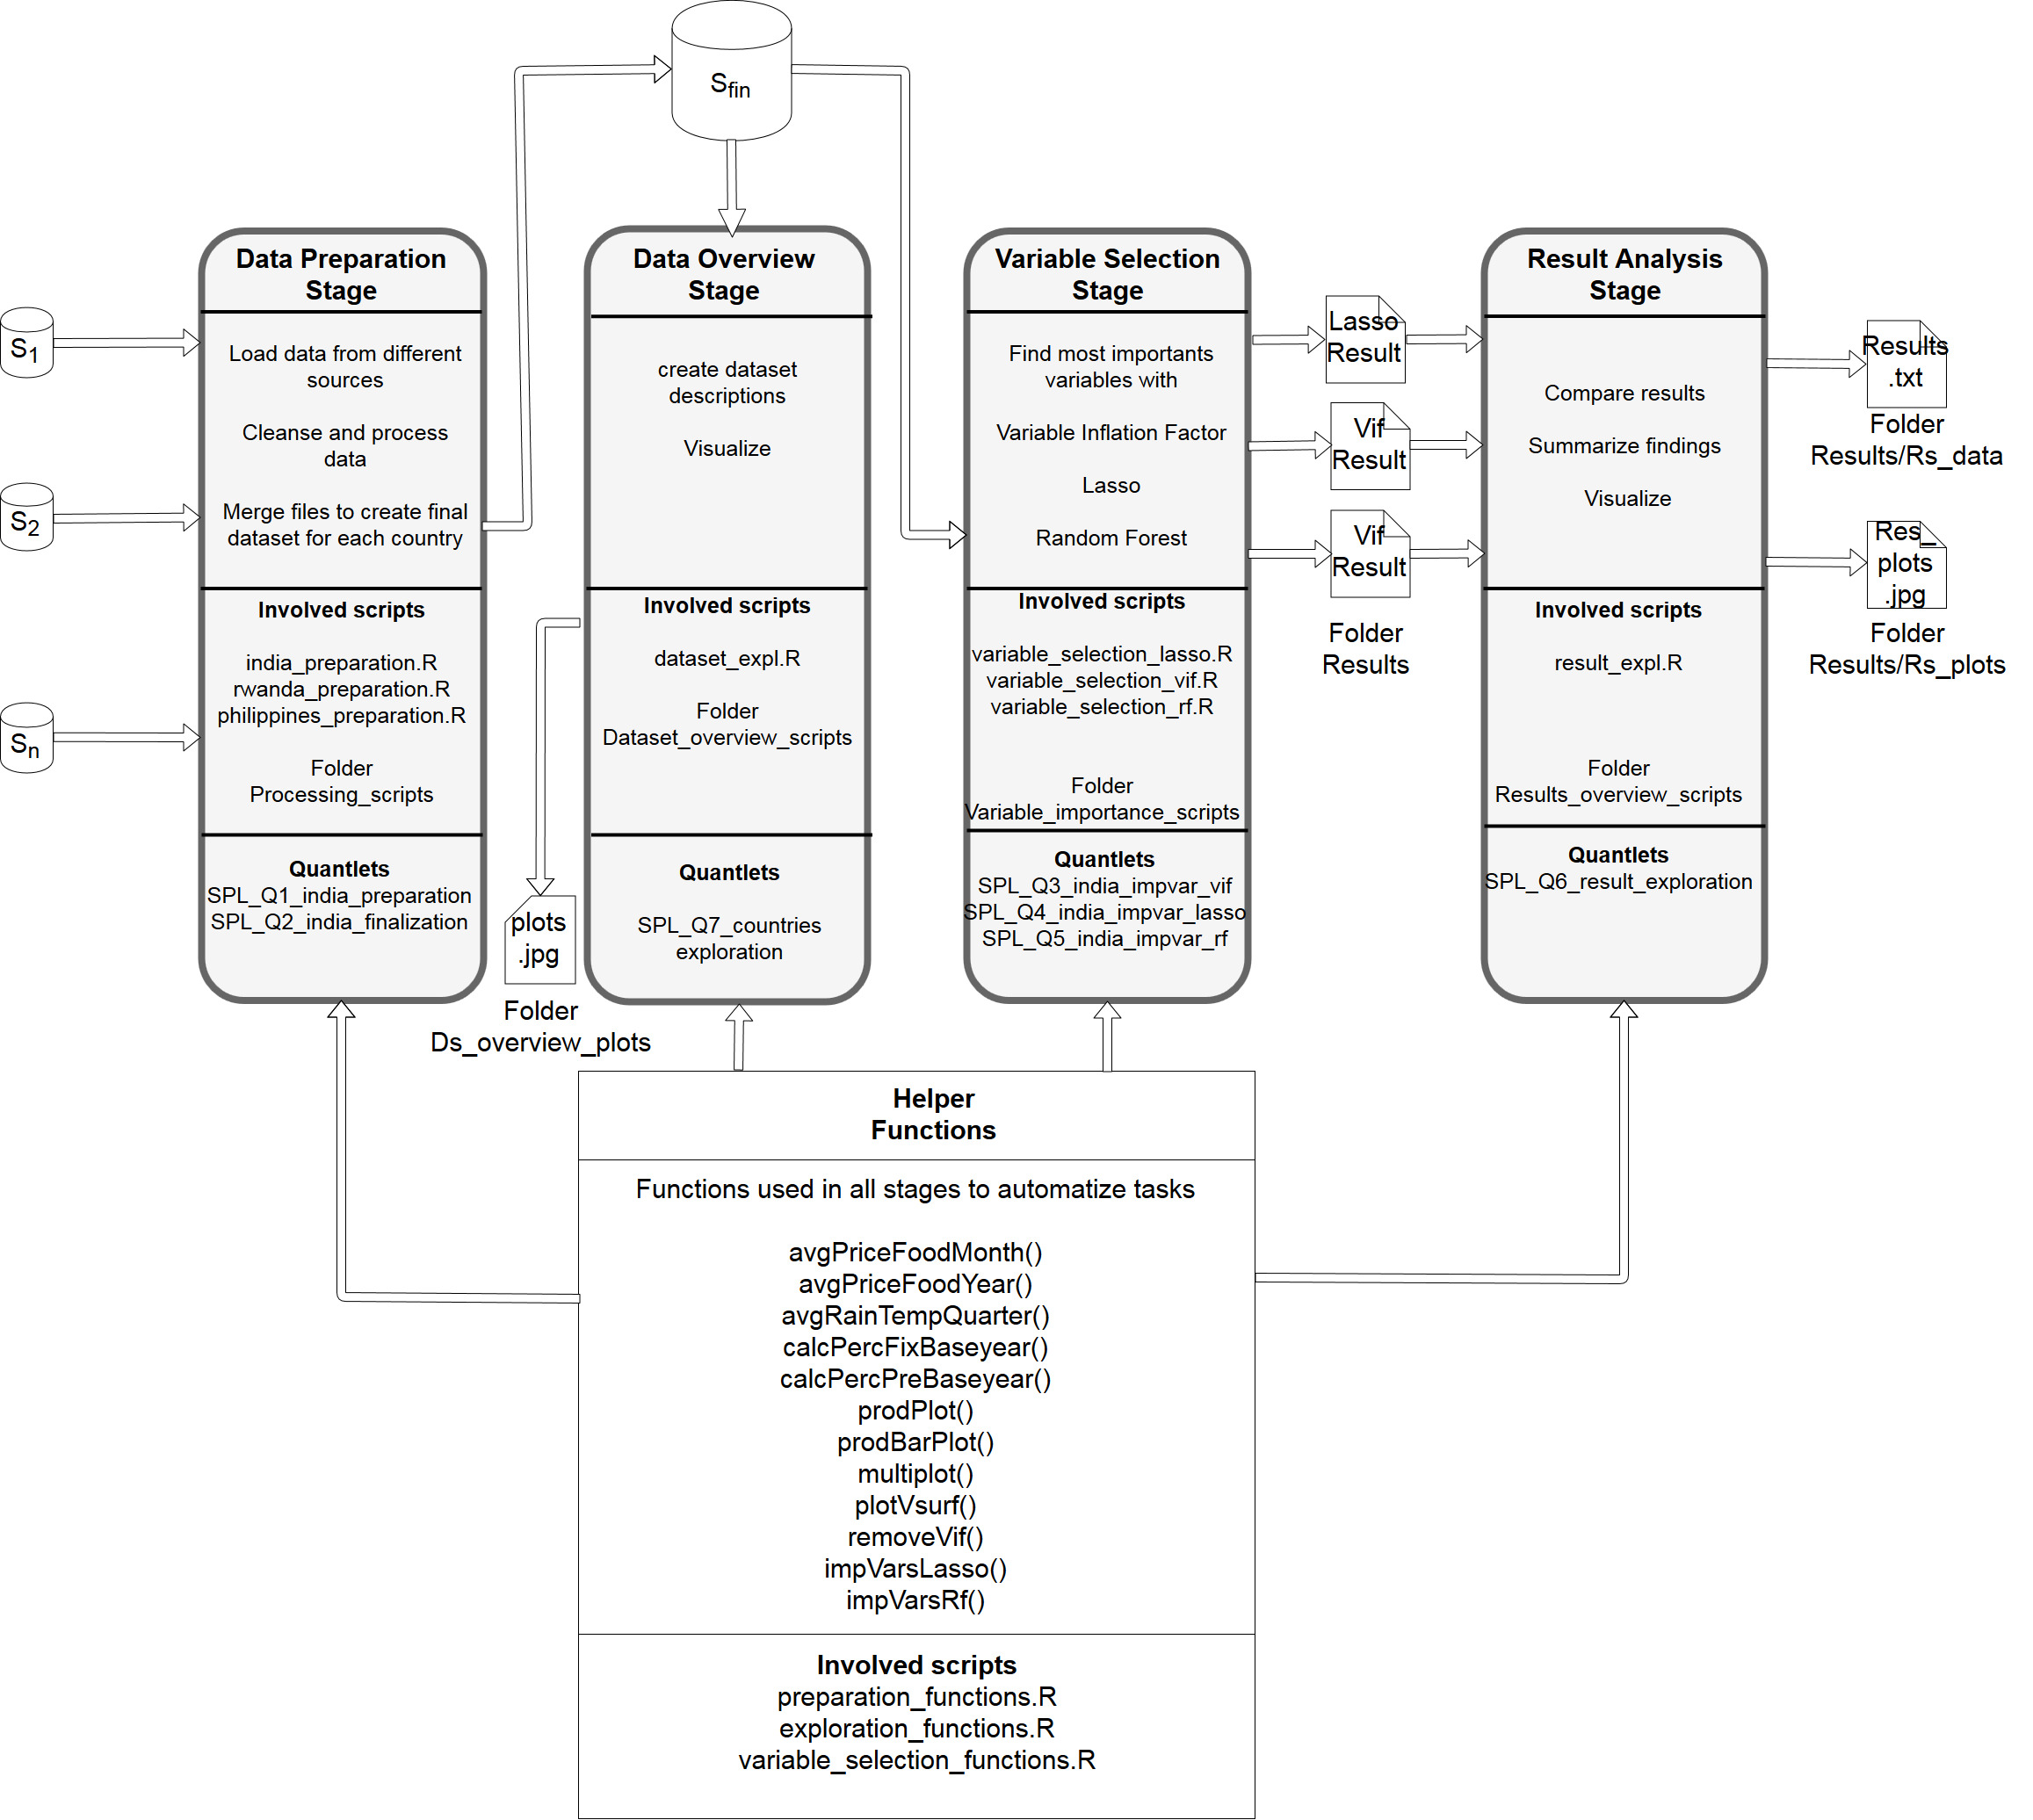
\includegraphics[scale=0.3]{figure1.png}
\caption{Workflow Structure.}
\label{figure1}
\end{center}
\end{figure}
\FloatBarrier

\newpage
In order to build a clean and valid dataset suitable for further analysis, first of all various different pieces of information needed to be taken from a range of different sources and blended together. This is done in the data preparation stage. There is a preparation script for each country we analyzed in the folder Processing\_scripts in our github repository (\url{https://github.com/jaidikam/sps_ws1718}). The scripts make use of utility functions avgPriceFoodMonth(), avgPriceFoodYear() and avgRainTempQuarter() defined in the script preparation\_functions in folder Helper\_functions. Quantlets,SPL\_Q1\_india\_preparation and SPL\_Q2\_india\_finalization serve as a runnable more compact example of all the steps executed in this stage for the country india, independent from our working scripts.
The subsequent data overview stage includes all the steps taken in the explorative analyzation of the datasets created in the previous stage. The script dataset\_expl.R in the folder Dataset\_overview\_scripts holds all the code required to generate graphs such as the development of prices over the years and production rates. The results are stored in .jpeg file format in folder Dataset\_overview\_scripts/Plots. Utility functions used are calcPercFixBaseyear(), calcPercPreBaseyear(), prodPlot() and multiplot() in the script exploration\_functions in folder Helper\_functions. The Quantlet SPL\_Q7 countries\_exploration shows an example of how the explorative graphs were created. 
The next step is to find out the set of important variables for each dataset. This is achieved in the variable selection stage. For each technique, there is a script in the folder Variable\_importance\_scripts. Scripts make use of the functions removeVif(), impVarsLasso(), impVarsRf() defined in the script variable\_selection\_functions.R in the folder Helper\_functions. The resulting Files including the important variables and additional information are stored in folder Results.
The Quantlets SPL\_Q3\_india\_impvar\_vif, SPL\_Q4\_india\_impvar\_lasso, SPL\_Q5\_india\_impvar\_rf show a functionally independent example of how each technique was used in our process.
The final result analysis stage contains all the steps related to display and analyzation of the result files produced in the previous step. Code is included in the working script result\_expl.R in folder Results\_overview\_scripts. For demonstrating purposes there is an independent Quantlet SPL\_Q6\_result\_exploration.









\subsection{Dataset Descriptions}

Dataset description: 
The following tables will showcase the variables used in our datasets. We have three country specific datasets (India, Rwanda and the Philippines) containing information on supply and demand related factors influencing food prices. For the sake of clarity we have split the variables in tables below showing which data is shared by the individual sets and which data is country specific. Information on the variable names, type, range, factor group as well as a description is included. 


The initial table show cases information of the data shared by all three countries: India / Philippines / Rwanda.
\FloatBarrier
\begin{table}[!htbp]
\centering
\begin{adjustbox}{max width=\textwidth}

\begin{tabular}{lllllll}
\hline
VariableName           & DataType & Range(India)        & Range(Philippines)  & Range(Rwanda)       & FactorGroup          & Description                                              \\ \hline
Year                   & int      & 2001-2015           & 1998-2015           & 1991-2015           & x                    & Starting and end year of data collection                 \\
prod\_name             & char     & x                   & x                   & x                   & x                    & name of the selected product                             \\
prod\_price            & num      & 8.392 - 37.02       & 24.70-452.10        & 37.9-1095.9         & supply/production    & ?                                                        \\
tas\_q1                & num      & 19.86-21.64         & 22.826-52.1206      & 18.54-21.13         & supply/climatic      & average temperature in celsius for quartile 1            \\
tas\_q2                & num      & 28.59-30.25         & 11.5366-21.1364     & 19.03-20.90         & supply/climatic      & average temperature in celsius for quartile 2            \\
tas\_q3                & num      & 26.67-27.36         & 15.3575-24.5690     & 19.00-21.26         & supply/climatic      & average temperature in celsius for quartile 3            \\
tas\_q4                & num      & 21.07-22.34         & 15.9073-48.1226     & 19.17-21.42         & supply/climatic      & average temperature in celsius for quartile 4            \\
pr\_q1                 & num      & 7.039-23.189        & 13.4319-61.9415     & 72.86-198.95        & supply/climatic      & average rain fall in mm for quartile 1                   \\
pr\_q2                 & num      & 54.93-109.00        & 16.2071-62.5248     & 45.45-126.96        & supply/climatic      & average rain fall in mm for quartile 2                   \\
pr\_q3                 & num      & 161.3-246.1         & 19.1587-37.5307     & 19.39-135.49        & supply/climatic      & average rain fall in mm for quartile 3                   \\
pr\_q4                 & num      & 21.64-49.27         & 77.865-49.4250      & 85.2-186.9          & supply/climatic      & average rain fall in mm for quartile 4                   \\
avg\_p\_barrel         & num      & 23.12-109.45        & 12.28-109.45        & 12.28-109.45        & supply/production    & annual oil price (U.S. dollars per barrel)               \\
population             & num      & 1.071e+09-1.309e+09 & 74694-101716        & 5928-11630          & demand/demographic   & annual population level                                  \\
prod\_amount           & int      & 41555-362333        & 4106698-28376518    & 2300-3547200        & supply/production    & produced amount in (1k tons)                             \\
gni\_pc                & num      & 778.4-1737.8        & 1784-3163           & 203.8-696.8         & demand/demographic   & per capita income( GNI per capita in constant 2010 US\$) \\
cp\_inflation          & num      & 3.685-11.992        & 1.434-9.235         & -2.406-56.000       & supply/macroeconomic & inflation consumer prices (annual \%)                    \\
agri\_gdp              & num      & 2.092e+11-3.281e+11 & 1.636e+10-2.670e+10 & 4.256e+08-2.098e+09 & supply/macroeconomic & GDP in agriculture value added (constant 2010 US\$)      \\
daily\_caloric\_supply & num      & 2256-2459           & 2292-2595           & 1723-2270           & demand/demographic   & per capita calorie intake (kcal)                         \\
imp\_cer               & int      & 25911-992977        & 27159-117853        & 7625-142335         & supply/macroeconomic & annual imports in thousands of dollars                   \\  \hline

\end{tabular}

\end{adjustbox}
\caption{Data Shared By All Countries}
\label{table1}
\end{table}
\FloatBarrier
\newpage
The following table will showcase information of the data shared by India and Rwanda
\FloatBarrier
\begin{table}[!htbp]
\centering
\begin{adjustbox}{max width=\textwidth}
\begin{tabular}{llllll}
\hline
VarialeName & DataType & Range(India)        & Range(Rwanda) & FactorGroup          & Description                                      \\ \hline
imp\_veg    & num      & 1140825-6317271     & 1954-23112    & supply/macroeconomic & annual vegetable imports in thousands of dollars \\
exp\_cer    & num      & 3.210e+07-2.248e+09 & 0.51-54746.39 & demand/macroeconomic & annual cereal exports in thousands of dollars    \\
exp\_veg    & num      & 851222-3559119      & 43.56-8891.15 & demand/macroeconomic & exported vegetables in US\$    \\        \hline         
\end{tabular}
\end{adjustbox}
\caption{Data Shared By India and Rwanda}
\label{table2}
\end{table}
\FloatBarrier

The next table will showcase information of the data shared by the Philippines and Rwanda.

\FloatBarrier
\begin{table}[!htbp]
\large
\centering
\begin{adjustbox}{max width=\textwidth}
\begin{tabular}{llllll}
\hline
VariableName     & DataType & Range(Rwanda)       & Range(Philippines)  & FactorGroup          & Description                             \\ \hline
GDP              & num      & 7.536e+08-8.261e+09 & 7.221e+10-2.928e+11 & supply/macroeconomic &                                         \\
exchange\_rate   & num      & 125.2-721.0         & 39.09-56.04         & supply/macroeconomic & exchange rate in relation to 2010 US\$  \\
population\_unit & num      & 1000                & 1000                & demand/demographic   & Unit for population size (1000 Persons) \\
flag             & chr      & x                   & x                   & x                    & Country name                            \\
flag.description & chr      & x                   & x                   & x                    & Description of source for country name \\ \hline
\end{tabular}
\end{adjustbox}
\caption{Data Shared by Philippines and Rwanda }
\label{table3l}
\end{table}
\FloatBarrier

The following table will showcase information of the data specific to India
\FloatBarrier
\begin{table}[!htbp]
\small
\centering
\begin{adjustbox}{max width=\textwidth}
\begin{tabular}{lllll}
\hline
VariableName & DataType & Range(India)  & FactorGroup          & Description                            \\  \hline
country      & Factor   & x             & x                    & Country Name                           \\
imp\_sug     & num      & 26034-1419642 & supply/macroeconomic & annual imports in thousands of dollars \\
exp\_sug     & num      & 91273-2247911 & demand/macroeconomic & annual exports in thousands of dollars \\ \hline
\end{tabular}
\end{adjustbox}
\caption{Data Specific to India}
\label{table4l}
\end{table}
\FloatBarrier

The final table will showcase information specific to the Philippines 
\FloatBarrier
\begin{table}[!htbp]
\centering
\resizebox{\columnwidth}{!}{
\begin{tabular}{lllll}
\hline
VariableName & DataType & Range(Philippines) & FactorGroup          & Description \\ \hline
exp\_agri    & num      & 36.30-142.32       & demand/macroeconomic &            \\ \hline
\end{tabular}
}
\caption{Data Specific to Philippines}
\label{table5}
\end{table}
\FloatBarrier

\subsection{Function Descriptions}
\begin{itemize}
\item avgPriceFoodMonth
	\begin{itemize}
	\item description: 
		\begin{itemize}
		\item calculates the average price per month for each product for a given dataframe. 
		\item Adds column avg\_price\_prod\_month.
		\end{itemize}
	\item input parameters: 
		\begin{itemize}
		\item ds: food price data as a dataframe 
		\item cm\_name: the name of the column holding the product name as a String        
		\item mp\_price : the name of the column holding the product price as a String        
		\item mp\_year: the name of the column holding the year as a String       
		\item mp\_month: the name of the column holding the month as a String
		\end{itemize}
	\item output parameters
		\begin{itemize}
		\item ds: the input dataframe including an additional column avg\_price\_prod\_month
		\end{itemize}
	\item typical issues:
		\begin{itemize}
		\item Wrong column name specified: Error  
		\item Column name not passed as String: Error
		\end{itemize}
	\end{itemize}


\item avgPriceFoodYear
	\begin{itemize}
	\item description: 
		\begin{itemize}
		\item calculates the average price per year for each product for a given dataframe 
		\item Adds column avg\_price\_prod\_year.
		\end{itemize}
	\item input parameters: 
		\begin{itemize}
		\item Ds: food price data as a dataframe 
		\item cm\_name: the name of the column holding the product name as a String        
		\item mp\_year: the name of the column holding the year as a String      
		\item avg\_price\_prod\_month: the name of the column holding the average food price per month as a String 
		\end{itemize}
	\item output parameters
		\begin{itemize}
		\item ds: the input dataframe including an additional column avg\_price\_prod\_year
		\end{itemize}
	\item typical issues:
		\begin{itemize}
		\item Wrong column name specified: Error
		\item Column name not passed as String: Error
		\end{itemize}
	\end{itemize}

\item avgRainTempQuarter
	\begin{itemize}
	\item description: 
		\begin{itemize}
		\item Calculates the average temperature and average amount of rain per quarter year for a given dataframe
		\end{itemize}
	\item input parameters: 
		\begin{itemize}
		\item ds: rain and temperature data for every month in each year as a dataframe
		\item month: the name of the column holding the month as a String       
		\item mp\_year: the name of the column holding the year as a String 
		\item pr: the name of the column holding the amount of rain per month as a string
		\item tas: the name of the column holding the average temperature per month as a string
		\end{itemize}
	\item output parameters
		\begin{itemize}
		\item ds: the input dataframe including an additional
		\item columns: tas\_q1, tas\_q2, tas\_q3, tas\_q4, pr\_q1, pr\_q2, pr\_q3, pr\_q4
		\end{itemize}
	\item typical issues:
		\begin{itemize}
		\item Wrong column name specified: Error 
		\item Column name not passed as String: Error
		\end{itemize}
	\end{itemize}

\item plotVsurf
	\begin{itemize}
	\item description: 
		\begin{itemize}
		\item Plots VSURF objects for thresholding and interpretation step
		\end{itemize}
	\item input parameters: 
		\begin{itemize}
		\item iVsurfOb: A VSURF object
		\item iStep: the step for which results are to be plotted as a string 
		\item iCountry: the country for which results are to be plotted as a string  
		\end{itemize}
	\item typical issues:
		\begin{itemize}
		\item Other object than VSRUF object passed to function
		\item Other string than "thres" or "interp" passed as value for iStep
		\end{itemize}
	\end{itemize}

\item removeVif
	\begin{itemize}
	\item description: 
		\begin{itemize}
		\item Removes multicorrelated numeric variables from a given dataframe based on variance inflation factor
		\end{itemize}
	\item input parameters: 
		\begin{itemize}
		\item explan\_vars: the numeric variables as a dataframe
		\item cutoffval: the maximum allowed vif for remaining variables as a number
		\end{itemize}
	\item output parameters
		\begin{itemize}
		\item tempresults: the remaining variable names and their corresponding vif as a dataframe
		\end{itemize}
	\item typical issues:
		\begin{itemize}
		\item non numeric variables in input dataframe
		\end{itemize}
	\end{itemize}

\item impVarsLasso
	\begin{itemize}
	\item description: 
		\begin{itemize}
		\item Identifies important variables for a given dataframe based on the lasso method
		\end{itemize}
	\item input parameters: 
		\begin{itemize}
		\item ds: the variables as a dataframe
		\item targ: the name of the target variable column in ds as a String
		\end{itemize}
	\item output parameters
		\begin{itemize}
		\item resultset: the lasso model, fitted model and the label for display in a graph as a vectorlist   
		\end{itemize}
	\item typical issues:
		\begin{itemize}
		\item Column name not passed as String: Error
		\end{itemize}
	\end{itemize}

\item impVarsRf
	\begin{itemize}
	\item description: 
		\begin{itemize}
		\item Identifies important variables for a given dataframe based on MSE error minimization in OOB samples of random forest
		\end{itemize}
	\item input parameters: 
		\begin{itemize}
		\item ds: the variables as a dataframe
		\item targ: the name of the target variable column in ds as a String
		\end{itemize}
	\item output parameters
		\begin{itemize}
		\item resultset: names of important variables and mean OOB rate as a vectorlist
		\end{itemize}
	\item typical issues:
		\begin{itemize}
		\item Column name not passed as String: Error
		\end{itemize}
	\end{itemize}

\item calcPercFixBaseyear 
	\begin{itemize}
	\item description: 
		\begin{itemize}
		\item calculate the percentage of the change in a column's value based on a fixed year
		\end{itemize}
	\item input parameters: 
		\begin{itemize}
		\item ds: the variables as a dataframe
		\item areacol: name of the column holding the areas  as a String
		\item areaname: name of selected area
  		\item yearcol: name of the column holding the years as a String
		\item baseyear: selected bese year 
		\item valuecol:  name of the target column holding the values as numbers for the calculation
		\item perccol:  name of the new generated column holding the results of the calculations
		\end{itemize}
	\item output parameters
		\begin{itemize}
		\item ds: the input dataframe including an newly generated column 
		\end{itemize}
	\item typical issues:
		\begin{itemize}
		\item the newly generated column is not identified at the first assignment: Error
		\end{itemize}
	\end{itemize}

\item calcPercPreBaseyear  
	\begin{itemize}
	\item description: 
		\begin{itemize}
		\item calculate the percentage of changes in a column's values in a predefined year, where the base is for every change is the value from the previous year.
		\end{itemize}
	\item input parameters: 
		\begin{itemize}
		\item ds: the variables as a dataframe
		\item areacol: name of the column holding the areas  as a String
		\item areaname: name of selected area
  		\item yearcol: name of the column holding the years as a String 
		\item valuecol:  name of the target column holding the values as numbers for the calculation
		\end{itemize}
	\item output parameters
		\begin{itemize}
		\item ds: the input dataframe including an newly generated column 
		\end{itemize}
	\item typical issues:
		\begin{itemize}
		\item At the loop the previous has a value but the later year not: Divide by Zero Error
		\end{itemize}
	\end{itemize}

\item prodPlot   
	\begin{itemize}
	\item description: 
		\begin{itemize}
		\item plot production data with specific area and items
		\end{itemize}
	\item input parameters: 
		\begin{itemize}
		\item ds: the variables as a dataframe
		\item area: name of the selected area as a String
		\item items: name of the selected Items as a sequence of Strings
		\end{itemize}
	\item output parameters
		\begin{itemize}
		\item p: a plot showing the percentage change in production quantities, based on a specific area and items
		\end{itemize}
	\end{itemize}

\item prodBarPlot   
	\begin{itemize}
	\item description: 
		\begin{itemize}
		\item plot production data with specific area and items
		\end{itemize}
	\item input parameters: 
		\begin{itemize}
		\item ds: the variables as a dataframe
		\item dnmae: name of the selected area as a String
		\end{itemize}
	\item output parameters
		\begin{itemize}
		\item p: a plot showing the percentage change in product's price, based on a specific area 
		\end{itemize}
	\end{itemize}



\end{itemize}


\newpage
\section{Implementation}

This section gives detailed information about the actual implementation of every step featured in \textbf{Section 2} including r code and theoretical background of every variable technique that was applied.



\subsection{Data Preparation}

In order to get comparable results, it was necessary to work with datasets containing comparable features. After specifying which variables were supposed to be included in the final datasets, those information needed to be put together from a range of heterogenous sources. 
The source dataset containing food prices, for an instance, included the monthly price of each crop of interest for each marketplace in a certain country. That made it necessary to calculate the average price per crop per month for the whole country which is done by the following function:


\begin{lstlisting}[language= R, captionpos=b,caption=\href{https://github.com/jaidikam/sps_ws1718/tree/master/Qfolder1}{SPL\_Q1\_india\_preparation}]
#Define the function for food price per month across all markets
avgPriceFoodMonth = function(ds,cm_name,mp_price,mp_year,mp_month){
  dsfoods = unique(ds[[cm_name]])
  ds$avg_price_prod_month = 0
  for (k in min(ds[[mp_year]]):max(ds[[mp_year]])){
    print(paste('year is ',k))
    for (j in 1:NROW(dsfoods)){
      a <- ds[ds[[mp_year]] == k & ds[[cm_name]] == dsfoods[j],]
      print(paste('food is ',dsfoods[j]))
      for (i in 1:12){
        b <- a[a[[mp_month]] == i,]
        if (NROW(ds[ds[[mp_year]] == k & ds[[cm_name]] == dsfoods[j] & ds[[mp_month]] == i,]$avg_price_prod_month) >0) {
          ds[ds[[mp_year]] == k & ds[[cm_name]] == dsfoods[j] & ds[[mp_month]] == i,]$avg_price_prod_month =  sum(b[[mp_price]])/ NROW(b)
          print(paste('month is ',i))  
        } 
      }
    }
  }
  return(ds)
}
india = avgPriceFoodMonth(india,"cm_name","price","year","month")
\end{lstlisting}

Function avgPriceFoodMonth takes the dataframe containing price information and allows the user to explicitly pass the names of the columns holding relevant information as strings.
First, possible duplicates in the input dataset are removed and the name of every crop is stored in a variable dsfoods. Then a column avg\_price\_prod\_month to hold the result is added to the dataset with value 0 .
The first most outer loop iterates through the year. The second loop goes through every crop. The most inner loop goes through every month for every possible year/crop pair. If rows exist for a certain month/year/crop combination, the sum of prices for that combination are devided by the number of occurrences resulting in the desired average. The if – condition is necessary to avoid the possibility to divide by 0. Finally, the dataframe plus the newly created column is returned.

Later on in the process we decided to look at crop prices per year, so we created another similar function to calculate the average price per food per year:

\begin{lstlisting}[language= R, captionpos=b,caption=\href{https://github.com/jaidikam/sps_ws1718/tree/master/Qfolder2}{SPL\_Q2\_india\_preparation}]
avgPriceFoodYear = function(ds,cm_name,mp_year,avg_price_prod_month){
  dsfoods = unique(ds[[cm_name]]) 
  ds$avg_price_prod_year = 0
  for (x in min(ds[[mp_year]]):max(ds[[mp_year]])){
    print(paste('year is ',x))
    for(y in 1:NROW(dsfoods)){
      print(paste('food is ',dsfoods[y]))
      if(NROW(ds[ds[[mp_year]] == x & ds[[cm_name]] == dsfoods[y],]$avg_price_prod_year) > 0){
        ds[ds[[mp_year]] == x & ds[[cm_name]] == dsfoods[y],]$avg_price_prod_year = sum(ds[ds[[mp_year]] == x & ds[[cm_name]] == dsfoods[y],][[avg_price_prod_month]]) / NROW(ds[ds[[mp_year]] == x & ds[[cm_name]] == dsfoods[y],][[avg_price_prod_month]])
      }
    }
  }
  return(ds)
}
india  = avgPriceFoodYear(india,"cm_name","year","avg_price_prod_month")
\end{lstlisting}

The function takes a dataframe including crop prices on a monthly level and allows the user to specify the columns holding crop name, year and price per month.
We pass the dataset that was created by the previous function and the column for the average price per year is added. The outer loop iterates through the years, the inner loop goes through the list of unique crop names. For every existing year/crop combination the average is price calculated.

Another dataset that required processing was the climate set, containing the amount of rain and the temperature for every month in a year, each in a column of its own. Instead of one row per month, we needed the average amount of rain / temperature for each quarter of the year to be a row identified by the year.
A function was written to achieve that:

\begin{lstlisting}[language= R, captionpos=b,caption=\href{https://github.com/jaidikam/sps_ws1718/tree/master/Qfolder2}{SPL\_Q2\_india\_finalization}]
avgRainTempQuarter = function(ds,month,mp_year,pr,tas){
  if (is.na(ds[[pr]]) ||is.na(ds[[tas]])) {
    message(paste("No missing values allowed!"))
  } else {
    ds$tas_q1 = 0
    ds$tas_q2 = 0
    ds$tas_q3 = 0
    ds$tas_q4 = 0
    ds$pr_q1  = 0
    ds$pr_q2  = 0
    ds$pr_q3  = 0
    ds$pr_q4  = 0
    
    for(z in min(ds[[mp_year]]):max(ds[[mp_year]])){
      
      ds[ds[[mp_year]] == z ,]$pr_q1  =   sum(ds[ds[[mp_year]] == z & ds[[month]] %in% c("1","2","3"),][[pr]])/3
      ds[ds[[mp_year]] == z ,]$pr_q2  =   sum(ds[ds[[mp_year]] == z & ds[[month]] %in% c("4","5","6"),][[pr]])/3
      ds[ds[[mp_year]] == z ,]$pr_q3  =   sum(ds[ds[[mp_year]] == z & ds[[month]] %in% c("7","8","9"),][[pr]])/3
      ds[ds[[mp_year]] == z ,]$pr_q4  =   sum(ds[ds[[mp_year]] == z & ds[[month]] %in% c("10","11","12"),][[pr]])/3
      ds[ds[[mp_year]] == z ,]$tas_q1 =   sum(ds[ds[[mp_year]] == z & ds[[month]] %in% c("1","2","3"),][[tas]])/3
      ds[ds[[mp_year]] == z ,]$tas_q2 =   sum(ds[ds[[mp_year]] == z & ds[[month]] %in% c("4","5","6"),][[tas]])/3
      ds[ds[[mp_year]] == z ,]$tas_q3 =   sum(ds[ds[[mp_year]] == z & ds[[month]] %in% c("7","8","9"),][[tas]])/3
      ds[ds[[mp_year]] == z ,]$tas_q4 =   sum(ds[ds[[mp_year]] == z & ds[[month]] %in% c("10","11","12"),][[tas]])/3
    }
    return(ds)
  }  
}
raintemp  = avgRainTempQuarter(raintemp,"month","year","pr","tas") 
#load the india dataset and the remaining variables
india_wip = readRDS(".\\Qfolder1\\Q1_india_wip.rds")
rest      = readRDS(".\\Qfolder2\\Q2_india_rest.rds")
#merge india with wheater data
india_wip = merge(india_wip,unique(raintemp[c("tas_q1","tas_q2","tas_q3","tas_q4","pr_q1","pr_q2","pr_q3","pr_q4","year")]),by=c("year")) 
#join the datasets
india_fin = merge(india_wip, rest, by=c("prod_price"))  #prod_price is unique, therefore it can be used as a key for the merge
\end{lstlisting}

The function takes a the climate dataset and allows the user to pass strings to identify the columns holding the month, year, rain and temperature respectively. Given that the dataset has no missing values in the rain and the temperature column, additional columns are added for every quarter of the year and the filled with the sum of each quarter divided by the number of month a quarter year has.
The dataset with the added columns is then returned. Afterwards, the datasets are merged to create the final dataset used in the next step.

\subsection{Data overview}

In this section we will explain the process and the code which we used to produce four of our graphs, which provide us with some important statistical comparison. All the produced graphs are mmentioned in \textbf{Section 4.1}
The resulted graphs were: 
\begin{itemize}
\item Product Price Change 
\item Population Change 
\item Price Index 
\item Consumer Price Development 
\end{itemize}

We have collected our databases from different resources, and for the values to be comparable between countries an world wide, we had to develop some functions to calculate the percentage of the change
\begin{lstlisting}[language= R, captionpos=b,caption=\href{https://github.com/jaidikam/sps_ws1718/tree/master/Qfolder7}{SPL\_Q7\_countries\_exploration.R}]
#calculating the percentage of the change in a column's value on a fixed base year 
calcPercFixBaseyear =  function(ds, areacol, areaname, yearcol, baseyear,valuecol, perccol){
  base = ds[ds[[yearcol]] == baseyear & ds[[areacol]] %in% areaname, ][[valuecol]]
  if(is.null(ds[[perccol]])){
    ds[[perccol]] = 0 
  }
  #
  for(i in baseyear: max(ds[[yearcol]])){
    later = ds[ds[[yearcol]]==i & ds[[areacol]] %in% areaname,][[valuecol]]
    sub =  later - base
    ds[ds[[yearcol]] == i & ds[[areacol]] %in% areaname,][[perccol]] = (sub / later) * 100
  }
  return(ds)
}
\end{lstlisting}
Function calcPercFixBaseyear calculates the precentage change in a value basd on a specifed base year during a timeframe, where the percentage will always represent the difference between the cvalue column and the value stored in the base year, beside the base year the function takes also targeted dataframe,  area column, area name, year column, value column and the name of the produced new column. 
We firstly store the given year in the base variable then we check if the goal new column have been already identified or not. After that we go through a loop in value column depending on the targeted year column and store the resulted percentage change in the new column and at the the end returning the new dataframe comntain the newly calculated column for the specified area during the the specifed time duration. 

\begin{lstlisting}[language= R, captionpos=b,caption=\href{https://github.com/jaidikam/sps_ws1718/tree/master/Qfolder7}{SPL\_Q7\_countries\_exploration.R}]
# calculate the percentage of changes in a colname value in a predefined year, where the base is for every change is the value from the previous year.
calcPercPreBaseyear = function(ds, areacol, areaname, yearcol, valuecol){
  for(i in unique(ds[[yearcol]])){
    base = ds[ds[[yearcol]] == i & ds[[areacol]] %in% areaname, ][[valuecol]]
    later = ds[ds[[yearcol]] == i+1 & ds[[areacol]] %in% areaname, ][[valuecol]]
    #if(length(later) == 0L) break
    if(i == 2015L) break
    sub =  later - base
    if(length(sub) == 0L)next 
    ds[ds[[yearcol]] == i+1 & ds[[areacol]] %in% areaname , paste(valuecol, "Percent", sep = "_")]= (sub / later) * 100
  }
  ds[ds[[yearcol]] == min(ds[[yearcol]]) & ds[[areacol]] %in% areaname, paste(valuecol, "Percent", sep = "_")]= 0
  return(ds)
}
\end{lstlisting}

Function calcPercFixBaseyear also calculate the precentage change, but this time the base year is changing and is not fixed, it takes the value of the pervious year at each calculation for a value in a specific year   

\begin{lstlisting}[language= R, captionpos=b,caption=\href{https://github.com/jaidikam/sps_ws1718/tree/master/Qfolder7}{SPL\_Q7\_countries\_exploration.R}]
# To plot production data with specific area and itmes
prodPlot = function(ds, area, items){
  p = ggplot(data=ds[ds$Area == area & ds$Item %in% items,], aes(x=Year, y=Percentage, colour=Item)) +
    geom_line() +
    geom_point()+
    ylim(-30, 75)+
    ggtitle(label=area)+
    ylab(label="Percentage Production Change") +
    xlab("Year")
  return(p)
}
\end{lstlisting}
We use prodPlot function to produce the six graphs in \textbf{Figure 5. Consumer Price development}, where it show us the change of the products prices in the studied countries in compare the world wide change. The function takes the dataframe along side the area name and targeted items, then it produce the plot for the defined parameters. 


\subsection{Variable Selection}

To find out which variables have the biggest impact on food prices, we apply three techniques which were implemented as follows:

\subsubsection{VIF based method}

Before fitting a linear model, first of all it is necessary to check for correlation among explanatory variables, since high correlation means that variables are not independent from one another As a way to measure the degree of dependence of variable pairs, Pearson’s correlation coefficient was used.
Intuitively, explanatory variables should only be correlated to the target variable, not to each other. Otherwise the model will have high standard deviation and therefore high variance and possibly low predictive power. Also significant variables may appear non-significant.
However, pair-wise analysis for correlation may not reveal multicollinearity, i.e. a situation where a predictor can be explained through the other predictors. Multicollinearity is excessive correlation among several explanatory variables. A commonly used way to detect that is a metric called variance inflation factor. It helps to quantify the amount of variance that each predictor adds to the model.
To calculate the VIF for a variable $b_{k}$,
Given a linear model :  
 \begin{center} \[ \scalebox{1.5} {$y_{i} = \beta_{0}+\beta_{1}x_{i1}+$...$+\beta_{k}x_{ik}+$...$+\beta_{p-1}x_{i,p-1}+\epsilon_{i} $ }\] \end{center}

By regressing $b_{k}$ with only one of the other predictors at a time we calculate the variances for $ b_{k}$.
We keep the smallest variance, obtained by: 
\begin{center} \[ \scalebox{1.5} {$Var(b_{k})_{min} = \frac{\delta^2 }{\sum_{i=1}^{n}(x_{ik} - \overline{x}_{k})^2}$}\]  \end{center}

In order to find out how much $b_{k}$ increases the overall variance of the model we get the ratio of $Var(b_{k})_{min}$ and $Var(b_{k})$, the variance of $b_{k}$ when all remaining variables are regressed on $b_{k}$ at the same time:

\begin{center}  \[ \scalebox{1.5} {$\frac{Var(b_{k})}{Var(b_{k})_{min}}=\frac{\left ( \frac{\delta^2 }{\sum_{i=1}^{n}(x_{ik} - \overline{x}_{k})^2} \times \frac{1}{1-R^2_{k}} \right )}{(\frac{\delta^2 }{\sum_{i=1}^{n}(x_{ik} - \overline{x}_{k})^2})}=\frac{1}{1-R^2_{k}}$}\] \end{center}

$R^2_{k}$ is the $R^2$ value when the $ k^{th}$ is regressed on all remaining explanatory variables

It follows : 
\begin{center}  \[ \scalebox{1.5} {$VIF_k  =\frac{1}{1-R^2_{k}}$}\] \end{center}

The correlation- and VIF based method was implemented as follows:
After choosing the explanatory variables and standardizing them we acquire the correlation coefficient for each pair:

\begin{lstlisting}[language= R, captionpos=b,caption=\href{https://github.com/jaidikam/sps_ws1718/tree/master/Qfolder3}{SPL\_Q3\_india\_impvar\_vif}]
#initial variable selection and normalization
colselection_in = c("prod_price","pr_q1","pr_q2","pr_q3","pr_q4","tas_q1","tas_q2","tas_q3","tas_q4",
                    "prod_amount","daily_caloric_supply","exp_sug","exp_veg","exp_cer","imp_sug","imp_veg","imp_cer", 
                    "agri_gdp","gni_pc","cp_inflation","avg_p_barrel","population") 
target_in = c("prod_price")
normalized_in = as.data.frame(scale(india[colselection_in]))
feats_in = normalized_in[, !(colnames(normalized_in) %in% target_in)]
#Variable selection and modeling
#Obtaining pair-wise correlations 
insign_in = cor( feats_in, method = "pearson", use = "complete.obs")
\end{lstlisting}

After we calculated the correlations for each pair, every variable being part of a pair with a correlation coefficient above 0.70 is removed and a linear model is built.
\begin{lstlisting}[language= R, captionpos=b,caption=\href{https://github.com/jaidikam/sps_ws1718/tree/master/Qfolder3}{SPL\_Q3\_india\_impvar\_vif}]
# Discovering highly correlated explanatory variables
hicorvars_in = findCorrelation(cor(feats_in), cutoff = 0.70)
expvarsnohc_in = paste(colnames(feats_in[,-hicorvars_in]), collapse = "+")
formulanohc_in = paste(target_in,"~",expvarsnohc_in,collapse = "+")
mod_varnohc_in = lm(formulanohc_in,data = normalized_in)
#For comparison we also apply the VIF-based method to tackle multicollinearity:
#function for VIF based stepwise removal of multicorrelated variables
removeVif = function(explan_vars,cutoffval=10){
  tempresults = as.data.frame(matrix(ncol = 2, nrow = 0))
  colnames(tempresults) = c("variable","vif")
  #initially calculate VIF for each explanatory variable
  for (i in 1:NROW(colnames(explan_vars)) ){
    temptarget = colnames(explan_vars)[i]
    tempexpvars = paste(colnames(explan_vars[,!(colnames(explan_vars) %in% temptarget)]),collapse = "+")
    tempformula = paste(temptarget,"~", tempexpvars, collapse = " ")
    tempresults[i,1] = temptarget 
    tempresults[i,2] = VIF(lm( tempformula,data = explan_vars))
  }
  print(tempresults[order(tempresults$vif),])
  #remove variable with highest VIF, calculate new VIF for remaining variables until all VIF are below cutoff value
  while(max(tempresults$vif) >= cutoffval){
    tempresults = tempresults[!tempresults$vif == max(tempresults$vif),]
    tempremvars = tempresults$variable
    for(j in 1: NROW(tempremvars)){
      temptarget = tempremvars[j]
      tempexpvars = paste(tempremvars[!tempremvars %in% temptarget],collapse = "+")
      tempformula = paste(temptarget,"~", tempexpvars, collapse = " ")
      tempresults[j,1] = temptarget 
      tempresults[j,2] = VIF(lm( tempformula,data = explan_vars))
    }
    print("Remaining variables:")
    print(tempresults[order(tempresults$vif),])
    cat("\n") 
  }
  return(tempresults)
}
# for highly correlated variables
varslovifhc_in = removeVif(feats_in[,hicorvars_in],8) 
# for lower correlated variables
varslovifnohc_in = removeVif(feats_in[,-hicorvars_in],8) 
#Model without multicolinearity
expvars_lovif_in = paste(paste(varslovifhc_in$variable,collapse = "+"),"+",paste(varslovifnohc_in$variable,collapse = "+"),collapse = "+")
formula_lovif_in = paste(target_in,"~",expvars_lovif_in,collapse = "+")
mod_lovif_in = lm(formula_lovif_in,data = normalized_in)
\end{lstlisting}

The function takes a dataframe containing explanatory variables and a cutoff value that specifies the highest admissible VIF until the function stops removing variables. The r package “fmsb” is required.

The first loop iterates through each explanatory variable and regresses them on the remaining variables
to obtain its VIF. Subseqently the while loops conducts the following steps until no more variables with
VIF > threshold value remain:

1.Remove the variable with highest VIF
2.In the inner for loop iteratively calculate VIF for remaining variables

Finally, the function returns a dataframe containing the remaining variables and their VIF values

The function is applied to all the highly pair-wise correlated variables identified  as well as to the remaining less correlated variables in a separate call. The linear model is then constructed from the remaining predictors and saved as a file.

\subsubsection{Lasso based method}

Lasso (Least Absolute Shrinkage and Selection Operator) is a regression based method for regularization and feature selection. A constraint is put on the absolute sum of model parameters and a penalty is applied to the regression coefficients. The strength of the penalty is defined by the parameter lambda. The bigger lambda gets, the sooner model parameters exceed the threshold value and get dropped from the model. Intuitively, a smaller lambda causes more parameters to stay in the model. Lambda = 0 means there is no penalty at all and the regression becomes an ordinary least square regression
Formulation by(Bühlmann \& Van de Geer 2010).

Find a solution to the optimization problem 
minimize 
\begin{center}  \[ \scalebox{1.5} {$\left ( \frac{||Y-X\beta ||^2_2}{n} \right )$ subject to  $\sum_{j=1}^{k} ||\beta ||_1<t$}\] \end{center} 

t is the upper bound for the sum of the coefficients.
Which is equivalent to the parameter estimation \\ 
\begin{center}  \[ \scalebox{1.5} {$\arg \min_{]\beta}\left (\frac{||Y-X\beta||_{2}^2}{n} +\lambda ||\beta ||_{1} \right ) $}\] \end{center} 

Where
\begin{center} \[ \scalebox{1.5} {$\frac{||Y-X\beta||_{2}^2}{n} = \sum _{i=0}^n\left ( Y_{i}-(X\beta)_{i} \right )^2, ||\beta||_{1}=\sum _{j=1}^k|\beta_{j}| and \lambda \geq 0 $}\]\end{center} 

If $\lambda$ gets 0, t becomes infinite and vice versa
In other words, we find the set of coefficients from the model having the least mean squared error for  a sequence of descending lambdas

For application of the lasso method, a function was written:
Our implementation of the lasso technique requires the r packages "glmnet" and "plyr"

\begin{lstlisting}[language= R, captionpos=b,caption=\href{https://github.com/jaidikam/sps_ws1718/tree/master/Qfolder4}{SPL\_Q4\_india\_impvar\_lasso}]
#function for LASSO method   
impVarsLasso = function(ds,targ){
  #1. initial variable selection and normalization
  val = ds[[targ]]
  x = model.matrix(ds[[targ]]~.-1 , ds[!colnames(ds) %in% targ])
  #2. Applying the Lasso technique
  lasso = glmnet(x = x, y = val,  standardize = TRUE, alpha = 1)
  fit   = cv.glmnet(x = x, y = val, standardize = TRUE, type.measure ="mse", alpha=1, nfolds=3) 
  #3. Results
  #with lambda.min
  lambda_min = which(fit$lambda == fit$lambda.min) 
  #selecting coefficients of variables at lambda where mse is minimal
  tempmincoefs             = as.data.frame(fit$glmnet.fit$beta[, which(fit$lambda == fit$lambda.min)])
  mincoefs                 =  data.frame(matrix(ncol = 2, nrow = (NROW(tempmincoefs))))
  mincoefs$variables       = as.vector(as.character(labels(tempmincoefs)[[1]]))
  mincoefs$coefs_minlambda = as.vector(tempmincoefs[[1]])
  mincoefs$X1              = NULL
  mincoefs$X2              = NUL 
  #get names in the decreasing order they appear in when lambda is minimal
  names           = names(coef(lasso)[,ncol(coef(lasso))][order(coef(lasso)[,ncol(coef(lasso))],decreasing=TRUE)])
  names           = names[!names %in% c("(Intercept)")]
  names           = as.data.frame(names)
  colnames(names) = "variables" 
  #add coefficient to names
  disp_colors = join(names,mincoefs, by = "variables" )
  disp_colors = disp_colors[!disp_colors$variables %in% c("(Intercept)"),] 
  #set colors for variables  when displayed in a graph
  disp_colors$colors = 0
  if(NROW(disp_colors[disp_colors$coefs_minlambda >0,])>0){
    disp_colors[disp_colors$coefs_minlambda >0,]$colors = c("green")
  }
  if(NROW(disp_colors[disp_colors$coefs_minlambda <0,])>0){
    disp_colors[disp_colors$coefs_minlambda <0,]$colors = c("red")
  }  
  #create a list to store the result
  resultset =  vector("list",3)
  resultset[[1]] = lasso
  resultset[[2]] = fit
  resultset[[3]] = disp_colors
    return(resultset)
}
#Get most important variables with Lasso function
india_lasso_result = impVarsLasso(india,"prod_price")
\end{lstlisting}

The function takes a dataframe as input and allows the user to specify the column holding the target variable by passing the name as a string.
In line 21 a glmnet model is built, applying the aforementioned lasso method.
Then a fitted model is built in the same way. The mean square error of each model for every lambda is calculated using three-fold cross validation for better generalization of the results, i.e. to avoid overfitting.
In the following step the coefficients and variable names from the model with the lowest MSE are stored in a dataframe called mincoefs. In order to offer additional information about the correct color when the results are plotted, the variables names are ordered in the decreasing order they appear in when lambda is minimal, i.e. when their curves would cut the right margin of the plot. If coefficients in mincoeffs are greater 0, they will be displayed in green in the graph, lower 0 in red, all other will be grey.
Finally, the model, fitted model and the display information are stored in a list which is then returned



\subsubsection{Random Forest based method}

The third variable selection technique we applied is based on random forests.
Random forests are a non-parametrical statistical method used for regression and classification problems. RF are an ensemble of decision trees built from samples of the whole data. The importance of a variable $X^j$ is calculated as follows: Each tree t runs a prediction on the Out of bag sample $OOB_{t}$ (the portion of data not included in the sample to create t). The mean square error MSE of this prediction is denoted $errOOB_{t}$. Now the values for $X^j$ in $OOB_{t}$ are permuted randomly to get a perturbed sample ${OOB}^j_{t}$. Then the error ${errOOB}^j_{t}$ of t on the perturbed sample is calculated. Now the variable importance for $X^j$ is computed as follows:
\begin{center}  \[ \scalebox{1.5} {$VI(X^j)=\frac{1}{ntree}\sum_{t}\left ( \widetilde{errOOB}^j_{t} - errOOB_{t} \right )$}\] \end{center}

The function used to obtain the most important variables using RF requires the r package “VSURF” 
The implementation utilizes a two-step approach to find the most important variables:
\begin{itemize}
\item Threshold step
After computing the VI, each variable is ranked by VI in descending order.
Variables with small importance are eliminated. The threshold is derived from the standard deviations of VI. Important variables have a higher variability so only variables with a averaged VI exceeding the threshold are kept in the model
\item Variable Selection
Interpretation step: 
A nested collection of RF models is built for the first k to m variables. The variables leading to the minimal OOB error are selected, resulting in m’ variables being retained.
Prediction step:
The variables from the interpretation step are ordered and sequentially added to an RF model. Variables which lead to an error decrease above a certain threshold are kept.
\end{itemize}
Note: Since prediction step focuses on predictive power of the model, some variables that in fact have an influence on the target are removed since others are stronger predictors. Our focus lies on generally identifying variables having a significant influence on the target, therefore the prediction step is ignored in our approach.

\begin{lstlisting}[language= R, captionpos=b,caption=\href{https://github.com/jaidikam/sps_ws1718/tree/master/Qfolder5}{SPL\_Q5\_india\_impvar\_rf}]
#function for finding most important variables based on random forest  
impVarsRf = function(ds,targ){
  result_rf = VSURF(ds[[targ]] ~ ., data = ds[!colnames(ds) %in% targ], ntree = 2000,
                    nfor.thres = 50, nmin = 1, nfor.interp = 25, nsd = 1,
                    nfor.pred = 25, nmj = 1, parallel = FALSE, ncores = detectCores() - 1,
                    clusterType = "PSOCK")
  #create a list to store the result
  resultset =  vector("list",2)  
  resultset[[1]] = result_rf
  resultset[[2]] = colnames(ds[!colnames(ds) %in% targ])
  return(resultset)
}
#apply the function
india_v_imp_rf = impVarsRf(india,"prod_price")
\end{lstlisting}

\subsection{Result Exploration}
Having obtained the most important variables, the results produced in the previous steps are loaded and processed to turn them into text files and images so that our findings are readable and accessible without further programming.
The following excerpt gives an impression of how we achieved this

\begin{lstlisting}[language= R, captionpos=b,caption=\href{https://github.com/jaidikam/sps_ws1718/tree/master/Qfolder6}{SPL\_Q6\_result\_exploration}]
#loading results for random forest based variable selection 
india_rf_result = readRDS(".\\Qfolder5\\Q5_india_rf.rds")
#function for plotting VSURF Objects
plotVsurf = function(iVsurfOb,iStep,iCountry){
  header_prefix = "not specified"
  if(iStep == "thres"){
    header_prefix = "Thresholding step"
  }
  if(iStep == "interp"){
    header_prefix = "Interpretation step"
  }
  plot(iVsurfOb,step = iStep, var.names = FALSE,
       nvar.interp = length(iVsurfOb$varselect.thres), main = paste(header_prefix,iCountry))
}
#threshold step 
#save variables and plot to file
sink(".\\Qfolder6\\Q6_rf_thres_in.txt")
print(india_rf_result[[2]][india_rf_result[[1]]$varselect.thres])
sink() 

jpeg(".//Qfolder6//Q6_india_rf_thres.jpg", width = 1000, height = 700, units = "px", pointsize = 20,
     quality = 100)
plotVsurf(india_rf_result[[1]],"thres","India")
dev.off()
#interpretation step 
sink(".\\Qfolder6\\Q6_rf_interp_in.txt")
print(india_rf_result[[2]][india_rf_result[[1]]$varselect.interp])
sink()
jpeg(".//Qfolder6//Q6_india_rf_interp.jpg", width = 1000, height = 700, units = "px", pointsize = 20,
     quality = 100)
plotVsurf(india_rf_result[[1]],"interp","India")
dev.off()
\end{lstlisting}

In this example the result objects from the random forest based variable selection are loaded. For the creation of the plot a function was written. The function takes a VSURF object and allows the user to specify the corresponding country name and the step for which the results shall be plotted (“thres“ or “interp”). The corresponding variable names are also extracted from the result object and stored in a .txt-file. The results for the other techniques are processed in a similar fashion.

\section{Content related analysis}

This section shows the output created in Section 3. The focus is on content-related exploration and interpretation of our findings and on comparison with the discoveries from related papers featured in \textbf{Section 1}

\subsection{Datasets}
The following section will visually highlight some of our findings with the help of graphs. For the sake of comparability, we used percentage changes rather than absolute numbers.

\FloatBarrier
\begin{sidewaysfigure}[]
\begin{center}
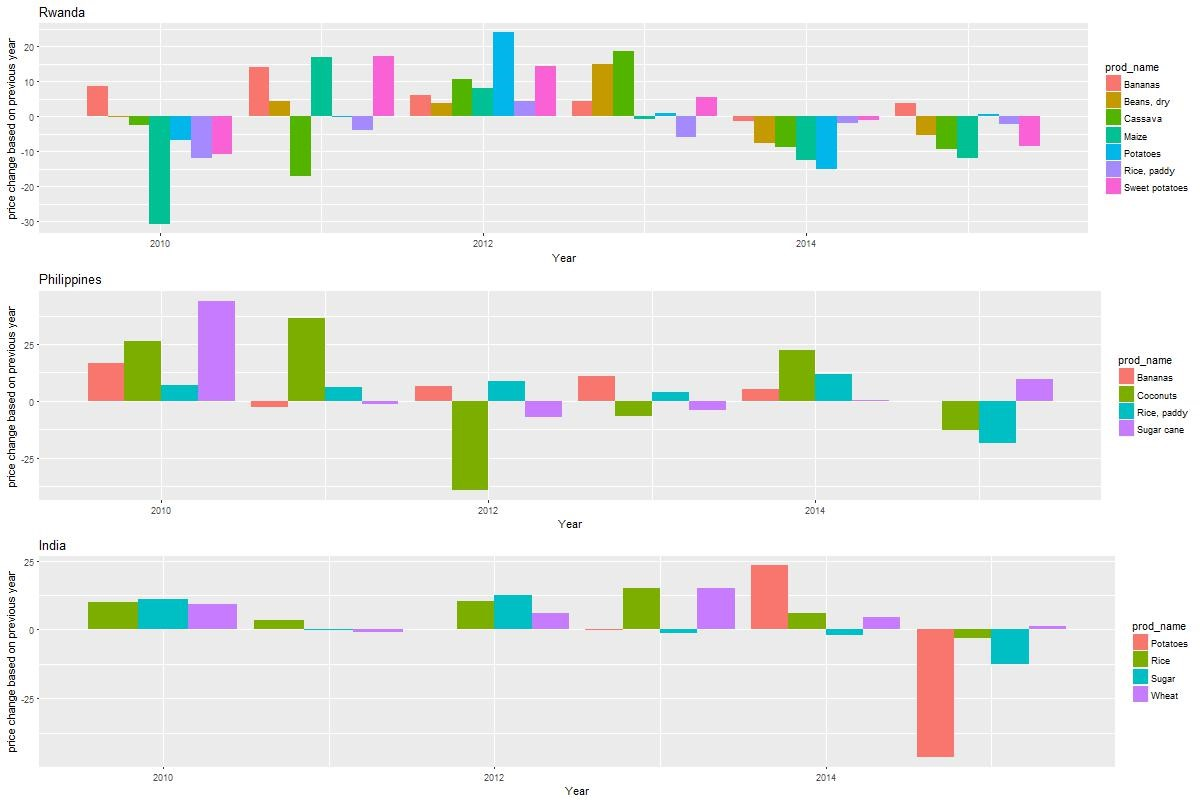
\includegraphics[scale=0.80]{barplot_price_change.jpg}
\caption{Products Price Change Based on The Cahnge from Previous Year }
\label{figure2}
\end{center}
\end{sidewaysfigure}
\FloatBarrier
The first graph \textbf{Figure 2} showcases the annual percentage price change of our crop selection.  Our selection is based on Harmonized System Codes (HS Code 2017). We focused on the category 07-015 – "Vegetables And Certain Roots And Tubers; Edible". 

\FloatBarrier
\begin{figure}[!htb]
\begin{center}
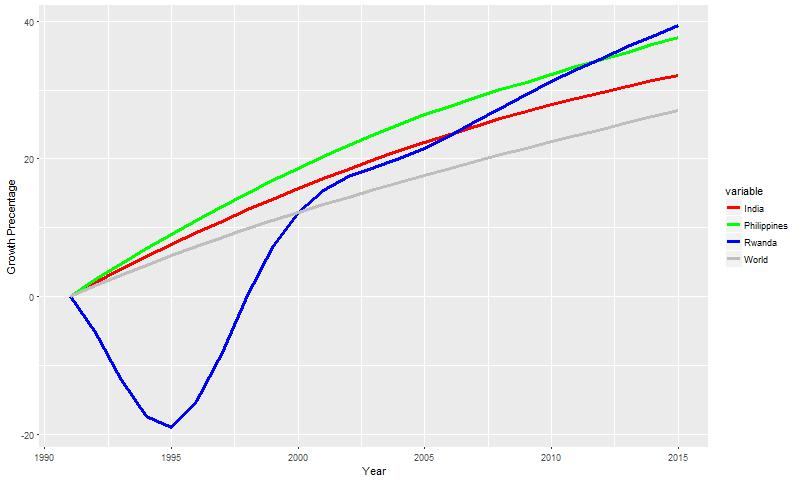
\includegraphics[scale=0.65]{population_plot.jpg}
\caption{Population Change}
\label{figure3}
\end{center}
\end{figure}
\FloatBarrier

The second graph \textbf{Figure 3} shows the population percentage population growth against the baseline world population percentage growth from 1990 to 2015. It is interesting to note that our country selection generally had a higher growth percentage than the global percentage trend with the notable outlier of Rwanda in the early 1990s. We assume that this sharp decline was related to the catastrophic civil war that ravaged Rwanda in 1994. 

\FloatBarrier
\begin{figure}[!htb]
\begin{center}
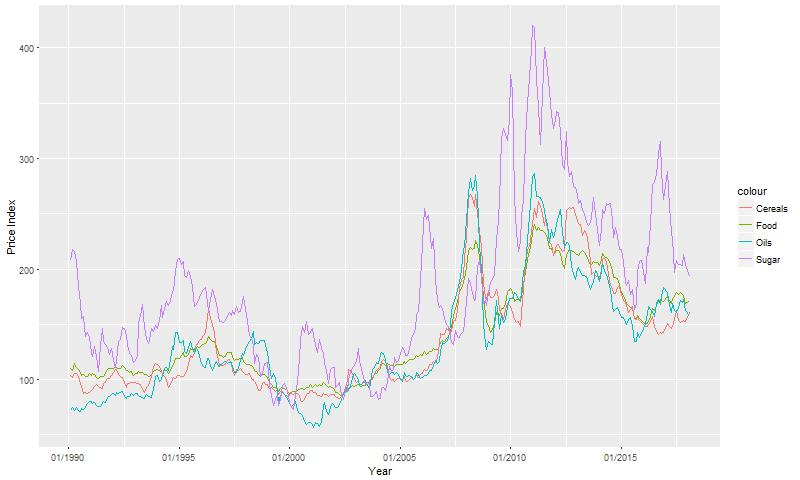
\includegraphics[scale=0.65]{price_index.jpg}
\caption{Global Avarage Food Category Price Change}
\label{figure4}
\end{center}
\end{figure}
\FloatBarrier

The next graph \textbf{Figure 4} shows the price index percentage change of cereals, vegetable oils and sugar against the global food price index percentage change from 1990 to 2015. A general upward trend can be observed with short term price spikes. Around 2010 a general price index drop can be observed. Sugar price percentage change is higher than the more homogenous trend development of cereals and vegetable oils which seem to be in line with the global food price index trend. These observations are in line with observations presented by the OECD. 

\FloatBarrier
\begin{sidewaysfigure}[!htb]
\begin{center}
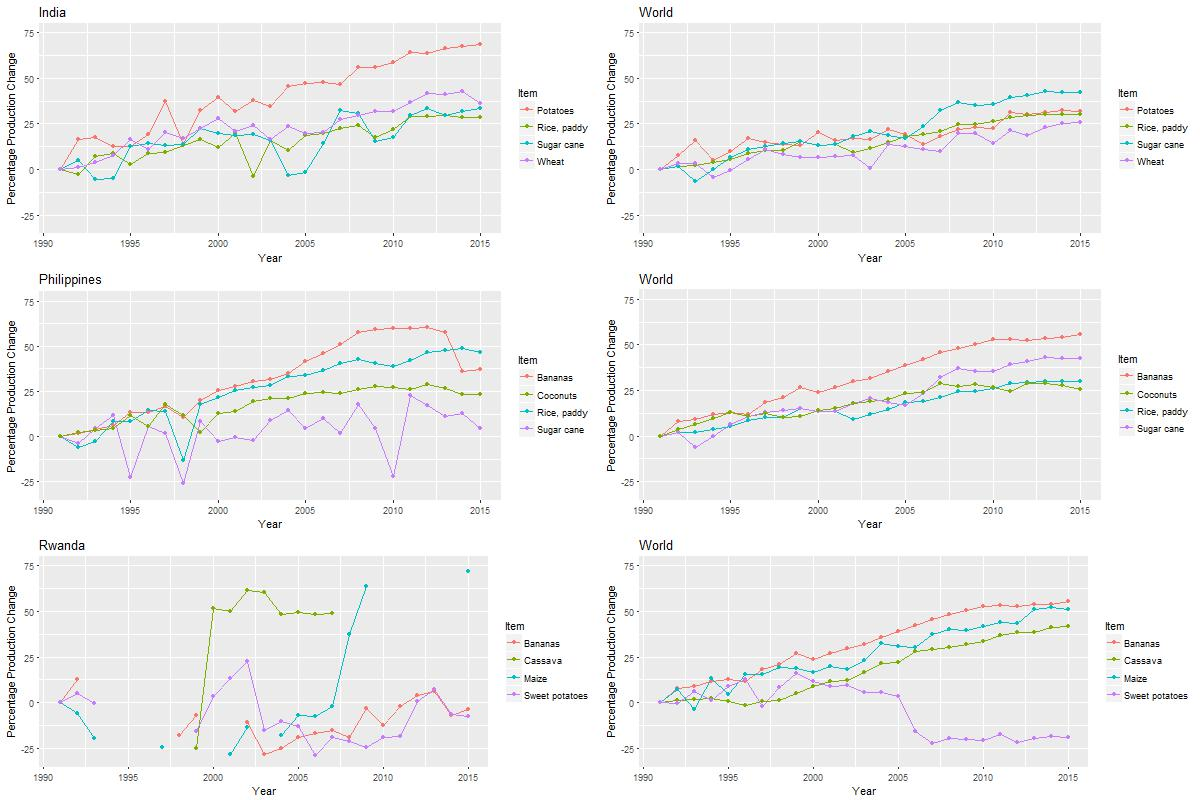
\includegraphics[scale=0.65]{production.jpg}
\caption{Consumer Price Development}
\label{figure5}
\end{center}
\end{sidewaysfigure}
\FloatBarrier

The final set of graphs \textbf{Figure 5} shows the consumer price development of our selected goods on a by country level against global consumer price development for the same goods from 1990 - 2015. Starting with India one can note that the general increasing global trend of consumer prices can be observed on the country level as well. Notable exceptions are the substantially higher consumer price development of potatoes as well as sharp price drops of rice and sugar in the early to mid 2000s. 
The Philippines are similar to India in the sense that the selected product consumer prices seem to follow the general global upward trend. The consumer price increase of Bananas, Coconuts and Rice are above the global trend. The notable exception is sugar which has quite volatile trend with multiple sharp consumer price drops. 
Rwanda is interesting as its consumer price trend is erratic in comparison to the global generally increasing trend. The global consumer food price for Bananas, Cassava and Maize increase at a constant rate whereas sweet potatoes seem to decrease and stagnate globally around 2005. The Rwandan consumer price for the same goods is in a sharp decline starting in the early 1990s, again our assumption is that this decline is related to the Rwandan civil war. A strong increase in consumer prices can be noted starting in the mid 1990s, spearheaded by Cassava and Maize consumer price development. 


\subsection{Results}

\subsubsection{Correlation / VIF based method}

\paragraph{4.2.1.1. Correlation overview}
The first step of this approach was to get an overview of pairwise correlations for each country’s dataset, measured by pearson’s correlation coefficient.

\FloatBarrier
\begin{figure}[!htb]
\begin{center}
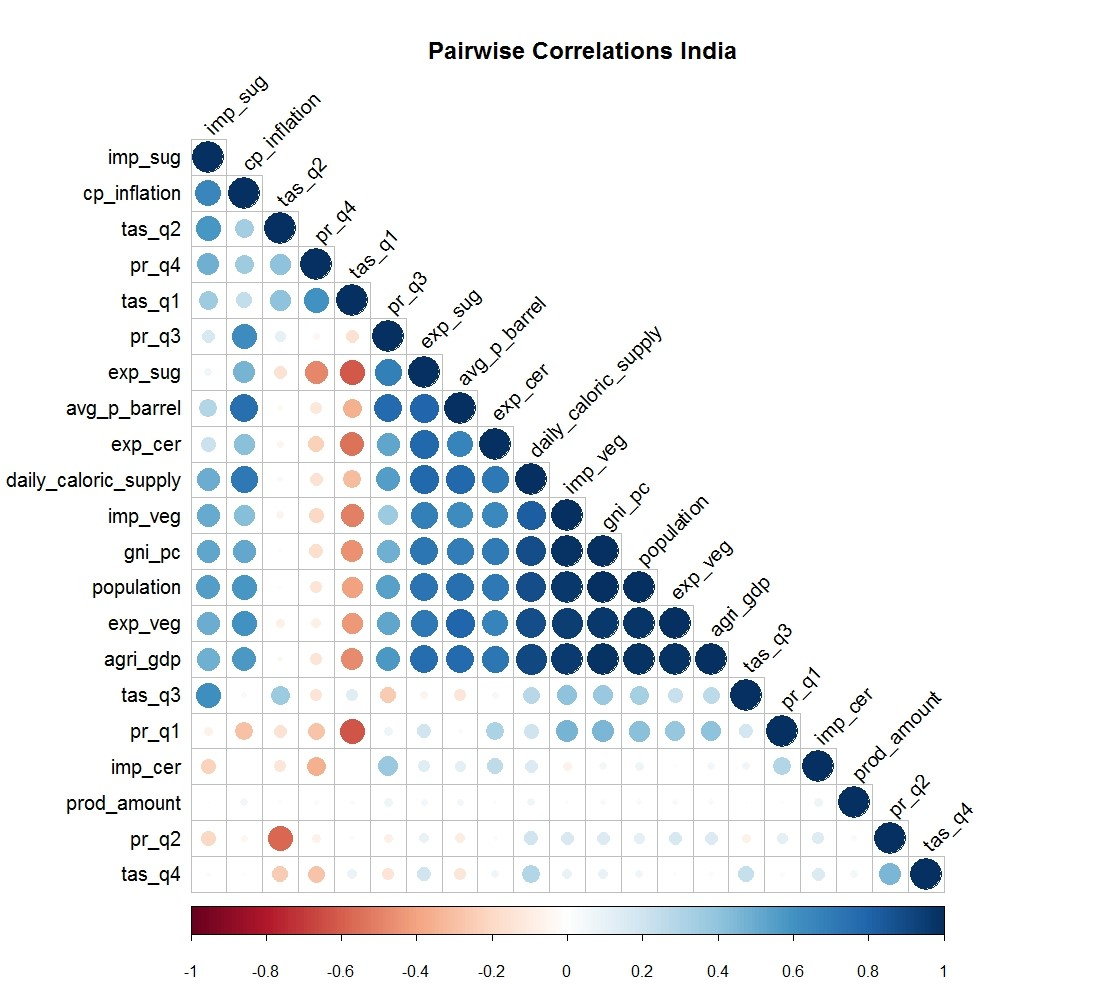
\includegraphics[scale=0.5]{R1.jpg}
\caption{India Correlations}
\label{figure6}
\end{center}
\end{figure}
\FloatBarrier

\FloatBarrier
\begin{figure}[!htb]
\begin{center}
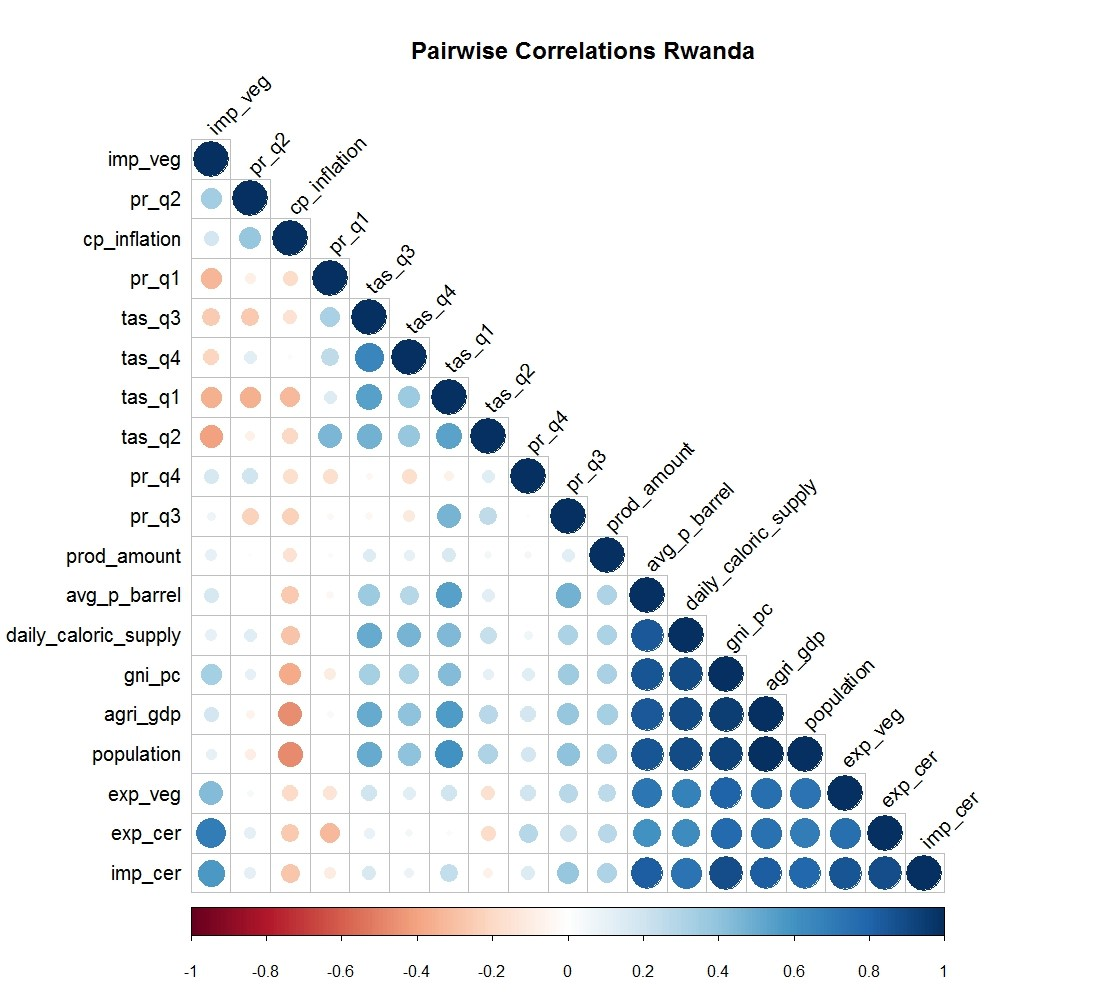
\includegraphics[scale=0.5]{R2.jpg}
\caption{Rwanda Correlations}
\label{figure7}
\end{center}
\end{figure}
\FloatBarrier

\FloatBarrier
\begin{figure}[!htb]
\begin{center}
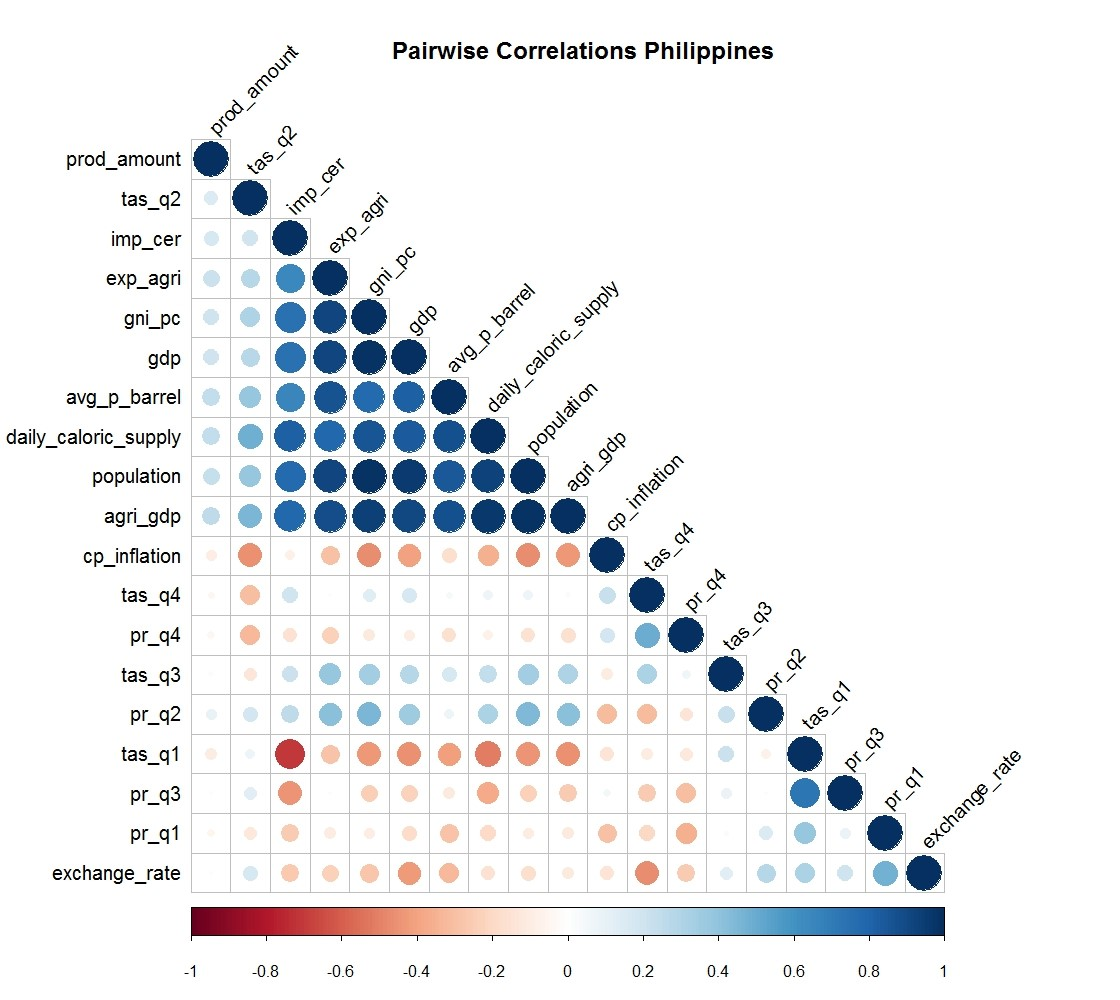
\includegraphics[scale=0.5]{R3.jpg}
\caption{Philippines Correlations}
\label{figure8}
\end{center}
\end{figure}
\FloatBarrier

\newpage
Variables which are part of a correlation pair with coefficient $>= 0.70$:

\FloatBarrier
\begin{table}[!htbp]
\centering
\begin{tabular}{lll}
{\ul India}            & {\ul Rwanda}           & {\ul Philippines}      \\
gni\_pc                & gni\_pc                & gni\_pc                \\
agri\_gdp              & agri\_gdp              & agri\_gdp              \\
population             & population             & population             \\
daily\_caloric\_supply & daily\_caloric\_supply & daily\_caloric\_supply \\
exp\_veg               & imp\_cer               & imp\_cer               \\
exp\_sug               & exp\_cer               & exp\_agri              \\
avg\_p\_barrel         & avg\_p\_barrel         & gdp                    \\
                       &                        & tas\_q1               
\end{tabular}
\caption{Correlations Variables}
\label{table6}
\end{table}
\FloatBarrier

\paragraph{4.2.1.2. Linear Model without highly correlated variables}

Having removed highly correlated variables, a linear model is built from the remaining predictors:
\begin{center}\underline{India}\\ \end{center}
\underline{Residuals:}
\begin{table}[!htbp]
\centering

\begin{tabular}{lllll}
Min      & 1Q       & Median  & 3Q      & Max     \\
-0.68000 & -0.23519 & 0.03321 & 0.22750 & 0.65974
\end{tabular}
\caption{India Residuals}
\label{table7}
\end{table}

\underline{Coefficients:}
\FloatBarrier
\begin{table}[!htbp]
\centering
\begin{tabular}{llllll}
\hline
Variable      & Estimate  & Std. Error & t value & Pr(\textgreater$|t|$) & Significant \\ \hline
(Intercept)   & -4.83E-12 & 4.95E+01   & 0.000   & 1.000             &             \\
pr\_q1        & -5.53E+02 & 3.19E+02   & -1.731  & 0.09243             & x           \\
pr\_q2        & -1.28E+02 & 1.00E+02   & -1.272  & 0.21217             &             \\
pr\_q3        & -2.23E+02 & 2.37E+02   & -0.944  & 0.35176             &             \\
pr\_q4        & 2.42E+02  & 2.28E+02   & 1.063   & 0.29506             &             \\
tas\_q1       & -5.04E+02 & 3.24E+02   & -1.554  & 0.12950             &             \\
tas\_q2       & 2.77E+02  & 2.06E+02   & 1.347   & 0.18686             &             \\
tas\_q3       & -5.31E+02 & 5.90E+02   & -0.900  & 0.37424             &             \\
tas\_q4       & 1.66E+02  & 1.22E+02   & 1.360   & 0.18283             &             \\
prod\_amount  & 6.34E+02  & 5.05E+01   & 12.561  & 2.52e-14            & x           \\
exp\_cer      & -3.41E+02 & 2.34E+02   & -1.455  & 0.15482             &             \\
imp\_sug      & 4.49E+02  & 6.66E+02   & 0.673   & 0.50548             &             \\
imp\_veg      & 1.21E+03  & 3.64E+02   & 3.316   & 0.00218             & x           \\
imp\_cer      & 5.62E+02  & 4.02E+02   & 1.396   & 0.17184             &             \\
cp\_inflation & -3.04E+02 & 3.71E+02   & -0.820  & 0.41774             &            \\ \hline
\end{tabular}
\caption{India Coefficients}
\label{table8}
\end{table}
\FloatBarrier
Residual standard error: 0.3466 on 34 degrees of freedom\\
Multiple R-squared:  0.9149, Adjusted R-squared:  0.8799 \\
F-statistic: 26.12 on 14 and 34 DF,  p-value: 3.915e-14

\newpage
\begin{center} \underline{Rwanda}\\ \end{center}
\underline{Residuals:}
\FloatBarrier
\begin{table}[!htbp]
\centering

\begin{tabular}{lllll}
Min     & 1Q      & Median  & 3Q     & Max    \\
-1.4427 & -0.6418 & -0.2439 & 0.3527 & 2.8037
\end{tabular}
\caption{Rwanda Residuals}
\label{table9}
\end{table}
\FloatBarrier

\underline{Coefficients:}
\FloatBarrier
\begin{table}[!htbp]
\centering
\begin{tabular}{llllll}
\hline
Variable      & Estimate  & Std. Error & t value & Pr(\textgreater$|t|$) & Significant \\ \hline
(Intercept)   & -9.63E-13 & 6.98E+01   & 0       & 1.00000             &             \\
pr\_q1        & 1.18E+02  & 8.92E+01   & 1.327   & 0.18638             &             \\
pr\_q2        & 9.90E+01  & 1.01E+02   & 0.98    & 0.3287              &             \\
pr\_q3        & 3.38E+01  & 1.01E+02   & 0.335   & 0.73769             &             \\
pr\_q4        & 1.01E+02  & 8.75E+01   & 1.151   & 0.25153             &             \\
tas\_q1       & 2.77E+02  & 1.20E+02   & 2.318   & 0.0217              & x           \\
tas\_q2       & -1.28E+02 & 1.19E+02   & -1.077  & 0.28327             &             \\
tas\_q3       & -1.79E+01 & 1.29E+02   & -0.139  & 0.88996             &             \\
tas\_q4       & 1.25E+02  & 1.11E+02   & 1.125   & 0.26234             &             \\
prod\_amount  & -2.19E+02 & 7.39E+01   & -2.959  & 0.00355             & x           \\
exp\_veg      & 1.26E+02  & 1.02E+02   & 1.234   & 0.21882             &             \\
imp\_veg      & 2.64E+02  & 1.00E+02   & 2.643   & 0.00903             & x           \\
cp\_inflation & -6.56E+01 & 8.64E+01   & -0.759  & 0.44901             &            \\ \hline
\end{tabular}
\caption{Rwanda Coefficients}
\label{table10}
\end{table}
\FloatBarrier

Residual standard error: 0.9235 on 162 degrees of freedom\\
Multiple R-squared:  0.2059, Adjusted R-squared:  0.1471 \\
F-statistic: 3.501 on 12 and 162 DF,  p-value: 0.0001285

\newpage

\begin{center} \underline{Philippines:} \\ \end{center}
\underline{Residuals:}
\FloatBarrier
\begin{table}[!htbp]
\begin{tabular}{lllll}
Min     & 1Q      & Median  & 3Q     & Max    \\
-0.9879 & -0.4897 & -0.2891 & 0.3079 & 2.4465
\end{tabular}
\centering
\caption{Philippines Residuals}
\label{table11}
\end{table}
\FloatBarrier

\underline{Coefficients:}
\FloatBarrier
\begin{table}[!htbp]
\centering
\begin{tabular}{llllll}
\hline
Variable       & Estimate  & Std. Error & t value & Pr(\textgreater$|t|$) & Significant \\ \hline
(Intercept)    & -1.10E-13 & 1.02E+02   & 0       & 1.00000             &             \\
tas\_q2        & -5.72E+01 & 1.65E+02   & -0.346  & 0.73059             &             \\
tas\_q3        & -1.15E+01 & 1.49E+02   & -0.077  & 0.93899             &             \\
tas\_q4        & 9.71E+01  & 1.67E+02   & 0.583   & 0.56205             &             \\
pr\_q1         & -1.01E+01 & 1.59E+02   & -0.064  & 0.94933             &             \\
pr\_q2         & 1.95E+02  & 1.22E+02   & 1.607   & 0.11324             &             \\
pr\_q3         & 8.93E+00  & 1.18E+02   & 0.076   & 0.93986             &             \\
pr\_q4         & -4.00E+01 & 1.43E+02   & -0.279  & 0.78124             &             \\
avg\_p\_barrel & 4.28E+02  & 1.44E+02   & 2.978   & 0.00419             & x           \\
prod\_amount   & -3.63E+02 & 1.07E+02   & -3.389  & 0.00124             & x           \\
exchange\_rate & -1.71E+02 & 1.69E+02   & -1.011  & 0.31585             &             \\
cp\_inflation  & -1.09E+02 & 1.45E+02   & -0.750  & 0.45605             &            \\ \hline
\end{tabular}
\caption{Philippines Coefficients}
\label{table12}
\end{table}
\FloatBarrier
Residual standard error: 0.8693 on 60 degrees of freedom \\
Multiple R-squared:  0.3614,	Adjusted R-squared:  0.2444 \\ 
F-statistic: 3.087 on 11 and 60 DF,  p-value: 0.002419 \\

\newpage
\paragraph{4.2.1.3. Linear Model with variables left after VIF-removal}

Since removing highly correlated variables leads to some potentially important variables being dropped, we applied VIF-removal to both the set of highly correlated variables and the remaining set.
Creating another linear model with the resulting set of variables we obtained the following results

\begin{center}\underline{India:} \end{center}
\underline{Residuals:}
\FloatBarrier
\begin{table}[!htbp]
\centering
\begin{tabular}{lllll}
Min      & 1Q       & Median  & 3Q      & Max     \\
-0.66068 & -0.22061 & 0.02824 & 0.20910 & 0.67543
\end{tabular}
\caption{India Residuals}
\label{table13}
\end{table}
\FloatBarrier

\underline{Coefficients:}
\FloatBarrier
\begin{table}[!htbp]
\centering
\begin{tabular}{llllll}
\hline
                       & Estimate  & Std. Error & t value & Pr(\textgreater$|t|$) & Significant \\ \hline
(Intercept)            & 4.16E-12  & 5.00E+01   & 0       & 1.0000              &             \\
population             & 1.41E+03  & 6.42E+02   & 2.188   & 0.0359              & x           \\
daily\_caloric\_supply & -4.90E+02 & 1.01E+03   & -0.486  & 0.6301              &             \\
exp\_sug               & 2.41E+03  & 2.54E+03   & 0.948   & 0.3501              &             \\
avg\_p\_barrel         & -3.99E+02 & 8.40E+02   & -0.475  & 0.6379              &             \\
pr\_q1                 & -2.76E+02 & 1.69E+02   & -1.634  & 0.1118              &             \\
pr\_q2                 & -5.54E+02 & 5.53E+02   & -1.002  & 0.3236              &             \\
pr\_q3                 & -1.18E+03 & 1.05E+03   & -1.130  & 0.2667              &             \\
pr\_q4                 & 1.31E+03  & 1.12E+03   & 1.172   & 0.2494              &             \\
tas\_q2                & -2.57E+02 & 5.92E+02   & -0.435  & 0.6667              &             \\
tas\_q3                & 2.03E+01  & 2.90E+02   & 0.070   & 0.9448              &             \\
tas\_q4                & -1.64E+02 & 2.40E+02   & -0.682  & 0.5001              &             \\
prod\_amount           & 6.34E+02  & 5.10E+01   & 12.418  & 5.51e-14            & x           \\
exp\_cer               & -9.57E+02 & 8.72E+02   & -1.097  & 0.2806              &             \\
imp\_cer               & 8.96E+02  & 8.99E+02   & 0.996   & 0.3264              &             \\
cp\_inflation          & -2.06E+02 & 6.71E+02   & -0.307  & 0.7604              &            \\ \hline
\end{tabular}
\caption{India Coefficients}
\label{table14}
\end{table}
\FloatBarrier
Residual standard error: 0.35 on 33 degrees of freedom \\
Multiple R-squared:  0.9158,	Adjusted R-squared:  0.8775 \\ 
F-statistic: 23.92 on 15 and 33 DF,  p-value: 1.758e-13

\newpage

\begin{center}\underline{Rwanda} \end{center}
\underline{Residuals:}
\FloatBarrier
\begin{table}[!htbp]
\centering
\begin{tabular}{lllll}
Min     & 1Q      & Median  & 3Q     & Max    \\
-1.5524 & -0.6039 & -0.2119 & 0.3888 & 2.9797
\end{tabular}
\caption{Rwanda Residuals}
\label{table15}
\end{table}
\FloatBarrier

\underline{Coefficients:} \\

\FloatBarrier
\begin{table}[!htbp]
\centering
\begin{tabular}{llllll}
\hline
                       & Estimate  & Std. Error & t value & Pr(\textgreater$|t|$) & Significant \\ \hline
(Intercept)            & -6.61E-13 & 6.91E+01   & 0       & 1.00000             &             \\
population             & 5.28E+02  & 4.79E+02   & 1.102   & 0.27214             &             \\
daily\_caloric\_supply & -4.03E+02 & 2.85E+02   & -1.413  & 0.15966             &             \\
avg\_p\_barrel         & 3.42E+02  & 1.81E+02   & 1.892   & 0.06027             & x           \\
exp\_cer               & -1.72E+01 & 2.91E+02   & -0.059  & 0.9531              &             \\
pr\_q1                 & 1.35E+02  & 1.00E+02   & 1.348   & 0.17956             &             \\
pr\_q2                 & 1.21E+02  & 1.40E+02   & 0.867   & 0.38741             &             \\
pr\_q3                 & 1.44E+01  & 1.15E+02   & 0.125   & 0.90036             &             \\
pr\_q4                 & 8.60E+01  & 1.02E+02   & 0.84    & 0.40223             &             \\
tas\_q1                & 2.73E+01  & 1.88E+02   & 0.146   & 0.88442             &             \\
tas\_q2                & -1.56E+02 & 1.29E+02   & -1210   & 0.22816             &             \\
tas\_q3                & 2.02E+01  & 1.59E+02   & 0.127   & 0.89905             &             \\
tas\_q4                & 9.00E+01  & 1.18E+02   & 0.761   & 0.44762             &             \\
prod\_amount           & -2.31E+02 & 7.38E+01   & -3131   & 0.00208             & x           \\
exp\_veg               & -1.30E+02 & 1.57E+02   & -0.831  & 0.4075              &             \\
imp\_veg               & 2.09E+02  & 1.77E+02   & 1.180   & 0.2397              &             \\
cp\_inflation          & 2.12E+01  & 1.08E+02   & 0.196   & 0.8446              &            \\ \hline
\end{tabular}
\caption{Rwanda Coefficients}
\label{table16}
\end{table}
\FloatBarrier
Residual standard error: 0.9138 on 158 degrees of freedom \\
Multiple R-squared:  0.2417,	Adjusted R-squared:  0.1649 \\
F-statistic: 3.148 on 16 and 158 DF,  p-value: 0.0001125

\newpage
\begin{center}\underline{Philippines} \end{center}
\underline{Residuals:}
\FloatBarrier
\begin{table}[!htbp]
\centering
\begin{tabular}{lllll}
Min     & 1Q      & Median  & 3Q     & Max    \\
-1.0930 & -0.4379 & -0.2995 & 0.2246 & 2.3262
\end{tabular}
\caption{Philippines Residuals}
\label{table17l}
\end{table}
\FloatBarrier

\underline{Coefficients:}
\FloatBarrier
\begin{table}[!htbp]
\centering
\begin{tabular}{llllll}
\hline
                       & Estimate  & Std. Error & t value & Pr(\textgreater$|t|$) & Significant \\ \hline
(Intercept)            & -1.14E-13 & 1.05E+02   & 0       & 1.00000             &             \\
daily\_caloric\_supply & 4.35E+02  & 1.26E+03   & 0.346   & 0.7308              &             \\
exp\_agri              & 3.70E+02  & 6.26E+02   & 0.591   & 0.55687             &             \\
imp\_cer               & -7.12E+01 & 5.27E+02   & -0.135  & 0.89303             &             \\
tas\_q1                & -1.98E+02 & 3.95E+02   & -0.502  & 0.61793             &             \\
tas\_q2                & -3.10E+01 & 2.90E+02   & -0.107  & 0.91522             &             \\
tas\_q3                & -1.15E+01 & 2.58E+02   & -0.044  & 0.96469             &             \\
tas\_q4                & 4.17E+01  & 1.86E+02   & 0.225   & 0.82314             &             \\
pr\_q1                 & 2.46E+01  & 2.58E+02   & 0.095   & 0.92448             &             \\
pr\_q2                 & -4.54E+01 & 3.47E+02   & -0.131  & 0.89644             &             \\
pr\_q3                 & 1.92E+02  & 3.11E+02   & 0.619   & 0.53835             &             \\
pr\_q4                 & -1.47E+01 & 2.45E+02   & -0.060  & 0.95243             &             \\
avg\_p\_barrel         & -2.64E+02 & 1.19E+03   & -0.222  & 0.8252              &             \\
prod\_amount           & -3.64E+02 & 1.10E+02   & -3.316  & 0.00161             & x           \\
exchange\_rate         & -2.01E+02 & 2.25E+02   & -0.894  & 0.3754              &             \\
cp\_inflation          & -6.22E+01 & 1.96E+02   & -0.317  & 0.7523              &            \\ \hline
\end{tabular}
\caption{Philippines Coefficients}
\label{table18}
\end{table}
\FloatBarrier
Residual standard error: 0.8884 on 56 degrees of freedom \\
Multiple R-squared:  0.3775,	Adjusted R-squared:  0.2108 \\ 
F-statistic: 2.264 on 15 and 56 DF,  p-value: 0.01414

\newpage
\subsubsection{Lasso based method}

Note: the left dotted line indicates the lambda leading to the model with minimal mse, which we chose as a base for variable selection. The right dotted line shows points at the lambda leading to a model for which the error is within one standard error of the minimum

\FloatBarrier
\begin{figure}[!htb]
\begin{center}
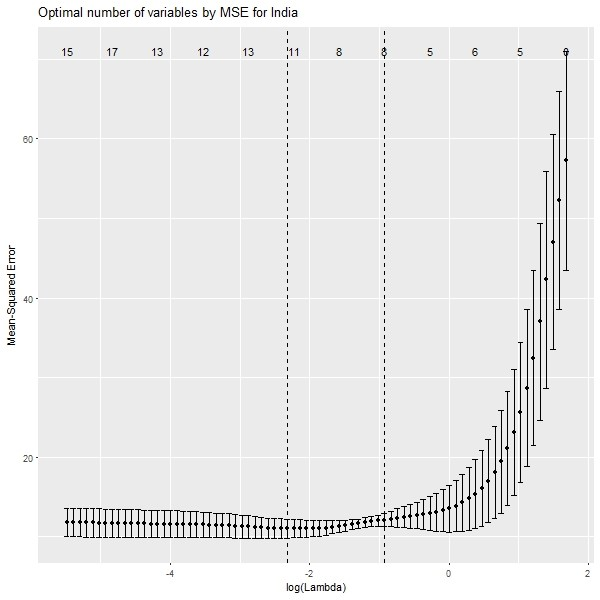
\includegraphics[scale=0.85]{L1.jpg}
\caption{India Optimal Number of Variables}
\label{figure9}
\end{center}
\end{figure}
\FloatBarrier

Important variables for India:

\FloatBarrier
\begin{table}[!htbp]
\begin{tabular}{lll}
\hline
{\ul variables}        & {\ul coefs\_minlambda} & {\ul colors} \\ \hline
tas\_q2                & 8.203321e-01           & green        \\
prod\_amount           & 4.289088e-05           & green        \\
exp\_veg               & 2.596261e-06           & green        \\
agri\_gdp              & 5.487558e-11           & green        \\
exp\_cer               & 7.872368e-11           & green        \\
imp\_sug               & 7.540223e-07           & green        \\
imp\_veg               & 2.962602e-07           & green        \\
imp\_cer               & -2.776436e-06          & red          \\
pr\_q2                 & -2.285270e-02          & red          \\
pr\_q1                 & -1.124898e-02          & red          \\
tas\_q3                & 8.462011e-01           & green       \\ \hline
\end{tabular}
\centering
\caption{Important variables for India}
\label{table19}
\end{table}
\FloatBarrier


\FloatBarrier
\begin{figure}[!htb]
\begin{center}
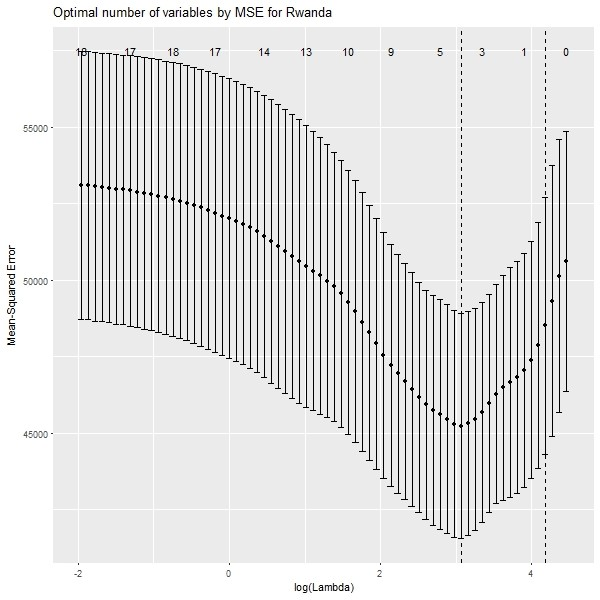
\includegraphics[scale=0.85]{L2.jpg}
\caption{Rwanda Optimal Number of Variables}
\label{figure10}
\end{center}
\end{figure}
\FloatBarrier

Important variables for Rwanda:

\FloatBarrier
\begin{table}[!htbp]
\centering
\begin{tabular}{lll}
\hline
{\ul variables}        & {\ul coefs\_minlambda} & {\ul colors} \\ \hline
tas\_q4                & 1.543063e+00           & green        \\
avg\_p\_barrel         & 1.855989e-01           & green        \\
imp\_cer               & 1.654824e-03           & green        \\
prod\_amount           & -2.160013e-05          & red          \\  \hline
\end{tabular}
\caption{Important variables for Rwanda}
\label{table20}
\end{table}
\FloatBarrier

\FloatBarrier
\begin{figure}[!htb]
\begin{center}
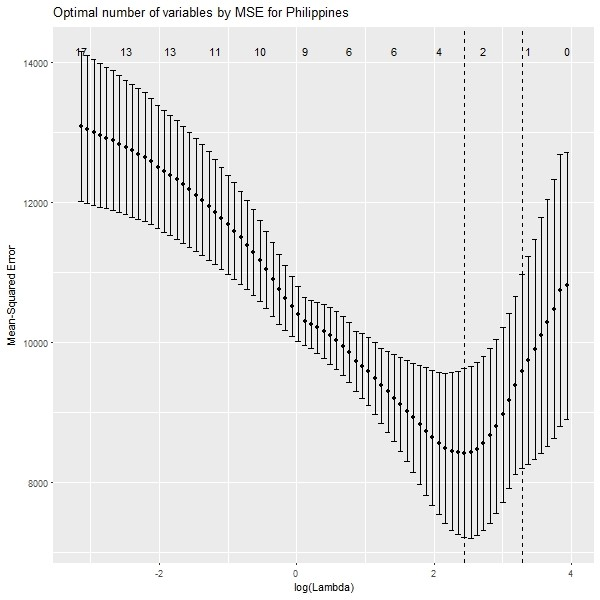
\includegraphics[scale=0.85]{L3.jpg}
\caption{Philippines Optimal Number of Variables}
\label{figure11}
\end{center}
\end{figure}
\FloatBarrier

Important variables for Philippines:

\FloatBarrier
\begin{table}[!htbp]
\centering
\begin{tabular}{ll}
\hline
{\ul variables} & {\ul coefs\_minlambda} \\ \hline
gdp             & 5.429905e-10           \\
prod\_amount    & -3.595559e-06          \\
avg\_p\_barrel  & 8.018443e-02          \\ \hline
\end{tabular}
\caption{Important variables for Philippines}
\label{table21}
\end{table}
\FloatBarrier

\newpage
\subsubsection{Random Forest based method}

\FloatBarrier
\begin{figure}[!htb]
\begin{center}
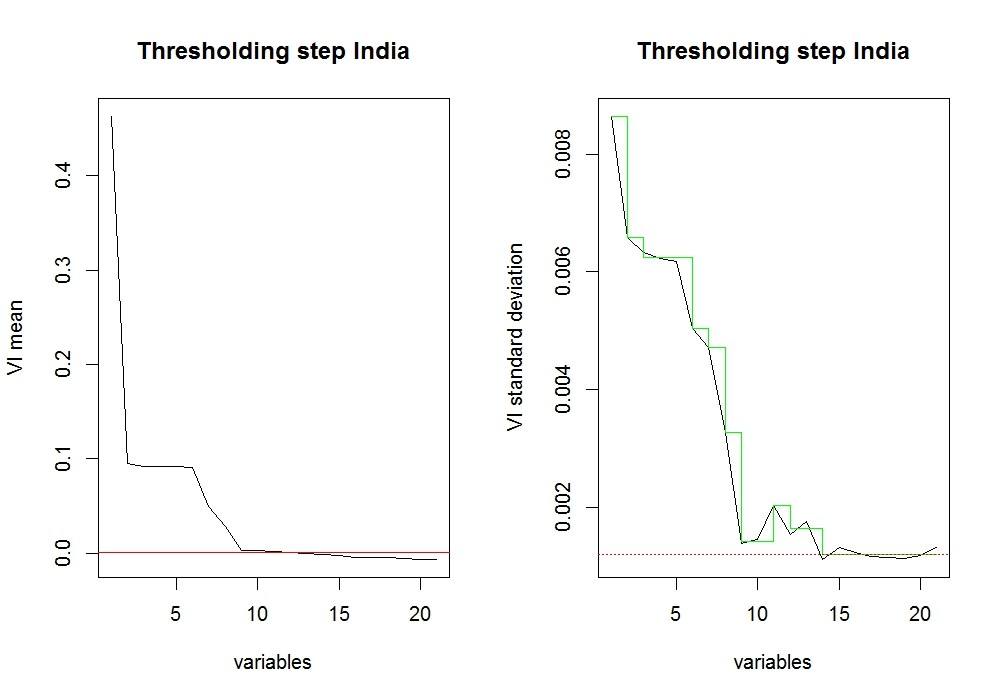
\includegraphics[scale=0.55]{F1.jpg}
\caption{India Thresholding Step}
\label{figure12}
\end{center}
\end{figure}
\FloatBarrier

\FloatBarrier
\begin{figure}[!htb]
\begin{center}
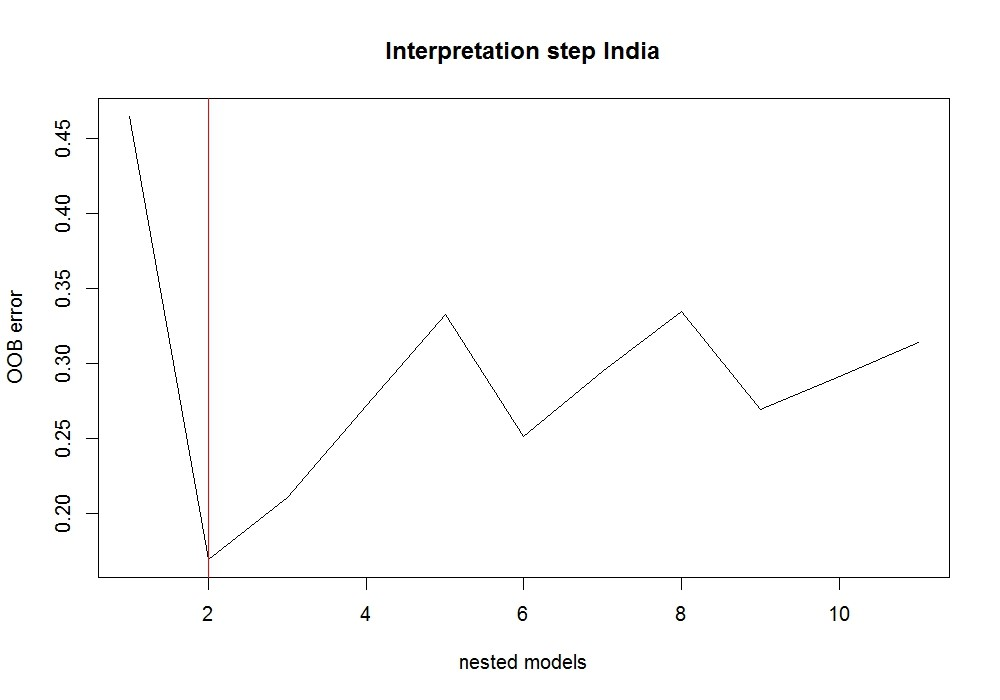
\includegraphics[scale=0.55]{F2.jpg}
\caption{India interpretation Step }
\label{figure13}
\end{center}
\end{figure}
\FloatBarrier

\FloatBarrier
\begin{figure}[!htb]
\begin{center}
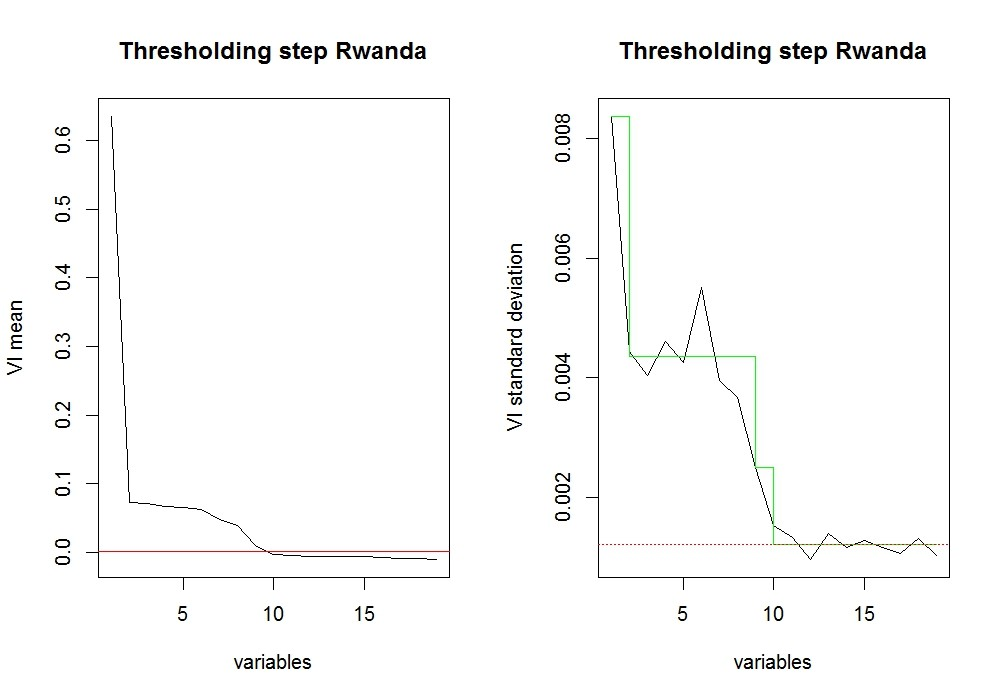
\includegraphics[scale=0.55]{F3.jpg}
\caption{Rwanda Thresholding Step}
\label{figure14}
\end{center}
\end{figure}
\FloatBarrier

\FloatBarrier
\begin{figure}[!htb]
\begin{center}
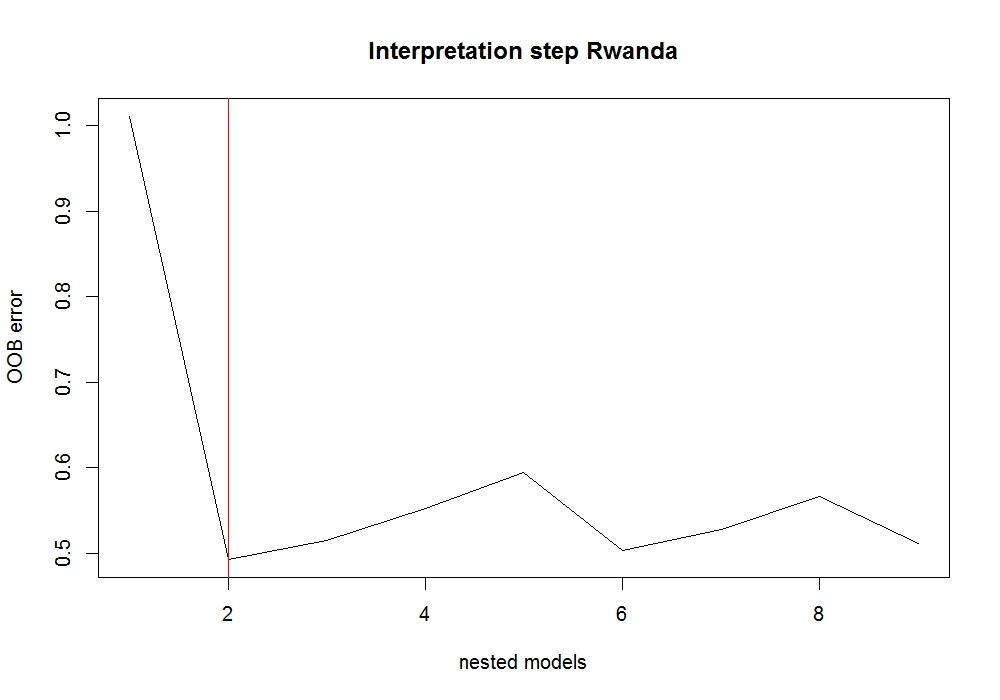
\includegraphics[scale=0.55]{F4.jpg}
\caption{Rwanda interpretation Step}
\label{figure15}
\end{center}
\end{figure}
\FloatBarrier

\FloatBarrier
\begin{figure}[!htb]
\begin{center}
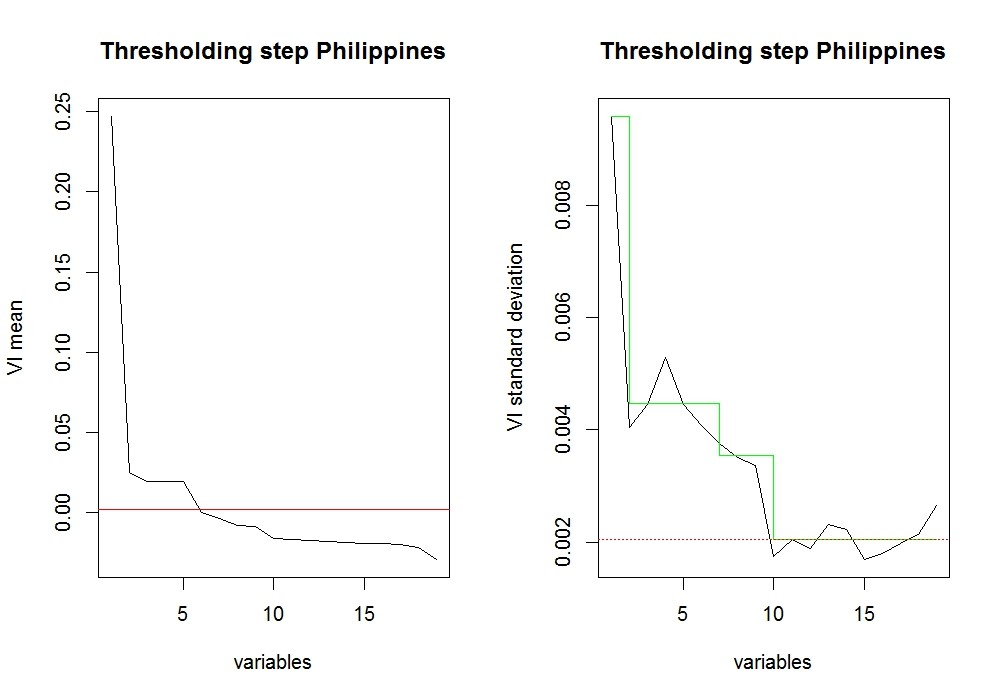
\includegraphics[scale=0.55]{F5.jpg}
\caption{Philippines Thresholding Step}
\label{figure16}
\end{center}
\end{figure}
\FloatBarrier

\FloatBarrier
\begin{figure}[!htb]
\begin{center}
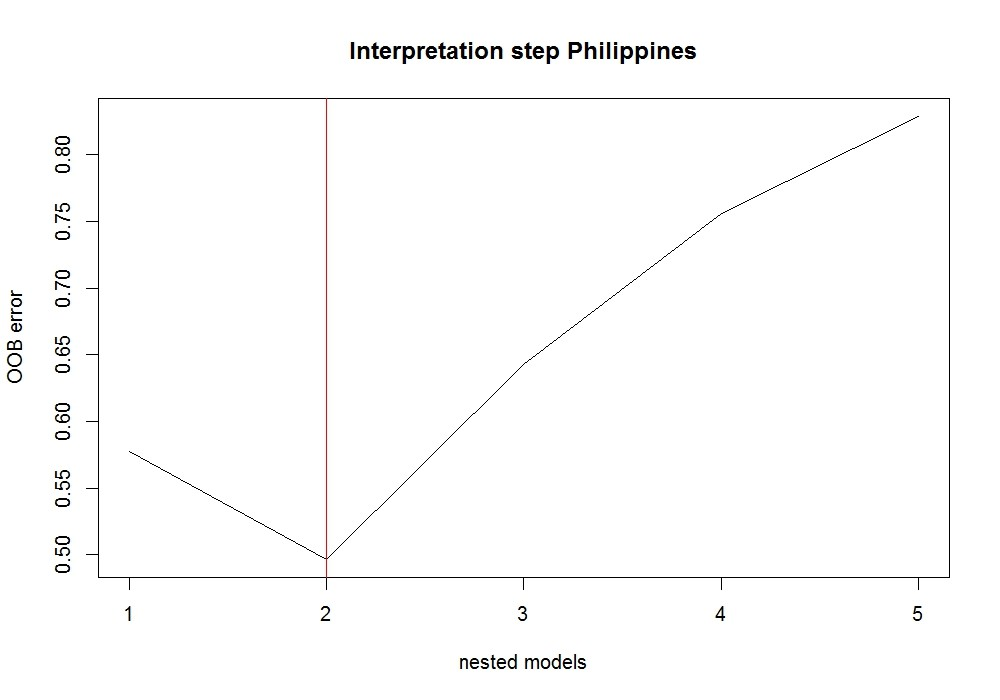
\includegraphics[scale=0.55]{F6.jpg}
\caption{Philippines interpretation Step}
\label{figure17}
\end{center}
\end{figure}
\FloatBarrier

\FloatBarrier
\begin{table}[!htbp]
\centering
\begin{adjustbox}{max width=\textwidth}
\begin{tabular}{llllll}
\hline 
\multicolumn{2}{l}{{\ul India}}                    & \multicolumn{2}{l}{{\ul Rwanda}}                   & \multicolumn{2}{l}{{\ul Philippines}}            \\ \hline
{\ul threshold step}   & {\ul interpretation step} & {\ul threshold step}   & {\ul interpretation step} & {\ul threshold step} & {\ul interpretation step} \\ 
prod\_amount           & prod\_amount              & prod\_amount           & prod\_amount              & prod\_amount         & prod\_amount              \\ 
agri\_gdp              & agri\_gdp                 & agri\_gdp              &                           & agri\_gdp            & agri\_gdp                 \\ 
gni\_pc                &                           & gni\_pc                &                           & gni\_pc              &                           \\ 
population             &                           & population             &                           & population           &                           \\  
imp\_veg               &                           &                        &                           &                      &                           \\  
exp\_veg               &                           & exp\_veg               &                           &                      &                           \\  
daily\_caloric\_supply &                           & daily\_caloric\_supply &                           &                      &                           \\  
imp\_sug               &                           &                        &                           &                      &                           \\  
cp\_inflation          &                           &                        &                           &                      &                           \\  
imp\_cer               &                           & imp\_cer               & imp\_cer                  &                      &                           \\ 
exp\_sug               &                           &                        &                           &                      &                           \\ 
                       &                           & exp\_cer               &                           &                      &                           \\ 
                       &                           & avg\_p\_barrel         &                           &                      &                           \\ 
                       &                           &                        &                           & gdp                  &                          \\ \hline
\end{tabular}
\end{adjustbox}
\caption{Random Forest Selection}
\label{table22}
\end{table}
\FloatBarrier

\subsubsection{Summary}

\begin{center} \underline{India:} \end{center}
The linear model with non highly correlated variables reveals that the amount of rain in the first quarter, the produced amount and the amount of imported vegetables significantly affect the price. 
The model made after VIF reduction has only two significant variables, population and produced amount. It appears that population, the only significant demand related factor , outweighs climatic and macroeconomic supply related factors in terms of predictive power in the linear models. However produced amount seems to be the most important factor since it is always included.

The lasso method gives a more differentiated impression.
Again, produced amount seems to be important. Imports of sugar, vegetables and cereals as well as demand related factors exports of vegetables and cereals also have an impact on price. Climatic factors play a bigger role here since rain in the first half of the year and temperatures from April to September also appear to be a driving factor, probably because of their impact on the agricultural output. The fact that agricultural GDP is also on the list supports this.

The findings produced by the threshold step of the RF method generally go in the same direction as produced amount and agri\_gdp seem to be important again as well as imports of sugar and vegetables and export of vegetables. In addition to that population size, gross national income per capita, daily caloric supply and inflation have an influence on price too. After the interpretation step only produced amount and agri\_gdp are left.

The importance of the produced amount is evident as it is included in every result. On the demand side, population size and food exports appear to be the most influencial factors. 

\begin{center} \underline{Rwanda:} \end{center}
According to the findings produced by the linear model with no highly correlated variables, only supply related factors are to be considered. Produced amount appears to be very important, temperature in the first quarter and the amount of imported vegetables are also influencial.
The VIF based model reveals that apart from produced amount, food prices in Rwanda are also dependent on the petrol oil price. 
These findings are support by the results of the lasso model, as in addition to produced amount and oil price, rain in the fourth quarter of the year and the import of cereals are also an affecting food prices.

The RF model indicates, that in addition to agricultural output, demand related variables such as population size, GNI per capita, daily caloric supply and the amount of exported vegetables contribute to food price development. After the interpretation step only produced amount is left.

Again, the single most important factor appears to be produced amount. Combined with demographic factors and the dependency of Rwanda’s agriculture on petroleum most of the food prices in this country can be explained.

\begin{center} \underline{Philippines:} \end{center}

The linear model with low correlated variables for the Philippines gives only two significant factors : oil price per barrel and produced amount. The VIF based model only has produced amount.
While not adding any further information these findings are in line with the results for the other two countries.
This is also supported by the findings obtained from the lasso model, as only gdp, produced amount and oil price per barrel appear to be important.
The interpretation step of the RF model adds population and gni\_pc to the list of relevant variables, produced\_amount and agri\_gdp are considered important as well. After the interpretation step only produced amount and agri\_gdp remain.

In the Philippines, food prices appear to be mostly driven by the produced amount and the population, while other factors only play a minor role.


\section{Conclusion}
Erokhin highlighted the fact that one important contributing factor to food security are food prices in his work. The OECD identified an understanding on food price development as a paramount basis for sound food security policy decision making on the national level. With these observations in mind we started this work with the goal to see if we could replicate the findings of Erokhin and the OECD on a country specific level. The initial step was the country selection. We decided on India, Rwanda and the Philippines as this selection of countries provided us with a varied economic, political and climatic basis of research, which in turn allowed us to form a comprehensive conclusion if the global OECD findings were applicable on a country specific level. 
We will first contrast the global OECD findings on consumer food price development with the country specific selection of consumer goods food price development. All goods selected were chosen based on the Harmonized System Codes (HS Code 2017). We focused on the category 07-015. \\
The OECD analyzed annual consumer food price development of wheat, coarse grains rice and oil seeds from 1971 to 2007. The conclusion is that consumer food prices are volatile and price spikes are a common occurrence. The OECD has identified unfavorable climatic conditions in 2005 and 2007 in major crop producing regions as one factor contributing to an increase in consumer food prices (OECD, 2008). Further strong demand growth for food and animal feed led to increase in price development. Other factors contributing to consumer price trend development as noted by the OECD are the following: Macro-economic conditions such as GDP growth in developing countries and oil price development. The OECD predicted based on the above factors that global consumer food prices would increase in comparison to historic trends but also that consumer prices would decrease from the from 2007-2008 spike price level. \\
Our findings support this prediction as one can note a general upward trend in the global as well as national consumer food prices for our selection of goods as shown in section 4.1. Figure 2 shows that consumer prices of our selection of cereals, vegetables oils and sugar are increasing in accordance with global food consumer prices. One can observe that while this price development is above the historic trend and generally increasing, the price spike in 2007-2008 has normalized as predicted by the OECD. The different models used in the variable selection process gave some further insights in regard to which factors were most influential on consumer price development. Produced amount was the most influential supply side factor across all three countries. These findings are in accordance with OECD findings regarding demand development. The OECD further notes animal feed as driving demand factor, which is one limitation of our work as we have no data on life feed demand influences. Population growth was the most influential demand side factor for our country selection. Country specific difference in the influential factors could also be observed. Crop prices in the Philippines are mainly unaffected by any of the factors we considered apart from produced amount and population. India and Rwanda hat some interesting country specific influential factors. Climatic factors rain and temperature were important when looking at India, most likely as they influenced agricultural output. Further on a macro-economic level food exports were especially influential on price development in India. This in accordance with Erokhin's observation on food security being negatively influenced by an increase in exports. Food price development in Rwanda seems to hinge exponentially on oil price development. The OECD states oil price development as a price influencing factor but price development in Rwanda seems to be more influenced by oil price development than the global trend. Our findings show that the global perspective and prediction of the OECD in regards to the consumer food price index hold true on a by country level. \\
OECD stance on an increasing trend of consumer food prices in regards to food security is that while the overall impact on developing countries is modest, urban poor populations will be strongly negatively impacted. This discrepancy of modest national impact to strong negative impact for the poor urban population is based on the share of disposable income available and its use to purchase food at higher consumer food prices. According to Erokhin another negative aspect of an increase in consumer food prices is that exporting goods becomes more profitable to producers from countries with a weak local currency (Erokhin, 2017). This can further exacerbate food security for the poorest populations of a country. \\

It appears that for any of the countries that we considered, population growth and the amount of domestically produced crops have the highest impact on local food prices. Whether this also holds true for other countries, remains to be seen. In any case both of these factors deserve further inspection, particularly focusing on the reasons and mechanisms behind population growth and production amounts.



%\begin{thebibliography}{9}
%\bibitem{latexcompanion} Michel Goossens, Frank Mittelbach, and Alexander Samarin. \textit{The \LaTeX\ Companion}. Addison-Wesley, Reading, Massachusetts, 1993.
%\bibitem{Erokhin} Erokhin. \textit{V. Establishing Food Security and Alternatives to International Trade in Emerging Economies}.  Case of Adana. Pak. J. Nutr. 2013, 13, 1–6
%\end{thebibliography}

\newpage
\textbf{References} \hfill \break
\hfill \break
[1]. Food and Agriculture Organization of the United Nations. Food and Agriculture
Data. Available online: \url{http://faostat.fao.org/beta/en/#home} (accessed on 15th February 2017). \hfill \break
\hfill \break
[2]. Erokhin, V. Establishing Food Security and Alternatives to International Trade in
Emerging Economies; IGI Global: Hershey, PA, USA, 2017. \hfill \break
\hfill \break
[3] . Esturk, Oren, M.N. Impact of household socio-economic factors on food security: Case of Adana. Pak. J. Nutr. 2013, 13, 1–6. \hfill \break
\hfill \break
[4]. Smith, M.E. World Food Security. The Effect of U.S. Farm Policy; 
United States Department of Agriculture: Washington, WA, USA, 1990.  \hfill \break
\hfill \break
[5]. Bühlmann, Peter, and Sara van de Geer. Statistics for High-Dimensional Data: Methods, Theory and Applications. Springer, 2013. \hfill \break
\hfill \break
[6]. OECD, (2008). Rising Food Prices: Causes and Consequences. Organisation for Economic Co-operation and Development (OECD). \url{http://www.oecd.org/trade/agricultural-trade/40847088.pdf} Retrieved 14th January, 2018.



%\bibliographystyle{plain}
%\bibliography{biblist}
\newpage 

\textbf{Appendix} \hfill \break
\hfill \break
\begin{lstlisting}[language= R]
#this script shall load all final dataset files created in the preparation stage and include the code for displaying 
# eplorative graphs and tables.


# plotting the population for the all countries and the world
source(".\\Helper_functions\\exploration_functions.r")

if(!require("reshape2")) install.packages("reshape2");library("reshape2")
if(!require("ggplot2")) install.packages("ggplot2");library("ggplot2")
if(!require("data.table")) install.packages("data.table");library("data.table")
if(!require("zoo")) install.packages("zoo");library("zoo")


#reading the data  
world_population = read.csv(".\\Common_datasets\\world_population.csv", stringsAsFactors = FALSE, sep = ",", header = TRUE)

# stacks a set of columns into a single column of data to be able to process it 
world_population = melt(world_population, id=c("Year"), value.name = "population")

# calculating the percentage of the change in the population
for(i in unique(world_population$variable)){
  # i is the name of the land 
  #print(i)
  world_population = calcPercFixBaseyear(world_population,"variable",i,"Year",1991,"population", "percentage")
}

# creating and saving the plot
jpeg(".//Ds_overview_plots//population_plot.jpg", width = 800, height = 480, units = "px", pointsize = 12,
     quality = 75)
ggplot(world_population) + geom_line(aes(x=Year, y=percentage, colour=variable), size=1.2) +
  scale_colour_manual(values=c("red","green","blue", "gray")) +
  ylab(label="Growth Precentage") +
  xlab("Year") 
dev.off()

############################################################################################################


# plotting the production amount of the selected products for the specified countries compared to the world

# preparing the dataset 
world_production = read.csv(".\\Common_datasets\\world_production.csv", stringsAsFactors = FALSE, sep = ",", header = TRUE)
world_production$X = NULL
colnames(world_production) = c("Area", "Item", "1991", "1992", "1993", "1994", "1995", "1996", "1997", "1998", "1999", "2000", "2001", "2002", "2003", "2004", "2005", "2006", "2007", "2008", "2009", "2010", "2011", "2012", "2013", "2014", "2015")

world_production = melt(world_production, id=c("Area","Item"), value.name = "Production_Amount")
# select the intersting items
world_production = world_production[world_production$Item %in% c("Sugar cane", "Rice, paddy", "Wheat", "Potatoes",
                                                     "Bananas", "Coconuts",
                                                     "Cassava", "Beans, dry", "Maize", "Sweet potatoes"),]
# remove some uninterstting itmes specified by a land
world_production = world_production[!(world_production$Area == "India" & world_production$Item %in% c("Cassava", "Bananas", "Beans, dry", "Maize", "Sweet potatoes", "Coconuts")),]

world_production = world_production[!(world_production$Area == "Philippines" & world_production$Item %in% c("Cassava", "Wheat", "Beans, dry", "Maize", "Sweet potatoes", "Potatoes")),]

world_production = world_production[!(world_production$Area == "Rwanda" & world_production$Item %in% c("Wheat", "Sugar cane", "Coconuts")),]
colnames(world_production)[3] = "Year"
world_production$Year = as.numeric(levels(world_production$Year))[world_production$Year] 
# nornalize the production amount
#world_production$Production_Amount = scale(world_production$Production_Amount)
h = data.frame()
for(i in unique(world_production$Item)){
  d = world_production[world_production$Item == i,]
  for(j in unique(d$Area)){
    # i is the name of the land 
    #print(i)
    d = calcPercFixBaseyear(d,"Area",j,"Year",1991,"Production_Amount", "Percentage")
  }
  h = rbind(h,d)
}
world_production = h


# calling the plot function and get the plot
p1 = prodPlot(world_production, "India", c("Sugar cane", "Rice, paddy", "Wheat", "Potatoes"))
p2 = prodPlot(world_production, "World", c("Sugar cane", "Rice, paddy", "Wheat", "Potatoes"))
p3 = prodPlot(world_production, "Philippines", c("Sugar cane", "Bananas", "Coconuts", "Rice, paddy"))
p4 = prodPlot(world_production, "World", c("Sugar cane", "Bananas", "Coconuts", "Rice, paddy"))
# p5 = prodPlot(world_production, "Rwanda", c("Cassava", "Bananas", "Beans, dry", "Maize", "Sweet potatoes", "Potatoes", "Rice, paddy"))
# p6 = prodPlot(world_production, "World", c("Cassava", "Bananas", "Beans, dry", "Maize", "Sweet potatoes", "Potatoes", "Rice, paddy"))
p5 = prodPlot(world_production, "Rwanda", c("Cassava", "Bananas", "Maize", "Sweet potatoes"))
p6 = prodPlot(world_production, "World", c("Cassava", "Bananas", "Maize", "Sweet potatoes"))

# plot in one screnn and save the image 
jpeg(".//Ds_overview_plots//production.jpg", width = 1200, height = 800, units = "px", pointsize = 12,
     quality = 75)
multiplot(p1, p3, p5,p2, p4,p6, cols=2)
dev.off()

#####################################################################################################

# source FAO
price_index = read.csv(".\\Common_datasets\\Food_price_indices_data.csv", stringsAsFactors = FALSE, sep = ",")
price_index[,8:16] = NULL
price_index$Date = as.yearmon(price_index$Date, format = "%m/%Y")
price_index = price_index[!price_index$Date %in% c(1990,2016,2017,2018),]

# creating and saving the plot
jpeg(".//Ds_overview_plots//price_index.jpg", width = 800, height = 480, units = "px", pointsize = 12,
     quality = 75)
ggplot(price_index, aes(x = Date)) +
  geom_line(aes(y = Food.Price.Index, colour="Food")) +
  geom_line(aes(y = Cereals.Price.Index, colour="Cereals")) +
  geom_line(aes(y = Oils.Price.Index, colour="Oils")) +
  geom_line(aes(y = Sugar.Price.Index, colour="Sugar")) +
  scale_x_yearmon(format="%m/%Y", n=5)+
  ylab(label="Price Index") +
  xlab("Year")
dev.off()

#######################################################################################################
#ploting a bar chart for each item form 2010 - 2015
rdata = readRDS(".\\Processed_ds\\rwanda_fin.rds")
pdata = readRDS(".\\Processed_ds\\philippines_fin.rds")
idata = readRDS(".\\Processed_ds\\india_fin.rds")
for(i in unique(rdata$prod_name)){
  rdata = calcPercPreBaseyear(rdata, "prod_name", i, "year", "prod_price")
}
for(i in unique(pdata$prod_name)){
  pdata = calcPercPreBaseyear(pdata, "prod_name", i, "year", "prod_price")
}
for(i in unique(idata$prod_name)){
  idata = calcPercPreBaseyear(idata, "prod_name", i, "year", "prod_price")
}
idata[idata$year == 2012 & idata$prod_name == "Potatoes", "prod_price_Percent"] = 0
b1 = prodBarPlot(rdata, "Rwanda")
b2 = prodBarPlot(pdata, "Philippines")
b3 = prodBarPlot(idata, "India")

jpeg(".//Ds_overview_plots//barplot_price_change.jpg", width = 1200, height = 800, units = "px", pointsize = 12,
     quality = 75)
multiplot(b1,b2,b3, cols=1)
dev.off()

\end{lstlisting}


\begin{lstlisting}[language= R]
#calculating the percentage of the change in a column's value on a fixed base year 
calcPercFixBaseyear =  function(ds, areacol, areaname, yearcol, baseyear,valuecol, perccol){
  base = ds[ds[[yearcol]] == baseyear & ds[[areacol]] %in% areaname, ][[valuecol]]
  if(is.null(ds[[perccol]])){
    ds[[perccol]] = 0 
  }
  #
  for(i in baseyear: max(ds[[yearcol]])){
    later = ds[ds[[yearcol]]==i & ds[[areacol]] %in% areaname,][[valuecol]]
    sub =  later - base
    ds[ds[[yearcol]] == i & ds[[areacol]] %in% areaname,][[perccol]] = (sub / later) * 100
  }
  return(ds)
}


# calculate the prcentage of changes in a colname value in a predefined year, where the base is for every change is the value from the previous year.
calcPercPreBaseyear = function(ds, areacol, areaname, yearcol, valuecol){
  for(i in unique(ds[[yearcol]])){
    base = ds[ds[[yearcol]] == i & ds[[areacol]] %in% areaname, ][[valuecol]]
    later = ds[ds[[yearcol]] == i+1 & ds[[areacol]] %in% areaname, ][[valuecol]]
    #if(length(later) == 0L) break
    if(i == 2015L) break
    sub =  later - base
    if(length(sub) == 0L)next 
    ds[ds[[yearcol]] == i+1 & ds[[areacol]] %in% areaname , paste(valuecol, "Percent", sep = "_")]= (sub / later) * 100
  }
  ds[ds[[yearcol]] == min(ds[[yearcol]]) & ds[[areacol]] %in% areaname, paste(valuecol, "Percent", sep = "_")]= 0
  return(ds)
}

# To plot production data with specific area and itmes
prodPlot = function(ds, area, items){
  p = ggplot(data=ds[ds$Area == area & ds$Item %in% items,], aes(x=Year, y=Percentage, colour=Item)) +
    geom_line() +
    geom_point()+
    ylim(-30, 75)+
    ggtitle(label=area)+
    ylab(label="Normalized Production Amount") +
    xlab("Year")
  return(p)
}

# bar plot for product price change 

prodBarPlot = function(d, dname){
  ggplot(d[d$year %in% c(2010:2015) ,c("year", "prod_name", "prod_price_Percent")], aes(x = year, y = prod_price_Percent)) +
    geom_bar(aes(fill = prod_name), position = "dodge", stat="identity") +
    ggtitle(label=dname)+
    ylab(label="price change based on previous year") +
    xlab("Year")
}

# Multiple plot function
#
# ggplot objects can be passed in ..., or to plotlist (as a list of ggplot objects)
# - cols:   Number of columns in layout
# - layout: A matrix specifying the layout. If present, 'cols' is ignored.
#
# If the layout is something like matrix(c(1,2,3,3), nrow=2, byrow=TRUE),
# then plot 1 will go in the upper left, 2 will go in the upper right, and
# 3 will go all the way across the bottom.
#
multiplot <- function(..., plotlist=NULL, file, cols=1, layout=NULL) {
  require(grid)
  
  # Make a list from the ... arguments and plotlist
  plots <- c(list(...), plotlist)
  
  numPlots = length(plots)
  
  # If layout is NULL, then use 'cols' to determine layout
  if (is.null(layout)) {
    # Make the panel
    # ncol: Number of columns of plots
    # nrow: Number of rows needed, calculated from # of cols
    layout <- matrix(seq(1, cols * ceiling(numPlots/cols)),
                     ncol = cols, nrow = ceiling(numPlots/cols))
  }
  
  if (numPlots==1) {
    print(plots[[1]])
    
  } else {
    # Set up the page
    grid.newpage()
    pushViewport(viewport(layout = grid.layout(nrow(layout), ncol(layout))))
    
    # Make each plot, in the correct location
    for (i in 1:numPlots) {
      # Get the i,j matrix positions of the regions that contain this subplot
      matchidx <- as.data.frame(which(layout == i, arr.ind = TRUE))
      
      print(plots[[i]], vp = viewport(layout.pos.row = matchidx$row,
                                      layout.pos.col = matchidx$col))
    }
  }
}

#function for plotting VSURF Objects
plotVsurf = function(iVsurfOb,iStep,iCountry){
  header_prefix = "not specified"
  if(iStep == "thres"){
    header_prefix = "Thresholding step"
  }
  if(iStep == "interp"){
    header_prefix = "Interpretation step"
  }
  
  plot(iVsurfOb,step = iStep, var.names = FALSE,
       nvar.interp = length(iVsurfOb$varselect.thres), main = paste(header_prefix,iCountry))
}

\end{lstlisting}




\begin{lstlisting}[language= R]
#calculate average price per food per month for the whole country
avgPriceFoodMonth = function(ds,cm_name,mp_price,mp_year,mp_month){
  dsfoods = unique(ds[[cm_name]])
  ds$avg_price_prod_month = 0
  for (k in min(ds[[mp_year]]):max(ds[[mp_year]])){
    print(paste('year is ',k))
    for (j in 1:NROW(dsfoods)){
      a <- ds[ds[[mp_year]] == k & ds[[cm_name]] == dsfoods[j],]
      print(paste('food is ',dsfoods[j]))
      for (i in 1:12){
        b <- a[a[[mp_month]] == i,]
        if (NROW(ds[ds[[mp_year]] == k & ds[[cm_name]] == dsfoods[j] & ds[[mp_month]] == i,]$avg_price_prod_month) >0) {
          ds[ds[[mp_year]] == k & ds[[cm_name]] == dsfoods[j] & ds[[mp_month]] == i,]$avg_price_prod_month =  sum(b[[mp_price]])/ NROW(b)
          print(paste('month is ',i))  
        }
        
      }
    }
  }
  return(ds)
}




#average price per year
avgPriceFoodYear = function(ds,cm_name,mp_year,avg_price_prod_month){
  dsfoods = unique(ds[[cm_name]]) 
  ds$avg_price_prod_year = 0
  for (x in min(ds[[mp_year]]):max(ds[[mp_year]])){
    print(paste('year is ',x))
    for(y in 1:NROW(dsfoods)){
      print(paste('food is ',dsfoods[y]))
      if(NROW(ds[ds[[mp_year]] == x & ds[[cm_name]] == dsfoods[y],]$avg_price_prod_year) > 0){
        ds[ds[[mp_year]] == x & ds[[cm_name]] == dsfoods[y],]$avg_price_prod_year = sum(ds[ds[[mp_year]] == x & ds[[cm_name]] == dsfoods[y],][[avg_price_prod_month]]) / NROW(ds[ds[[mp_year]] == x & ds[[cm_name]] == dsfoods[y],][[avg_price_prod_month]])
      }
      
    }
  }
  return(ds)
}



# average rain and temp per quarter
avgRainTempQuarter = function(ds,month,mp_year,pr,tas){

  if (is.na(ds[[pr]]) ||is.na(ds[[tas]])) {
    message(paste("No missing values allowed!"))
  } else {

    ds$tas_q1 = 0
    ds$tas_q2 = 0
    ds$tas_q3 = 0
    ds$tas_q4 = 0
    ds$pr_q1 = 0
    ds$pr_q2 = 0
    ds$pr_q3 = 0
    ds$pr_q4 = 0
    
    
    for(z in min(ds[[mp_year]]):max(ds[[mp_year]])){
   
      ds[ds[[mp_year]] == z ,]$pr_q1 = sum(ds[ds[[mp_year]] == z & ds[[month]] %in% c("1","2","3"),][[pr]])/3
      ds[ds[[mp_year]] == z ,]$pr_q2 = sum(ds[ds[[mp_year]] == z & ds[[month]] %in% c("4","5","6"),][[pr]])/3
      ds[ds[[mp_year]] == z ,]$pr_q3 = sum(ds[ds[[mp_year]] == z & ds[[month]] %in% c("7","8","9"),][[pr]])/3
      ds[ds[[mp_year]] == z ,]$pr_q4 = sum(ds[ds[[mp_year]] == z & ds[[month]] %in% c("10","11","12"),][[pr]])/3
      ds[ds[[mp_year]] == z ,]$tas_q1 = sum(ds[ds[[mp_year]] == z & ds[[month]] %in% c("1","2","3"),][[tas]])/3
      ds[ds[[mp_year]] == z ,]$tas_q2 = sum(ds[ds[[mp_year]] == z & ds[[month]] %in% c("4","5","6"),][[tas]])/3
      ds[ds[[mp_year]] == z ,]$tas_q3 = sum(ds[ds[[mp_year]] == z & ds[[month]] %in% c("7","8","9"),][[tas]])/3
      ds[ds[[mp_year]] == z ,]$tas_q4 = sum(ds[ds[[mp_year]] == z & ds[[month]] %in% c("10","11","12"),][[tas]])/3
    }
    return(ds)
  }  
}

\end{lstlisting}



\begin{lstlisting}[language= R]
if(!require("fmsb")) install.packages("fmsb"); library("fmsb")
if(!require("glmnet")) install.packages("glmnet"); library("glmnet")
if(!require("VSURF")) install.packages("VSURF"); library("VSURF")
if(!require("plyr")) install.packages("plyr"); library("plyr")

#function for VIF based stepwise removal of multicorrelated variables
removeVif<-function(explan_vars,cutoffval=10){
 
  tempresults = as.data.frame(matrix(ncol = 2, nrow = 0))
  colnames(tempresults) = c("variable","vif")
  #initially calculate VIF for each explanatory variable
  for (i in 1:NROW(colnames(explan_vars)) ){
    temptarget = colnames(explan_vars)[i]
    tempexpvars = paste(colnames(explan_vars[,!(colnames(explan_vars) %in% temptarget)]),collapse = "+")
    tempformula = paste(temptarget,"~", tempexpvars, collapse = " ")
    
    tempresults[i,1] = temptarget 
    tempresults[i,2] = VIF(lm( tempformula,data = explan_vars))
  }
  print(tempresults[order(tempresults$vif),])
  #remove variable with highest VIF, calculate new VIF for remaining variables until all VIF are below cutoff value
  while(max(tempresults$vif) >= cutoffval){
    tempresults = tempresults[!tempresults$vif == max(tempresults$vif),]
    tempremvars = tempresults$variable
    for(j in 1: NROW(tempremvars)){
      temptarget = tempremvars[j]
      tempexpvars = paste(tempremvars[!tempremvars %in% temptarget],collapse = "+")
      tempformula = paste(temptarget,"~", tempexpvars, collapse = " ")
      
      tempresults[j,1] = temptarget 
      tempresults[j,2] = VIF(lm( tempformula,data = explan_vars))
    }
    
    print("Remaining variables:")
    print(tempresults[order(tempresults$vif),])
    cat("\n")
    
  }
  return(tempresults)
}




#calculate most important variables with LASSO for Lambda where MSE is minimal
if(!require("glmnet")) install.packages("glmnet"); library("glmnet")
if(!require("plyr")) install.packages("plyr"); library("plyr")

#load the data
india = readRDS(".\\Qfolder2\\Q2_india_fin.rds")

#select explanatory variables
exp_var_in = c("prod_price","pr_q1","pr_q2","pr_q3","pr_q4","tas_q1","tas_q2","tas_q3","tas_q4",
               "prod_amount","daily_caloric_supply","exp_sug","exp_veg","exp_cer","imp_sug","imp_veg","imp_cer", 
               "agri_gdp","gni_pc","cp_inflation","avg_p_barrel","population") 
india      = india[,colnames(india) %in%exp_var_in ]

#function for LASSO method  
impVarsLasso = function(ds,targ){
  
  #1. initial variable selection and normalization
  
  val = ds[[targ]]
  x = model.matrix(ds[[targ]]~.-1 , ds[!colnames(ds) %in% targ])
  
  #2. Applying the Lasso technique
  lasso = glmnet(x = x, y = val,  standardize = TRUE, alpha = 1)
  
  fit   = cv.glmnet(x = x, y = val, standardize = TRUE, type.measure ="mse", alpha=1, nfolds=3)
  
  #3. Results
  #with lambda.min
  lambda_min = which(fit$lambda == fit$lambda.min)
  
  #selecting coefficients of variables at lambda where mse is minimal
  tempmincoefs             = as.data.frame(fit$glmnet.fit$beta[, which(fit$lambda == fit$lambda.min)])
  mincoefs                 =  data.frame(matrix(ncol = 2, nrow = (NROW(tempmincoefs))))
  mincoefs$variables       = as.vector(as.character(labels(tempmincoefs)[[1]]))
  mincoefs$coefs_minlambda = as.vector(tempmincoefs[[1]])
  mincoefs$X1              = NULL
  mincoefs$X2              = NULL
  
  #get names in the decreasing order they appear in when lambda is minimal
  names           = names(coef(lasso)[,ncol(coef(lasso))][order(coef(lasso)[,ncol(coef(lasso))],decreasing=TRUE)])
  names           = names[!names %in% c("(Intercept)")]
  names           = as.data.frame(names)
  colnames(names) = "variables"
  
  #add coefficient to names
  disp_colors = join(names,mincoefs, by = "variables" )
  disp_colors = disp_colors[!disp_colors$variables %in% c("(Intercept)"),]
  
  #set colors for variables  when displayed in a graph
  disp_colors$colors = 0
  if(NROW(disp_colors[disp_colors$coefs_minlambda >0,])>0){
    disp_colors[disp_colors$coefs_minlambda >0,]$colors = c("green")
  }
  if(NROW(disp_colors[disp_colors$coefs_minlambda <0,])>0){
    disp_colors[disp_colors$coefs_minlambda <0,]$colors = c("red")
  }
  
  #create a list to store the result
  resultset =  vector("list",3)
  resultset[[1]] = lasso
  resultset[[2]] = fit
  resultset[[3]] = disp_colors
  
  return(resultset)
}



#function for finding most important variables based on random forest  
impVarsRf = function(ds,targ){

  result_rf = VSURF(ds[[targ]] ~ ., data = ds[!colnames(ds) %in% targ], ntree = 2000,
                nfor.thres = 50, nmin = 1, nfor.interp = 25, nsd = 1,
                nfor.pred = 25, nmj = 1, parallel = FALSE, ncores = detectCores() - 1,
                clusterType = "PSOCK")
  #create a list to store the result
  resultset =  vector("list",2)  
  resultset[[1]] = result_rf
  resultset[[2]] = colnames(ds[!colnames(ds) %in% targ])
  return(resultset)
}

\end{lstlisting}


\begin{lstlisting}[language= R]

source(".\\Helper_functions\\preparation_functions.R")

data <- read.csv(file=".\\wfp_market_food_prices.csv",head=TRUE,sep=",")
rain <- read.csv(file=".\\rain_india.csv",head=TRUE,sep=";")
temp <- read.csv(file=".\\temp_india.csv",head=TRUE,sep=";")
prodcrops <- read.csv(file=".\\prodcrops_india.csv",head=TRUE,sep=";")
daycal <- read.csv(file=".\\per_capita_calories_india.csv",head=TRUE,sep=";")
exports <- read.csv(file=".\\india_exp.csv",head=TRUE,sep=";")
imports <- read.csv(file=".\\india_imp.csv",head=TRUE,sep=";")
agrigdp <- read.csv(file=".\\agri_gdp.csv",head=TRUE,sep=";")
gni_pc <- read.csv(file=".\\gni_pc_india.csv",head=TRUE,sep=";")
inflation <- read.csv(file=".\\inflation_india.csv",head=TRUE,sep=";")
oilprice <- read.csv(file=".\\opec-oil-price-annually.csv",head=TRUE,sep=";")
population <- read.csv(file=".\\population-india.csv",head=TRUE,sep=";")

#replace commas with dots where necessary so we can convert to numeric
rain$pr = as.numeric(gsub(",", ".", gsub("\\.", "", rain$pr)))
temp$tas = as.numeric(gsub(",", ".", gsub("\\.", "", temp$tas)))
exports$exp_sug = as.numeric(gsub(",", ".", gsub("\\.", "", exports$exp_sug)))
exports$exp_veg = as.numeric(gsub(",", ".", gsub("\\.", "", exports$exp_veg)))
exports$exp_cer = as.numeric(gsub(",", ".", gsub("\\.", "", exports$exp_sug)))
imports$imp_sug = as.numeric(gsub(",", ".", gsub("\\.", "", imports$imp_sug)))
imports$imp_veg = as.numeric(gsub(",", ".", gsub("\\.", "", imports$imp_veg)))
imports$imp_cer = as.numeric(gsub(",", ".", gsub("\\.", "", imports$imp_cer)))
agrigdp$agri_gdp = as.numeric(gsub(",", ".", gsub("\\.", "", agrigdp$agri_gdp)))
gni_pc$gni_pc = as.numeric(gsub(",", ".", gsub("\\.", "", gni_pc$gni_pc)))
inflation$cp_inflation = as.numeric(gsub(",", ".", gsub("\\.", "", inflation$cp_inflation)))
oilprice$avg_p_barrel = as.numeric(gsub(",", ".", gsub("\\.", "", oilprice$avg_p_barrel)))
prodcrops$prod_amount_y = as.numeric(levels(prodcrops$prod_amount_y))[prodcrops$prod_amount_y]




#we only look at crops falling under HS Code 2017 06-15
#https://www.foreign-trade.com/reference/hscode.htm?cat=2
#top 4 crops in terms of produced amount: sugarcane, rice, wheat, potatoes
#according to statistical yearbook of india 2017
#http://www.mospi.gov.in/statistical-year-book-india/2017/177
indiafoods = c("Sugar","Rice","Wheat","Potatoes")
india = data[data$adm0_name == 'India' & data$mp_year >= 2001,]
india = india[india$cm_name %in% indiafoods, ]
india$cm_name = as.character(india$cm_name)

#calculate average price per food per month for the whole country
india =avgPriceFoodMonth(india,"cm_name","mp_price","mp_year","mp_month")
#calculate average price per food per year 
india = avgPriceFoodYear(india,"cm_name","mp_year","avg_price_prod_month")

#remove unnecessary variables
india$adm0_id = NULL
india$adm1_id = NULL
india$adm1_name = NULL
india$mkt_id = NULL
india$mkt_name = NULL
india$cm_id = NULL
india$cur_id = NULL
india$cur_name = NULL
india$pt_id = NULL
india$pt_name = NULL
india$mp_commoditysource = NULL
india$mp_price = NULL
india = unique(india)
india$month = india$mp_month
india$mp_month = NULL
india$year = india$mp_year
india$mp_year = NULL





#prepare rain and temp data: mean amount of rain / mean temp for each quarter year

rain$ISO3 = NULL
rain$ISO2 = NULL
rain$year = rain$X.Year
rain$X.Year = NULL
rain$month = rain$Month
rain$Month = NULL

temp$year = temp$X.Year
temp$X.Year = NULL
temp$month = temp$Month
temp$Month = NULL

raintemp = merge(rain,temp[c("tas","year","month")],by=c("month","year"))



# average rain and temp per quarter
raintemp = avgRainTempQuarter(raintemp,"month","year","pr","tas")

# we've decided to base our analysis on years, so we delete month related columns
india$month = NULL
india$avg_price_prod_month = NULL
india = unique(india)



india = merge(india,unique(raintemp[c("tas_q1","tas_q2","tas_q3","tas_q4","pr_q1","pr_q2","pr_q3","pr_q4","year")]),by=c("year")) 
india = merge(india,prodcrops[c("year","cm_name","prod_amount_y")],by=c("year","cm_name")) 
india = merge(india,daycal[c("year","daily_caloric_supply")],by=c("year")) 
india = merge(india,exports,by=c("year")) 
india = merge(india,imports,by=c("year")) 
india = merge(india,agrigdp,by=c("year"))
india = merge(india,gni_pc,by=c("year"))
india = merge(india,inflation ,by=c("year"))
india = merge(india,oilprice  ,by=c("year"))
india = merge(india,population  ,by=c("year"))

#renaming columns that appear in every country's data set
colnames(india)[colnames(india) %in% "avg_price_prod_year"] = "prod_price"
colnames(india)[colnames(india) %in% "prod_amount_y"] = "prod_amount"
colnames(india)[colnames(india) %in% "cm_name"] = "prod_name"
colnames(india)[colnames(india) %in% "adm0_name" ] = "country"
colnames(india)[colnames(india) %in% "um_id" ] = "prod_uid"
colnames(india)[colnames(india) %in% "um_name" ] = "prod_unit"


#save our dataset for later
saveRDS(india, (".\\Processed_ds\\india_fin.rds"))
#cleanup
rm(list = setdiff(ls(), lsf.str()))

\end{lstlisting}


\begin{lstlisting}[language= R]
library(data.table)
if(!require("plyr")) install.packages("plyr"); library("plyr")
if(!require("Hmisc")) install.packages("Hmisc"); library("Hmisc")
if(!require("corrplot")) install.packages("corrplot"); library("corrplot")
if(!require("ggplot2")) install.packages("ggplot2");library("ggplot2")
if(!require("grid")) install.packages("grid");library("grid")
if(!require("gridExtra")) install.packages("gridExtra");library("gridExtra")
if(!require("data.table")) install.packages("data.table");library("data.table")

source("~/sps_ws1718/Helper_functions/preparation_functions.R")



# http://www.fao.org/faostat/en/#data/PP
data <- read.csv("FoodPrices.csv", sep = ","  ,stringsAsFactors = FALSE)
# temprature and rainfall data from 1991 - 2015
#source: http://sdwebx.worldbank.org/climateportal/index.cfm?page=downscaled_data_download&menu=historical
rain <- read.csv(file="Philipines_rain.csv",head=TRUE,sep=",")
temp <- read.csv(file="Philipines_temp.csv",head=TRUE,sep=",")
# Source: https://www.statista.com/statistics/262858/change-in-opec-crude-oil-prices-since-1960/
oil_prices <- read.csv("OilPrices.csv", head = TRUE, sep = ";", stringsAsFactors = FALSE)
# Source: http://www.fao.org/faostat/en/#data/OA
population <- read.csv("Population.csv", head = TRUE, sep = ",", stringsAsFactors = FALSE)
# Source: http://www.fao.org/faostat/en/#data/OA
Production_amount <- read.csv("ProductionAmount.csv", head = TRUE, sep = ",", stringsAsFactors = FALSE)
# https://data.worldbank.org/indicator/NY.GNP.PCAP.KD?locations=RW
GNI <- read.csv("GNI.csv", head = TRUE, sep = ",", stringsAsFactors = FALSE)
# Source: http://www.fao.org/faostat/en/#data/OA
exchange_rate <- read.csv("ExchangeRate.csv", head = TRUE, sep = ",", stringsAsFactors = FALSE)
# https://data.worldbank.org/indicator/NY.GDP.MKTP.CD
GDP <- read.csv("GDP.csv", head = TRUE, sep = ",", stringsAsFactors = FALSE)
# https://data.worldbank.org/indicator/FP.CPI.TOTL.ZG?locations=RW
Inflation <- read.csv("Inflation.csv", head = TRUE, sep = ",", stringsAsFactors = FALSE)
# https://data.worldbank.org/indicator/NV.AGR.TOTL.KD?locations=RW
Agriculture_GDP <- read.csv("AgricultureGDP.csv", head = TRUE, sep = ",", stringsAsFactors = FALSE)
#https://psa.gov.ph/nap-press-release/data-charts
importData <- read.csv("imports.csv", head = TRUE, sep = ",", stringsAsFactors = FALSE)
#https://psa.gov.ph/nap-press-release/data-charts
exportData <- read.csv("exports.csv", head = TRUE, sep = ",", stringsAsFactors = FALSE)
# Source: https://ourworldindata.org/food-per-person
dpccs <- read.csv("daily-per-capita-supply-of-calories.csv", head = TRUE, sep = ",", stringsAsFactors = FALSE)


# I take only the important variables 
data <- data[, c("Item", "Year", "Unit", "Value", "Flag", "Flag.Description")]

# choose a number of the most important products based of the production quantity 
# Sweet potatoes Rice, paddy Potatoes Maize Cassava Bananas Beans, dry
data <- data[data$Item %in% c("Sugar cane", "Bananas", "Coconuts", "Rice, paddy"),]

### rain and temp data 
#replace commas with dots where necessary so we can convert to numeric
rain$pr = as.numeric(gsub(",", ".", gsub("\\.", "", rain$pr)))
temp$tas = as.numeric(gsub(",", ".", gsub("\\.", "", temp$tas)))

rain$ISO3 = NULL
rain$ISO2 = NULL
rain$year = rain$X.Year
rain$X.Year = NULL
rain$month = rain$Month
rain$Month = NULL

temp$year = temp$X.Year
temp$X.Year = NULL
temp$month = temp$Month
temp$Month = NULL

raintemp = merge(rain,temp[c("tas","Year","month")],by=c("month","Year"))

#calling the helper function 
raintemp = avgRainTempQuarter(raintemp,"month","Year","pr","tas")


data = merge(data,unique(raintemp[c("tas_q1","tas_q2","tas_q3","tas_q4","pr_q1","pr_q2","pr_q3","pr_q4","Year")]),by=c("Year")) 

##################################################################################################

### read the oil prices data

colnames(oil_prices) <- c("Year", "oil_avarage_price_per_barrel")
#replace commas with dots where necessary so we can convert to numeric
oil_prices$oil_avarage_price_per_barrel = as.numeric(gsub(",", ".", gsub("\\.", "", oil_prices$oil_avarage_price_per_barrel)))

data <- merge(x = data, y = oil_prices, by= "Year", all.x = TRUE)

###################################################################################################
### read the Population data 
population <- population[, c("Year", "Unit", "Value")]
population$Unit <- 1000
colnames(population) <- c("Year","PopulationUnit","PopulationValue")
data <- merge(x = data, y = population, by= "Year", all.x = TRUE)

##################################################################################################
### Production Amount
Production_amount <- Production_amount[, c("Year", "Item", "Value")]
colnames(Production_amount)[3] <- "ProductionAmount"

#Production_amount$ProductionAmount = as.numeric(levels(data$Production_amount))[data$Production_amount]

data <- merge(x = data, y = Production_amount, by= c("Year", "Item"), all.x = TRUE)

#################################################################################################
# GNI per capita, Atlas method (current US$)
GNI <- GNI[GNI$Country.Name == "Philippines",]
GNI[1:35] <- NULL
GNI[c("X2017", "X")] <- NULL
colnames(GNI) <- c("1991", "1992", "1993", "1994", "1995", "1996", "1997", "1998", "1999", "2000", "2001", "2002", "2003", "2004", "2005", "2006", "2007", "2008", "2009", "2010", "2011", "2012", "2013", "2014", "2015")
GNI <- as.data.frame(t(GNI))
setDT(GNI, keep.rownames = TRUE)[]

colnames(GNI) <- c("Year", "GNI")

#GNI$GNI = as.numeric(gsub(",", ".", gsub("\\.", "", GNI$GNI)))
#GNI$Year = as.numeric(gsub(",", ".", gsub("\\.", "", GNI$Year)))


data <- merge(x = data, y = GNI, by= "Year", all.x = TRUE)

######################################################################################################
# Exchange rate
exchange_rate <- exchange_rate[, c("Year", "Value")]
colnames(exchange_rate)[2] <- "ExchangeRate"
data <- merge(x = data, y = exchange_rate, by= "Year", all.x = TRUE)

####################################################################################################
# GDP (current US$)
GDP <- GDP[GDP$Country.Name == "Philippines",]
GDP[1:35] <- NULL
GDP[c("X2016","X2017", "X")] <- NULL
colnames(GDP) <- c("1991", "1992", "1993", "1994", "1995", "1996", "1997", "1998", "1999", "2000", "2001", "2002", "2003", "2004", "2005", "2006", "2007", "2008", "2009", "2010", "2011", "2012", "2013", "2014", "2015")
GDP <- as.data.frame(t(GDP))
setDT(GDP, keep.rownames = TRUE)[]

colnames(GDP) <- c("Year", "GDP")
data <- merge(x = data, y = GDP, by= "Year", all.x = TRUE)

##################################################################################################
# Inflation, GDP deflator (annual %)
Inflation <- Inflation[Inflation$Country.Name == "Philippines",]
Inflation[1:35] <- NULL
Inflation[c("X2016","X2017", "X")] <- NULL
colnames(Inflation) <- c("1991", "1992", "1993", "1994", "1995", "1996", "1997", "1998", "1999", "2000", "2001", "2002", "2003", "2004", "2005", "2006", "2007", "2008", "2009", "2010", "2011", "2012", "2013", "2014", "2015")
Inflation <- as.data.frame(t(Inflation))
setDT(Inflation, keep.rownames = TRUE)[]

colnames(Inflation) <- c("Year", "Inflation")

#replace commas with dots where necessary so we can convert to numeric
#Inflation$Inflation = as.numeric(gsub(",", ".", gsub("\\.", "", Inflation$Inflation)))

data <- merge(x = data, y = Inflation, by= "Year", all.x = TRUE)

####################################################################################################
# Agriculture GDP
# Agriculture, value added (constant 2010 US$)
Agriculture_GDP <- Agriculture_GDP[Agriculture_GDP$Country.Name == "Philippines",]
Agriculture_GDP[1:35] <- NULL
Agriculture_GDP[c("X2016","X2017", "X")] <- NULL
colnames(Agriculture_GDP) <- c("1991", "1992", "1993", "1994", "1995", "1996", "1997", "1998", "1999", "2000", "2001", "2002", "2003", "2004", "2005", "2006", "2007", "2008", "2009", "2010", "2011", "2012", "2013", "2014", "2015")
Agriculture_GDP <- as.data.frame(t(Agriculture_GDP))
setDT(Agriculture_GDP, keep.rownames = TRUE)[]

colnames(Agriculture_GDP) <- c("Year", "Agriculture_GDP")

#replace commas with dots where necessary so we can convert to numeric
#Agriculture_GDP$Agriculture_GDP = as.numeric(gsub(",", ".", gsub("\\.", "", Agriculture_GDP$Agriculture_GDP)))

data <- merge(x = data, y = Agriculture_GDP, by= "Year", all.x = TRUE)

####################################################################################################
#Import of Agricultrual Products 
#-- cereal 
importData <- importData[importData$ITEM == "Cereals",]
importData[,c("X2016","ITEM")] <- NULL
colnames(importData) <- c("1998", "1999", "2000", "2001", "2002", "2003", "2004", "2005", "2006", "2007", "2008", "2009", "2010", "2011", "2012", "2013", "2014", "2015")
importData <- as.data.frame(t(importData))
setDT(importData, keep.rownames = TRUE)[]

colnames(importData) <- c("Year", "Import")

#replace commas with dots where necessary so we can convert to numeric
importData$Import = as.numeric(gsub(",", ".", gsub("\\.", "", importData$Import)))

data <- merge(x = data, y = importData, by= "Year", all.x = TRUE)

####################################################################################################
#Export of Agricultural Products 
#Bananas - Coconut Oil - Copra Oil, Coconut - Mango - Pineapple - Sugar
exportData <- exportData[exportData$ITEM == "AgriculturalProducts",]
exportData[,c("X2016","ITEMS")] <- NULL
colnames(exportData) <- c("1998", "1999", "2000", "2001", "2002", "2003", "2004", "2005", "2006", "2007", "2008", "2009", "2010", "2011", "2012", "2013", "2014", "2015")
exportData <- as.data.frame(t(exportData))
setDT(exportData, keep.rownames = TRUE)[]

colnames(exportData) <- c("Year", "Export")

#replace commas with dots where necessary so we can convert to numeric
exportData$Export = as.numeric(gsub(",", ".", gsub("\\.", "", exportData$Export)))

data <- merge(x = data, y = exportData, by= "Year", all.x = TRUE)

####################################################################################################
# Average daily per capita caloric supply, measured in kilocalories per person per day. 

dpccs <- dpccs[dpccs$Entity == "Philippines", c("Year","Daily.caloric.supply..FAO..2017....kcal.person.day.")]
colnames(dpccs)[2] <- "daily_caloric_supply"
data <- merge(x = data, y = dpccs, by= "Year", all.x = TRUE)

# 2014 and 2015 there is no data, replace with median 
data$daily_caloric_supply[data$Year == "2014"] <- mean(unique(data$daily_caloric_supply[data$Year %in% c("2012", "2011", "2010", "2009", "2008")]))
data$daily_caloric_supply[data$Year == "2015"] <- mean(unique(data$daily_caloric_supply[data$Year %in% c("2013" ,"2012", "2011", "2010", "2009")]))

#removing rows with NAs in any column
data1 <- data[complete.cases(data),]

#renameing colums for final use
colnames(data1)[colnames(data1) %in% "Value"] = "prod_price"
colnames(data1)[colnames(data1) %in% "ProductionAmount" ] = "prod_amount"
colnames(data1)[colnames(data1) %in% "Year" ] = "year"
colnames(data1)[colnames(data1) %in% "Item" ] = "prod_name"
colnames(data1)[colnames(data1) %in% "PopulationValue" ] = "population"
colnames(data1)[colnames(data1) %in% "oil_avarage_price_per_barrel" ] = "avg_p_barrel"
colnames(data1)[colnames(data1) %in% "GNI" ] = "gni_pc"
colnames(data1)[colnames(data1) %in% "GDP" ] = "gdp"
colnames(data1)[colnames(data1) %in% "Inflation" ] = "cp_inflation"
colnames(data1)[colnames(data1) %in% "Agriculture_GDP" ] = "agri_gdp"
colnames(data1)[colnames(data1) %in% "Import" ] = "imp_cer"
colnames(data1)[colnames(data1) %in% "Export" ] = "exp_agri"
colnames(data1)[colnames(data1) %in% "ExchangeRate" ] = "exchange_rate"
colnames(data1)[colnames(data1) %in% "Flag" ] = "flag"
colnames(data1)[colnames(data1) %in% "Flag.Description" ] = "flag.description"
colnames(data1)[colnames(data1) %in% "PopulationUnit" ] = "population_unit"
colnames(data1)[colnames(data1) %in% "Unit" ] = "unit"


colnames(data1)

#save our dataset for later
saveRDS(data1, ("~/sps_ws1718/Processed_ds/philippines_fin.rds"))




#cleanup
rm(list = setdiff(ls(), lsf.str()))
\end{lstlisting}




\begin{lstlisting}[language= R]

source(".\\Helper_functions\\preparation_functions.R")

if(!require("plyr")) install.packages("plyr"); library("plyr")
if(!require("Hmisc")) install.packages("Hmisc"); library("Hmisc")
if(!require("corrplot")) install.packages("corrplot"); library("corrplot")
if(!require("ggplot2")) install.packages("ggplot2");library("ggplot2")
if(!require("grid")) install.packages("grid");library("grid")
if(!require("gridExtra")) install.packages("gridExtra");library("gridExtra")
if(!require("data.table")) install.packages("data.table");library("data.table")


# http://www.fao.org/faostat/en/#data/PP
data = read.csv(".\\Common_datasets\\Rwanda_datasets\\Food_prices.csv", sep = ","  ,stringsAsFactors = FALSE)
# temprature and rainfall data from 1991 - 2015
#source: http://sdwebx.worldbank.org/climateportal/index.cfm?page=downscaled_data_download&menu=historical
temp = read.csv(".\\Common_datasets\\Rwanda_datasets\\Rwanda_temp.csv", head = TRUE, sep = ";", stringsAsFactors = FALSE)
rain = read.csv(".\\Common_datasets\\Rwanda_datasets\\Rwanda_rainfall.csv", head = TRUE, sep = ";", stringsAsFactors = FALSE)
# Source: https://www.statista.com/statistics/262858/change-in-opec-crude-oil-prices-since-1960/
oil_prices = read.csv(".\\Common_datasets\\Rwanda_datasets\\Oil_prices.csv", head = TRUE, sep = ";", stringsAsFactors = FALSE)
# Source: http://www.fao.org/faostat/en/#data/OA
population = read.csv(".\\Common_datasets\\Rwanda_datasets\\Population.csv", head = TRUE, sep = ",", stringsAsFactors = FALSE)
# Source: http://www.fao.org/faostat/en/#data/OA
Production_amount = read.csv(".\\Common_datasets\\Rwanda_datasets\\Production_Amount.csv", head = TRUE, sep = ",", stringsAsFactors = FALSE)
# https://data.worldbank.org/indicator/NY.GNP.PCAP.KD?locations=RW
GNI = read.csv(".\\Common_datasets\\Rwanda_datasets\\GNI.csv", head = TRUE, sep = ",", stringsAsFactors = FALSE)
# Source: http://www.fao.org/faostat/en/#data/OA
exchange_rate = read.csv(".\\Common_datasets\\Rwanda_datasets\\Exchange_rate.csv", head = TRUE, sep = ",", stringsAsFactors = FALSE)
# https://data.worldbank.org/indicator/NY.GDP.MKTP.CD
GDP = read.csv(".\\Common_datasets\\Rwanda_datasets\\GDP.csv", head = TRUE, sep = ",", stringsAsFactors = FALSE)
# https://data.worldbank.org/indicator/FP.CPI.TOTL.ZG?locations=RW
Inflation = read.csv(".\\Common_datasets\\Rwanda_datasets\\Inflation.csv", head = TRUE, sep = ",", stringsAsFactors = FALSE)
# https://data.worldbank.org/indicator/NV.AGR.TOTL.KD?locations=RW
Agriculture_GDP = read.csv(".\\Common_datasets\\Rwanda_datasets\\Agriculture_GDP.csv", head = TRUE, sep = ",", stringsAsFactors = FALSE)
# Source: http://rwanda.opendataforafrica.org/UNCTADMTMEIWCG2017/merchandise-trade-matrix-product-groups-exports-and-imports-in-thousands-of-dollars-annual-1995-2016
Vegetables = read.csv(".\\Common_datasets\\Rwanda_datasets\\Vegetables.csv", head = TRUE, sep = ",", stringsAsFactors = FALSE)
Cereals = read.csv(".\\Common_datasets\\Rwanda_datasets\\Cereal.csv", head = TRUE, sep = ",", stringsAsFactors = FALSE)
# Source: https://ourworldindata.org/food-per-person
dpccs = read.csv(".\\Common_datasets\\Rwanda_datasets\\daily-per-capita-caloric-supply.csv", head = TRUE, sep = ",", stringsAsFactors = FALSE)



# I take only the important varibles 

data = data[, c("Item", "Year", "Unit", "Value", "Flag", "Flag.Description")] 

# choose a number of the most important products based of the production quantity 
# Sweet potatoes Rice, paddy Potatoes Maize Cassava Bananas Beans, dry

data = data[data$Item %in% c("Cassava", "Bananas", "Beans, dry", "Maize", "Sweet potatoes", "Potatoes", "Rice, paddy"),]

### rain and temp data 

rain$pr = rain$i..pr
rain$Year = rain$X.Year
rain$month = rain$Month
rain[, c("ISO3", "ISO2", "X.Year", "Month", "i..pr")] = NULL

temp$Year = temp$X.Year
temp$tas = temp$i..tas
temp$month = temp$Month
temp[, c("X.Year", "i..tas", "Month")] = NULL

#replace commas with dots where necessary so we can convert to numeric
rain$pr = as.numeric(gsub(",", ".", gsub("\\.", "", rain$pr)))
temp$tas = as.numeric(gsub(",", ".", gsub("\\.", "", temp$tas)))
raintemp = merge(rain,temp[c("tas","Year","month")],by=c("month","Year"))

# calling the function 
raintemp = avgRainTempQuarter(raintemp,"month","Year","pr","tas")

data = merge(data,unique(raintemp[c("tas_q1","tas_q2","tas_q3","tas_q4","pr_q1","pr_q2","pr_q3","pr_q4","Year")]),by=c("Year"))


##################################################################################################

### read the oil prices data


colnames(oil_prices) = c("Year", "oil_avarage_price_per_barrel")
oil_prices$oil_avarage_price_per_barrel = as.numeric(gsub(",", ".", gsub("\\.", "", oil_prices$oil_avarage_price_per_barrel)))
data = merge(x = data, y = oil_prices, by= "Year", all.x = TRUE)

###################################################################################################

### Population data 

population = population[, c("Year", "Unit", "Value")]
colnames(population) = c("Year","Population_Unit","Population_Value")
data = merge(x = data, y = population, by= "Year", all.x = TRUE)

##################################################################################################

### Production Amount

Production_amount = Production_amount[, c("Year", "Item", "Value")]
colnames(Production_amount)[3] = "Production_Amount"
data = merge(x = data, y = Production_amount, by= c("Year", "Item"), all.x = TRUE)


#################################################################################################
# GNI per capita, Atlas method (current US$)

GNI = GNI[GNI$Country.Name == "Rwanda",]
GNI[1:35] = NULL
GNI[c("X2017", "X")] = NULL
colnames(GNI) = c("1991", "1992", "1993", "1994", "1995", "1996", "1997", "1998", "1999", "2000", "2001", "2002", "2003", "2004", "2005", "2006", "2007", "2008", "2009", "2010", "2011", "2012", "2013", "2014", "2015")
GNI = as.data.frame(t(GNI))
setDT(GNI, keep.rownames = TRUE)[]

colnames(GNI) = c("Year", "GNI")
data = merge(x = data, y = GNI, by= "Year", all.x = TRUE)
######################################################################################################

# Exchange rate
exchange_rate = exchange_rate[, c("Year", "Value")]
colnames(exchange_rate)[2] = "Exchange_Rate"
data = merge(x = data, y = exchange_rate, by= "Year", all.x = TRUE)

####################################################################################################

# GDP (current US$)
GDP = GDP[GDP$Country.Name == "Rwanda",]
GDP[1:35] = NULL
GDP[c("X2016","X2017", "X")] = NULL
colnames(GDP) = c("1991", "1992", "1993", "1994", "1995", "1996", "1997", "1998", "1999", "2000", "2001", "2002", "2003", "2004", "2005", "2006", "2007", "2008", "2009", "2010", "2011", "2012", "2013", "2014", "2015")
GDP = as.data.frame(t(GDP))
setDT(GDP, keep.rownames = TRUE)[]

colnames(GDP) = c("Year", "GDP")
data = merge(x = data, y = GDP, by= "Year", all.x = TRUE)

##################################################################################################

# Inflation, GDP deflator (annual %)
Inflation = Inflation[Inflation$Country.Name == "Rwanda",]
Inflation[1:35] = NULL
Inflation[c("X2016","X2017", "X")] = NULL
colnames(Inflation) = c("1991", "1992", "1993", "1994", "1995", "1996", "1997", "1998", "1999", "2000", "2001", "2002", "2003", "2004", "2005", "2006", "2007", "2008", "2009", "2010", "2011", "2012", "2013", "2014", "2015")
Inflation = as.data.frame(t(Inflation))
setDT(Inflation, keep.rownames = TRUE)[]

colnames(Inflation) = c("Year", "Inflation")
# the inflation data for the year 1994, 1995 where missing so we got them from another source: http://rwanda.opendataforafrica.org/rjirstd/cpi-by-country-statistics?country=Rwanda 
Inflation$Inflation[Inflation$Year == "1994"] = 21.0
Inflation$Inflation[Inflation$Year == "1995"] = 56.0
data = merge(x = data, y = Inflation, by= "Year", all.x = TRUE)

####################################################################################################

# Agriculture GDP
# Agriculture, value added (constant 2010 US$)
Agriculture_GDP = Agriculture_GDP[Agriculture_GDP$Country.Name == "Rwanda",]
Agriculture_GDP[1:35] = NULL
Agriculture_GDP[c("X2016","X2017", "X")] = NULL
colnames(Agriculture_GDP) = c("1991", "1992", "1993", "1994", "1995", "1996", "1997", "1998", "1999", "2000", "2001", "2002", "2003", "2004", "2005", "2006", "2007", "2008", "2009", "2010", "2011", "2012", "2013", "2014", "2015")
Agriculture_GDP = as.data.frame(t(Agriculture_GDP))
setDT(Agriculture_GDP, keep.rownames = TRUE)[]

colnames(Agriculture_GDP) = c("Year", "Agriculture_GDP")
data = merge(x = data, y = Agriculture_GDP, by= "Year", all.x = TRUE)

##################################################################################################

# import and export data for vegetables and Cereals
# thousand USD
colnames(Vegetables)[6] = "Year"
colnames(Cereals)[6] = "Year"
veg_import = Vegetables[Vegetables$flow == "Imports",c("Year", "Value")]
colnames(veg_import)[2] = "imp_veg"
veg_export = Vegetables[Vegetables$flow == "Exports",c("Year", "Value")]
colnames(veg_export)[2] = "exp_veg"
cer_import = Cereals[Cereals$flow == "Imports",c("Year", "Value")]
colnames(cer_import)[2] = "imp_cer"
cer_export = Cereals[Cereals$flow == "Exports",c("Year", "Value")]
colnames(cer_export)[2] = "exp_cer"

data = merge(x = data, y = veg_export, by= "Year", all.x = TRUE)
data = merge(x = data, y = cer_export, by= "Year", all.x = TRUE)
data = merge(x = data, y = veg_import, by= "Year", all.x = TRUE)
data = merge(x = data, y = cer_import, by= "Year", all.x = TRUE)

# now we have the import and export data is empty between 1991 - 1994, we will take the mean of each of the fllowing five years 

data$exp_veg[data$Year == "1991"] = mean(unique(data$exp_veg[data$Year %in% c("1995", "1996", "1997", "1998", "1999")]))
data$imp_veg[data$Year == "1991"] = mean(unique(data$imp_veg[data$Year %in% c("1995", "1996", "1997", "1998", "1999")]))
data$imp_cer[data$Year == "1991"] = mean(unique(data$imp_cer[data$Year %in% c("1995", "1996", "1997", "1998", "1999")]))
data$exp_cer[data$Year == "1991"] = mean(unique(data$exp_cer[data$Year %in% c("1995", "1996", "1997", "1998", "1999")]))

data$exp_veg[data$Year == "1992"] = mean(unique(data$exp_veg[data$Year %in% c("1996", "1997", "1998", "1999", "2000")]))
data$imp_veg[data$Year == "1992"] = mean(unique(data$imp_veg[data$Year %in% c("1996", "1997", "1998", "1999", "2000")]))
data$imp_cer[data$Year == "1992"] = mean(unique(data$imp_cer[data$Year %in% c("1996", "1997", "1998", "1999", "2000")]))
data$exp_cer[data$Year == "1992"] = mean(unique(data$exp_cer[data$Year %in% c("1996", "1997", "1998", "1999", "2000")]))

data$exp_veg[data$Year == "1993"] = mean(unique(data$exp_veg[data$Year %in% c("1997", "1998", "1999", "2000", "2001")]))
data$imp_veg[data$Year == "1993"] = mean(unique(data$imp_veg[data$Year %in% c("1997", "1998", "1999", "2000", "2001")]))
data$imp_cer[data$Year == "1993"] = mean(unique(data$imp_cer[data$Year %in% c("1997", "1998", "1999", "2000", "2001")]))
data$exp_cer[data$Year == "1993"] = mean(unique(data$exp_cer[data$Year %in% c("1997", "1998", "1999", "2000", "2001")]))

data$exp_veg[data$Year == "1994"] = mean(unique(data$exp_veg[data$Year %in% c("1998", "1999", "2000", "2001", "2002")]))
data$imp_veg[data$Year == "1994"] = mean(unique(data$imp_veg[data$Year %in% c("1998", "1999", "2000", "2001", "2002")]))
data$imp_cer[data$Year == "1994"] = mean(unique(data$imp_cer[data$Year %in% c("1998", "1999", "2000", "2001", "2002")]))
data$exp_cer[data$Year == "1994"] = mean(unique(data$exp_cer[data$Year %in% c("1998", "1999", "2000", "2001", "2002")]))

###################################################################################################################################

# Average daily per capita caloric supply, measured in kilocalories per person per day. 
dpccs = dpccs[dpccs$Entity == "Rwanda", c("Year","X.kcal.person.day.")]
colnames(dpccs)[2] = "daily_caloric_supply"
data = merge(x = data, y = dpccs, by= "Year", all.x = TRUE)

# 2014 and 2015 there is no data, replace with median 
data$daily_caloric_supply[data$Year == "2014"] = mean(unique(data$daily_caloric_supply[data$Year %in% c("2012", "2011", "2010", "2009", "2008")]))
data$daily_caloric_supply[data$Year == "2015"] = mean(unique(data$daily_caloric_supply[data$Year %in% c("2013" ,"2012", "2011", "2010", "2009")]))
                                                              

##################################################################################################################################

# matching the data with the other datas 
colnames(data) = c("year", "prod_name", "unit","prod_price", "flag", "flag.description", "tas_q1", "tas_q2", "tas_q3", "tas_q4", "pr_q1", "pr_q2", "pr_q3", "pr_q4", "avg_p_barrel","population_unit", "population", "prod_amount", "gni_pc", "exchange_rate", "gdp", "cp_inflation", "agri_gdp", "exp_veg", "exp_cer", "imp_veg", "imp_cer", "daily_caloric_supply")
data$prod_price = as.numeric(data$prod_price)
# saving the data
saveRDS(data, ".\\Processed_ds\\rwanda_fin.rds")
\end{lstlisting}



\begin{lstlisting}[language= R]
if(!require("plotmo")) install.packages("plotmo"); library("plotmo")
if(!require("Hmisc")) install.packages("Hmisc"); library("Hmisc")
if(!require("corrplot")) install.packages("corrplot"); library("corrplot")
if(!require("caret")) install.packages("caret"); library("caret")
if(!require("ggfortify")) install.packages("ggfortify"); library("ggfortify")

source(".\\Helper_functions\\exploration_functions.r")


#results for VIF
india_insig_vif = readRDS(".\\Results\\insign_in.rds")
india_nohc_vif  = readRDS(".\\Results\\mod_varnohc_in.rds")
india_lo_vif    = readRDS(".\\Results\\mod_lovif_in.rds")

rwanda_insig_vif = readRDS(".\\Results\\insign_rw.rds")
rwanda_nohc_vif  = readRDS(".\\Results\\mod_varnohc_rw.rds")
rwanda_lo_vif    = readRDS(".\\Results\\mod_lovif_rw.rds")

philippines_insig_vif = readRDS(".\\Results\\insign_ph.rds")
philippines_nohc_vif  = readRDS(".\\Results\\mod_varnohc_ph.rds")
philippines_lo_vif    = readRDS(".\\Results\\mod_lovif_ph.rds")


##corrplot for all variables

jpeg(".//Results//Rs_plots//india_corr.jpg", width = 1120, height = 1000, units = "px", pointsize = 20,
     quality = 100)
corrplot(india_insig_vif, type = "lower", order = "hclust", 
         tl.col = "black", tl.srt = 45)
title("Pairwise Correlations India")
dev.off()
highcorrcolnames_in = colnames(india_insig_vif)[findCorrelation(india_insig_vif, cutoff = 0.70)]
sink(".\\Results\\Rs_data\\hcvars_in.txt")
print(highcorrcolnames_in)
sink() 


jpeg(".//Results//Rs_plots//rwanda_corr.jpg", width = 1120, height = 1000, units = "px", pointsize = 20,
     quality = 100)
corrplot(rwanda_insig_vif, type = "lower", order = "hclust", 
         tl.col = "black", tl.srt = 45)
title("Pairwise Correlations Rwanda")
dev.off()
highcorrcolnames_rw = colnames(rwanda_insig_vif)[findCorrelation(rwanda_insig_vif, cutoff = 0.70)]
sink(".\\Results\\Rs_data\\hcvars_rw.txt")
print(highcorrcolnames_rw)
sink() 


jpeg(".//Results//Rs_plots//philippines_corr.jpg", width = 1120, height = 1000, units = "px", pointsize = 20,
     quality = 100)
corrplot(philippines_insig_vif, type = "lower", order = "hclust", 
         tl.col = "black", tl.srt = 45)
title("Pairwise Correlations Philippines")
dev.off()
highcorrcolnames_ph = colnames(philippines_insig_vif)[findCorrelation(philippines_insig_vif, cutoff = 0.70)]
sink(".\\Results\\Rs_data\\hcvars_ph.txt")
print(highcorrcolnames_ph)
sink() 


##significant variables left after removal of all variables part of a pair with correlation >0.7

sink(".\\Results\\Rs_data\\nohc_mod_in.txt")
print(summary(india_nohc_vif))
sink() 


sink(".\\Results\\Rs_data\\nohc_mod_rw.txt")
print(summary(rwanda_nohc_vif))
sink() 

sink(".\\Results\\Rs_data\\nohc_mod_ph.txt")
print(summary(philippines_nohc_vif))
sink() 


##significant variables left after removal of multicorrelated variables by removeVif()
sink(".\\Results\\Rs_data\\vif_mod_in.txt")
print(summary(india_lo_vif))
sink() 


sink(".\\Results\\Rs_data\\vif_mod_rw.txt")
print(summary(rwanda_lo_vif))
sink() 

sink(".\\Results\\Rs_data\\vif_mod_ph.txt")
print(summary(philippines_lo_vif))
sink() 



#results for lasso
india_lasso_result = readRDS(".\\Results\\india_lasso.rds")
rwanda_lasso_result = readRDS(".\\Results\\rwanda_lasso.rds")
philippines_lasso_result = readRDS(".\\Results\\philippines_lasso.rds")



#India
#Optimal number of variables -> where MSE is minimal
jpeg(".//Results//Rs_plots//india_lasso_mse.jpg", width = 600, height = 600, units = "px", pointsize = 20,
     quality = 100)
autoplot(india_lasso_result[[2]], main = "Optimal number of variables by MSE for India")
dev.off()
#At what Lambda do variables enter the model
#jpeg(".//Results//Rs_plots//india_lasso_lambda.jpg", width = 1200, height = 1400, units = "px", pointsize = 20,
#     quality = 100)
#plot_glmnet(india_lasso_result[[1]],s=india_lasso_result[[2]]$lambda.min,col =india_lasso_result[[3]]$colors, label = TRUE )
#dev.off()
sink(".\\Results\\Rs_data\\lasso_vars_in.txt")
print(india_lasso_result[[3]])
sink() 


#Rwanda
#Optimal number of variables -> where MSE is minimal
jpeg(".//Results//Rs_plots//rwanda_lasso_mse.jpg", width = 600, height = 600, units = "px", pointsize = 20,
     quality = 100)
autoplot(rwanda_lasso_result[[2]], main = "Optimal number of variables by MSE for Rwanda")
dev.off()
#At what Lambda do variables enter the model
#jpeg(".//Results//Rs_plots//rwanda_lasso_lambda.jpg", width = 1200, height = 1200, units = "px", pointsize = 20,
#     quality = 100)
#plot_glmnet(rwanda_lasso_result[[1]],s=rwanda_lasso_result[[2]]$lambda.min,col =rwanda_lasso_result[[3]]$colors, label = TRUE )
#dev.off()
sink(".\\Results\\Rs_data\\lasso_vars_rw.txt")
print(rwanda_lasso_result[[3]])
sink() 


#Philippines
#Optimal number of variables -> where MSE is minimal
jpeg(".//Results//Rs_plots//philippines_lasso_mse.jpg", width = 600, height = 600, units = "px", pointsize = 20,
     quality = 100)
autoplot(philippines_lasso_result[[2]], main = "Optimal number of variables by MSE for Philippines")
dev.off()
#At what Lambda do variables enter the model
#jpeg(".//Results//Rs_plots//philippines_lasso_lambda.jpg", width = 1200, height = 1200, units = "px", pointsize = 20,
#     quality = 100)
#plot_glmnet(philippines_lasso_result[[1]],s=philippines_lasso_result[[2]]$lambda.min,col =philippines_lasso_result[[3]]$colors, label = TRUE )
#dev.off()
sink(".\\Results\\Rs_data\\lasso_vars_ph.txt")
print(philippines_lasso_result[[3]])
sink() 


#results for random forest based variable selection 
india_rf_result = readRDS(".\\Results\\india_rf.rds")
rwanda_rf_result = readRDS(".\\Results\\rwanda_rf.rds")
philippines_rf_result = readRDS(".\\Results\\philippines_rf.rds")

#threshold step india
sink(".\\Results\\Rs_data\\rf_thres_in.txt")
print(india_rf_result[[2]][india_rf_result[[1]]$varselect.thres])
sink() 

jpeg(".//Results//Rs_plots//india_rf_thres.jpg", width = 1000, height = 700, units = "px", pointsize = 20,
     quality = 100)
plotVsurf(india_rf_result[[1]],"thres","India")
dev.off()

#interpretation step india
sink(".\\Results\\Rs_data\\rf_interp_in.txt")
print(india_rf_result[[2]][india_rf_result[[1]]$varselect.interp])
sink()

jpeg(".//Results//Rs_plots//india_rf_interp.jpg", width = 1000, height = 700, units = "px", pointsize = 20,
     quality = 100)
plotVsurf(india_rf_result[[1]],"interp","India")
dev.off()


#threshold step rwanda
sink(".\\Results\\Rs_data\\rf_thres_rw.txt")
print(rwanda_rf_result[[2]][rwanda_rf_result[[1]]$varselect.thres])
sink() 

jpeg(".//Results//Rs_plots//rwanda_rf_thres.jpg", width = 1000, height = 700, units = "px", pointsize = 20,
     quality = 100)
plotVsurf(rwanda_rf_result[[1]],"thres","Rwanda")
dev.off()

#interpretation step rwanda
sink(".\\Results\\Rs_data\\rf_interp_rw.txt")
print(rwanda_rf_result[[2]][rwanda_rf_result[[1]]$varselect.interp])
sink()

jpeg(".//Results//Rs_plots//rwanda_rf_interp.jpg", width = 1000, height = 700, units = "px", pointsize = 20,
     quality = 100)
plotVsurf(rwanda_rf_result[[1]],"interp","Rwanda")
dev.off()


#threshold step philippines
sink(".\\Results\\Rs_data\\rf_thres_ph.txt")
print(philippines_rf_result[[2]][philippines_rf_result[[1]]$varselect.thres])
sink() 

jpeg(".//Results//Rs_plots//philippines_rf_thres.jpg", width = 1000, height = 700, units = "px", pointsize = 20,
     quality = 100)
plotVsurf(philippines_rf_result[[1]],"thres","Philippines")
dev.off()

#interpretation step philippines
sink(".\\Results\\Rs_data\\rf_interp_ph.txt")
print(philippines_rf_result[[2]][philippines_rf_result[[1]]$varselect.interp])
sink()

jpeg(".//Results//Rs_plots//philippines_rf_interp.jpg", width = 1000, height = 700, units = "px", pointsize = 20,
     quality = 100)
plotVsurf(philippines_rf_result[[1]],"interp","Philippines")
dev.off()


#cleanup
rm(list = setdiff(ls(), lsf.str()))
\end{lstlisting}


\begin{lstlisting}[language= R]
source(".\\Helper_functions\\variable_selection_functions.R")

rwanda = readRDS(".\\Processed_ds\\rwanda_fin.rds")
india = readRDS(".\\Processed_ds\\india_fin.rds")
philippines = readRDS(".\\Processed_ds\\philippines_fin.rds")
#select explanatory variables
exp_var_rw =  c("pr_q1", "pr_q2", "pr_q3", "pr_q4", "tas_q1", "tas_q2", "tas_q3", "tas_q4",
                            "prod_amount", "daily_caloric_supply", "exp_veg", "exp_cer", "imp_veg", "imp_cer", 
                    "agri_gdp", "gni_pc","cp_inflation", "avg_p_barrel", "population","prod_price")
rwanda = rwanda[,colnames(rwanda) %in%exp_var_rw ]

exp_var_in = c("prod_price","pr_q1","pr_q2","pr_q3","pr_q4","tas_q1","tas_q2","tas_q3","tas_q4",
               "prod_amount","daily_caloric_supply","exp_sug","exp_veg","exp_cer","imp_sug","imp_veg","imp_cer", 
               "agri_gdp","gni_pc","cp_inflation","avg_p_barrel","population") 
india = india[,colnames(india) %in%exp_var_in ]

exp_var_ph =  c("prod_price","tas_q1","tas_q2","tas_q3","tas_q4","pr_q1","pr_q2","pr_q3",
                     "pr_q4","avg_p_barrel", "population", "prod_amount","gni_pc", "exchange_rate",
                     "gdp","cp_inflation","agri_gdp", "imp_cer","exp_agri","daily_caloric_supply")
philippines = philippines[,colnames(philippines) %in%exp_var_ph ]

#Get most important variables with Lasso method
rwanda_lasso_result = impVarsLasso(rwanda,"prod_price")
india_lasso_result = impVarsLasso(india,"prod_price")
philippines_lasso_result = impVarsLasso(philippines,"prod_price")

#save results
savestring = paste0(deparse(substitute(rwanda)),"_lasso.rds")
saveRDS(rwanda_lasso_result, (paste0(".\\Results\\",savestring)))

savestring = paste0(deparse(substitute(india)),"_lasso.rds")
saveRDS(india_lasso_result, (paste0(".\\Results\\",savestring)))

savestring = paste0(deparse(substitute(philippines)),"_lasso.rds")
saveRDS(philippines_lasso_result, (paste0(".\\Results\\",savestring)))


rm(list = setdiff(ls(), lsf.str()))
\end{lstlisting}


\begin{lstlisting}[language= R]
source(".\\Helper_functions\\variable_selection_functions.R")

india = readRDS(".\\Processed_ds\\india_fin.rds")
rwanda = readRDS(".\\Processed_ds\\rwanda_fin.rds")
philippines = readRDS(".\\Processed_ds\\philippines_fin.rds")



#initial variable selection and normalization
colselection_in = c("prod_price","pr_q1","pr_q2","pr_q3","pr_q4","tas_q1","tas_q2","tas_q3","tas_q4",
                    "prod_amount","daily_caloric_supply","exp_sug","exp_veg","exp_cer","imp_sug","imp_veg","imp_cer", 
                    "agri_gdp","gni_pc","cp_inflation","avg_p_barrel","population") 
india = as.data.frame(scale(india[colselection_in]))

colselection_rw =  c("pr_q1", "pr_q2", "pr_q3", "pr_q4", "tas_q1", "tas_q2", "tas_q3", "tas_q4",
                     "prod_amount", "daily_caloric_supply", "exp_veg", "exp_cer", "imp_veg", "imp_cer", 
                     "agri_gdp", "gni_pc","cp_inflation", "avg_p_barrel", "population","prod_price")
rwanda = as.data.frame(scale(rwanda[colselection_rw]))

colselection_ph =  c("prod_price","tas_q1","tas_q2","tas_q3","tas_q4","pr_q1","pr_q2","pr_q3",
                     "pr_q4","avg_p_barrel", "population", "prod_amount","gni_pc", "exchange_rate",
                     "gdp","cp_inflation","agri_gdp", "imp_cer","exp_agri","daily_caloric_supply")
philippines = as.data.frame(scale(philippines[colselection_ph]))

#run the model
india_v_imp_rf = impVarsRf(india,"prod_price")
rwanda_v_imp_rf = impVarsRf(rwanda,"prod_price")
philippines_v_imp_rf = impVarsRf(philippines,"prod_price")


#save results
savestring = paste0(deparse(substitute(india)),"_rf.rds")
saveRDS(india_v_imp_rf, (paste0(".\\Results\\",savestring)))

savestring = paste0(deparse(substitute(rwanda)),"_rf.rds")
saveRDS(rwanda_v_imp_rf, (paste0(".\\Results\\",savestring)))

savestring = paste0(deparse(substitute(philippines)),"_rf.rds")
saveRDS(philippines_v_imp_rf, (paste0(".\\Results\\",savestring)))

#cleanup
rm(list = setdiff(ls(), lsf.str()))
\end{lstlisting}


\begin{lstlisting}[language= R]
if(!require("Hmisc")) install.packages("Hmisc"); library("Hmisc")
if(!require("corrplot")) install.packages("corrplot"); library("corrplot")
if(!require("caret")) install.packages("caret"); library("caret")

source(".\\Helper_functions\\variable_selection_functions.R")

india = readRDS(".\\Processed_ds\\india_fin.rds")
rwanda = readRDS(".\\Processed_ds\\rwanda_fin.rds")
philippines = readRDS(".\\Processed_ds\\philippines_fin.rds")

#initial variable selection and normalization
colselection_in = c("prod_price","pr_q1","pr_q2","pr_q3","pr_q4","tas_q1","tas_q2","tas_q3","tas_q4",
                 "prod_amount","daily_caloric_supply","exp_sug","exp_veg","exp_cer","imp_sug","imp_veg","imp_cer", 
                 "agri_gdp","gni_pc","cp_inflation","avg_p_barrel","population") 
target_in = c("prod_price")
normalized_in = as.data.frame(scale(india[colselection_in]))
feats_in = normalized_in[, !(colnames(normalized_in) %in% target_in)]

colselection_rw =  c("pr_q1", "pr_q2", "pr_q3", "pr_q4", "tas_q1", "tas_q2", "tas_q3", "tas_q4",
                     "prod_amount", "daily_caloric_supply", "exp_veg", "exp_cer", "imp_veg", "imp_cer", 
                     "agri_gdp", "gni_pc","cp_inflation", "avg_p_barrel", "population","prod_price")
target_rw = c("prod_price")
normalized_rw = as.data.frame(scale(rwanda[colselection_rw]))
feats_rw = normalized_rw[, !(colnames(normalized_rw) %in% target_rw)]

colselection_ph =  c("prod_price","tas_q1","tas_q2","tas_q3","tas_q4","pr_q1","pr_q2","pr_q3",
                     "pr_q4","avg_p_barrel", "population", "prod_amount","gni_pc", "exchange_rate",
                     "gdp","cp_inflation","agri_gdp", "imp_cer","exp_agri","daily_caloric_supply")
target_ph = c("prod_price")
normalized_ph = as.data.frame(scale(philippines[colselection_ph]))
feats_ph = normalized_ph[, !(colnames(normalized_ph) %in% target_ph)]

#Variable selection and modeling

#Model with all explanatory variables 
insign_in = cor( feats_in, method = "pearson", use = "complete.obs")
insign_rw = cor( feats_rw, method = "pearson", use = "complete.obs")
insign_ph = cor( feats_ph, method = "pearson", use = "complete.obs")



# Discovering highly correlated explanatory variables
hicorvars_in = findCorrelation(cor(feats_in), cutoff = 0.70)
expvarsnohc_in = paste(colnames(feats_in[,-hicorvars_in]), collapse = "+")
formulanohc_in = paste(target_in,"~",expvarsnohc_in,collapse = "+")
mod_varnohc_in = lm(formulanohc_in,data = normalized_in)

hicorvars_rw = findCorrelation(cor(feats_rw), cutoff = 0.70)
expvarsnohc_rw = paste(colnames(feats_rw[,-hicorvars_rw]), collapse = "+")
formulanohc_rw = paste(target_rw,"~",expvarsnohc_rw,collapse = "+")
mod_varnohc_rw = lm(formulanohc_rw,data = normalized_rw)

hicorvars_ph = findCorrelation(cor(feats_ph), cutoff = 0.70)
expvarsnohc_ph = paste(colnames(feats_ph[,-hicorvars_ph]), collapse = "+")
formulanohc_ph = paste(target_ph,"~",expvarsnohc_ph,collapse = "+")
mod_varnohc_ph = lm(formulanohc_ph,data = normalized_ph)


#Multicolinearity removal 
# for highly correlated variables
varslovifhc_in = removeVif(feats_in[,hicorvars_in],8) 
varslovifhc_rw = removeVif(feats_rw[,hicorvars_rw],8) 
varslovifhc_ph = removeVif(feats_ph[,hicorvars_ph],8) 
# the rest
varslovifnohc_in = removeVif(feats_in[,-hicorvars_in],8) 
varslovifnohc_rw = removeVif(feats_rw[,-hicorvars_rw],8) 
varslovifnohc_ph = removeVif(feats_ph[,-hicorvars_ph],8) 
#Model without multicolinearity
expvars_lovif_in = paste(paste(varslovifhc_in$variable,collapse = "+"),"+",paste(varslovifnohc_in$variable,collapse = "+"),collapse = "+")
formula_lovif_in = paste(target_in,"~",expvars_lovif_in,collapse = "+")
mod_lovif_in = lm(formula_lovif_in,data = normalized_in)

expvars_lovif_rw = paste(paste(varslovifhc_rw$variable,collapse = "+"),"+",paste(varslovifnohc_rw$variable,collapse = "+"),collapse = "+")
formula_lovif_rw = paste(target_rw,"~",expvars_lovif_rw,collapse = "+")
mod_lovif_rw = lm(formula_lovif_rw,data = normalized_rw)

expvars_lovif_ph = paste(paste(varslovifhc_ph$variable,collapse = "+"),"+",paste(varslovifnohc_ph$variable,collapse = "+"),collapse = "+")
formula_lovif_ph = paste(target_ph,"~",expvars_lovif_ph,collapse = "+")
mod_lovif_ph = lm(formula_lovif_ph,data = normalized_ph)
#save results
savesuffix = deparse(substitute(insign_in))
savestring = paste0(savesuffix,".rds")
saveRDS(insign_in, (paste0(".\\Results\\",savestring)))

savesuffix = deparse(substitute(mod_varnohc_in))
savestring = paste0(savesuffix,".rds")
saveRDS(mod_varnohc_in, (paste0(".\\Results\\",savestring)))

savesuffix = deparse(substitute(mod_lovif_in))
savestring = paste0(savesuffix,".rds")
saveRDS(mod_lovif_in, (paste0(".\\Results\\",savestring)))

savesuffix = deparse(substitute(insign_rw))
savestring = paste0(savesuffix,".rds")
saveRDS(insign_rw, (paste0(".\\Results\\",savestring)))

savesuffix = deparse(substitute(mod_varnohc_rw))
savestring = paste0(savesuffix,".rds")
saveRDS(mod_varnohc_rw, (paste0(".\\Results\\",savestring)))

savesuffix = deparse(substitute(mod_lovif_rw))
savestring = paste0(savesuffix,".rds")
saveRDS(mod_lovif_rw, (paste0(".\\Results\\",savestring)))

savesuffix = deparse(substitute(insign_ph))
savestring = paste0(savesuffix,".rds")
saveRDS(insign_ph, (paste0(".\\Results\\",savestring)))

savesuffix = deparse(substitute(mod_varnohc_ph))
savestring = paste0(savesuffix,".rds")
saveRDS(mod_varnohc_ph, (paste0(".\\Results\\",savestring)))

savesuffix = deparse(substitute(mod_lovif_ph))
savestring = paste0(savesuffix,".rds")
saveRDS(mod_lovif_ph, (paste0(".\\Results\\",savestring)))


#cleanup
rm(list = setdiff(ls(), lsf.str()))
\end{lstlisting}


\begin{lstlisting}[language= R]
#loading the food prices for India
india  = readRDS(".\\Qfolder1\\Q1_india_prices.rds")

#calculate average price per food per month for the whole country
#Define the function for food price per month across all markets
avgPriceFoodMonth = function(ds,cm_name,mp_price,mp_year,mp_month){
  dsfoods = unique(ds[[cm_name]])
  ds$avg_price_prod_month = 0
  for (k in min(ds[[mp_year]]):max(ds[[mp_year]])){                      
    print(paste('year is ',k))
    for (j in 1:NROW(dsfoods)){                                           
      a <- ds[ds[[mp_year]] == k & ds[[cm_name]] == dsfoods[j],]
      print(paste('food is ',dsfoods[j]))
      for (i in 1:12){                                                
        b <- a[a[[mp_month]] == i,]
        if (NROW(ds[ds[[mp_year]] == k 
                    & ds[[cm_name]] == dsfoods[j] 
                    & ds[[mp_month]] == i,]$avg_price_prod_month) >0) {
                          ds[ds[[mp_year]] == k 
                             & ds[[cm_name]] == dsfoods[j] 
                             & ds[[mp_month]] == i,]$avg_price_prod_month 
                             =  sum(b[[mp_price]])/ NROW(b)
                             print(paste('month is ',i))  
        }
        
      }
    }
  }
  return(ds)
}


india = avgPriceFoodMonth(india,"cm_name","price","year","month")

#calculate average price per food per year 
#Define function for average price per year
avgPriceFoodYear = function(ds,cm_name,mp_year,avg_price_prod_month){
  dsfoods = unique(ds[[cm_name]]) 
  ds$avg_price_prod_year = 0
  for (x in min(ds[[mp_year]]):max(ds[[mp_year]])){
    print(paste('year is ',x))
    for(y in 1:NROW(dsfoods)){
      print(paste('food is ',dsfoods[y]))
      if(NROW(ds[ds[[mp_year]] == x & ds[[cm_name]] == dsfoods[y],]$avg_price_prod_year) > 0){
        ds[ds[[mp_year]] == x & ds[[cm_name]] == dsfoods[y],]$avg_price_prod_year = sum(ds[ds[[mp_year]] == x & ds[[cm_name]] == dsfoods[y],][[avg_price_prod_month]]) / NROW(ds[ds[[mp_year]] == x & ds[[cm_name]] == dsfoods[y],][[avg_price_prod_month]])
      }
      
    }
  }
  return(ds)
}


india  = avgPriceFoodYear(india,"cm_name","year","avg_price_prod_month")

# we've decided to base our analysis on years, so we delete month related columns and other columns we don'd need
india$month                 = NULL
india$avg_price_prod_month  = NULL
india$adm1_name             = NULL
india$mkt_name              = NULL
india$price                 = NULL
india                       = unique(india)

#renaming columns due to convention
colnames(india)[colnames(india) %in% "avg_price_prod_year"] = "prod_price"
colnames(india)[colnames(india) %in% "adm0_name" ] = "country"
colnames(india)[colnames(india) %in% "cm_name"] = "prod_name"
colnames(india)[colnames(india) %in% "um_id" ] = "prod_uid"
colnames(india)[colnames(india) %in% "um_name" ] = "prod_unit"


#save our dataset for later
saveRDS(india, (".\\Qfolder1\\Q1_india_wip.rds"))

#cleanup
rm(list = setdiff(ls(), lsf.str()))
\end{lstlisting}



\begin{lstlisting}[language= R]
#prepare rain and temp data: mean amount of rain and mean temperature for each quarter year
rain        = readRDS(".\\Qfolder2\\Q2_india_rain.rds")
temp        = readRDS(".\\Qfolder2\\Q2_india_temp.rds")

rain$ISO3   = NULL
rain$ISO2   = NULL
rain$year   = rain$X.Year
rain$X.Year = NULL
rain$month  = rain$Month
rain$Month  = NULL

temp$year   = temp$X.Year
temp$X.Year = NULL
temp$month  = temp$Month
temp$Month  = NULL

raintemp = merge(rain,temp[c("tas","year","month")],by=c("month","year"))

# Calculate average rain and temp per quarter
# Define function for average rain and temp per quarter
avgRainTempQuarter = function(ds,month,mp_year,pr,tas){
  if (is.na(ds[[pr]]) ||is.na(ds[[tas]])) {
    message(paste("No missing values allowed!"))
  } else {
    ds$tas_q1 = 0
    ds$tas_q2 = 0
    ds$tas_q3 = 0
    ds$tas_q4 = 0
    ds$pr_q1  = 0
    ds$pr_q2  = 0
    ds$pr_q3  = 0
    ds$pr_q4  = 0
    
    for(z in min(ds[[mp_year]]):max(ds[[mp_year]])){
      
      ds[ds[[mp_year]] == z ,]$pr_q1  =   sum(ds[ds[[mp_year]] == z & ds[[month]] %in% c("1","2","3"),][[pr]])/3
      ds[ds[[mp_year]] == z ,]$pr_q2  =   sum(ds[ds[[mp_year]] == z & ds[[month]] %in% c("4","5","6"),][[pr]])/3
      ds[ds[[mp_year]] == z ,]$pr_q3  =   sum(ds[ds[[mp_year]] == z & ds[[month]] %in% c("7","8","9"),][[pr]])/3
      ds[ds[[mp_year]] == z ,]$pr_q4  =   sum(ds[ds[[mp_year]] == z & ds[[month]] %in% c("10","11","12"),][[pr]])/3
      ds[ds[[mp_year]] == z ,]$tas_q1 =   sum(ds[ds[[mp_year]] == z & ds[[month]] %in% c("1","2","3"),][[tas]])/3
      ds[ds[[mp_year]] == z ,]$tas_q2 =   sum(ds[ds[[mp_year]] == z & ds[[month]] %in% c("4","5","6"),][[tas]])/3
      ds[ds[[mp_year]] == z ,]$tas_q3 =   sum(ds[ds[[mp_year]] == z & ds[[month]] %in% c("7","8","9"),][[tas]])/3
      ds[ds[[mp_year]] == z ,]$tas_q4 =   sum(ds[ds[[mp_year]] == z & ds[[month]] %in% c("10","11","12"),][[tas]])/3
    }
    return(ds)
  }  
}
raintemp  = avgRainTempQuarter(raintemp,"month","year","pr","tas")

#load the india dataset and the remaining variables
india_wip = readRDS(".\\Qfolder1\\Q1_india_wip.rds")
rest      = readRDS(".\\Qfolder2\\Q2_india_rest.rds")


#merge india with wheater data
india_wip = merge(india_wip,unique(raintemp[c("tas_q1","tas_q2","tas_q3","tas_q4","pr_q1","pr_q2","pr_q3","pr_q4","year")]),by=c("year")) 

#join the datasets
india_fin = merge(india_wip, rest, by=c("prod_price"))  #prod_price is unique, 
                                                        #therefore it can be used as a key for the merge


#save dataset 
saveRDS(india_fin, (".\\Qfolder2\\Q2_india_fin.rds"))

#cleanup
rm(list = setdiff(ls(), lsf.str()))
\end{lstlisting}


\begin{lstlisting}[language= R]
if(!require("fmsb")) install.packages("fmsb"); library("fmsb")
if(!require("Hmisc")) install.packages("Hmisc"); library("Hmisc")
if(!require("caret")) install.packages("caret"); library("caret")


#loading the data
india = readRDS(".\\Qfolder2\\Q2_india_fin.rds")

#initial variable selection and normalization
colselection_in = c("prod_price","pr_q1","pr_q2","pr_q3","pr_q4","tas_q1","tas_q2","tas_q3","tas_q4",
                    "prod_amount","daily_caloric_supply","exp_sug","exp_veg","exp_cer","imp_sug","imp_veg","imp_cer", 
                    "agri_gdp","gni_pc","cp_inflation","avg_p_barrel","population") 
target_in = c("prod_price")
normalized_in = as.data.frame(scale(india[colselection_in]))
feats_in = normalized_in[, !(colnames(normalized_in) %in% target_in)]


#Variable selection and modeling

#Model with all explanatory variables 
insign_in = cor( feats_in, method = "pearson", use = "complete.obs")




# Discovering highly correlated explanatory variables
hicorvars_in = findCorrelation(cor(feats_in), cutoff = 0.70)
expvarsnohc_in = paste(colnames(feats_in[,-hicorvars_in]), collapse = "+")
formulanohc_in = paste(target_in,"~",expvarsnohc_in,collapse = "+")
mod_varnohc_in = lm(formulanohc_in,data = normalized_in)



#Multicolinearity removal 
#function for VIF based stepwise removal of multicorrelated variables
removeVif = function(explan_vars,cutoffval=10){
  
  tempresults = as.data.frame(matrix(ncol = 2, nrow = 0))
  colnames(tempresults) = c("variable","vif")
  #initially calculate VIF for each explanatory variable
  for (i in 1:NROW(colnames(explan_vars)) ){
    temptarget = colnames(explan_vars)[i]
    tempexpvars = paste(colnames(explan_vars[,!(colnames(explan_vars) %in% temptarget)]),collapse = "+")
    tempformula = paste(temptarget,"~", tempexpvars, collapse = " ")
    
    tempresults[i,1] = temptarget 
    tempresults[i,2] = VIF(lm( tempformula,data = explan_vars))
  }
  print(tempresults[order(tempresults$vif),])
  #remove variable with highest VIF, calculate new VIF for remaining variables until all VIF are below cutoff value
  while(max(tempresults$vif) >= cutoffval){
    tempresults = tempresults[!tempresults$vif == max(tempresults$vif),]
    tempremvars = tempresults$variable
    for(j in 1: NROW(tempremvars)){
      temptarget = tempremvars[j]
      tempexpvars = paste(tempremvars[!tempremvars %in% temptarget],collapse = "+")
      tempformula = paste(temptarget,"~", tempexpvars, collapse = " ")
      
      tempresults[j,1] = temptarget 
      tempresults[j,2] = VIF(lm( tempformula,data = explan_vars))
    }
    
    print("Remaining variables:")
    print(tempresults[order(tempresults$vif),])
    cat("\n")
    
  }
  return(tempresults)
}


# for highly correlated variables
varslovifhc_in = removeVif(feats_in[,hicorvars_in],8) 
# for lower correlated variables
varslovifnohc_in = removeVif(feats_in[,-hicorvars_in],8) 
#Model without multicolinearity
expvars_lovif_in = paste(paste(varslovifhc_in$variable,collapse = "+"),"+",paste(varslovifnohc_in$variable,collapse = "+"),collapse = "+")
formula_lovif_in = paste(target_in,"~",expvars_lovif_in,collapse = "+")
mod_lovif_in = lm(formula_lovif_in,data = normalized_in)


#save results
savesuffix = deparse(substitute(insign_in))
savestring = paste0(".\\Qfolder3\\","Q3_",savesuffix,".rds")
saveRDS(insign_in, savestring)

savesuffix = deparse(substitute(mod_varnohc_in))
savestring = paste0(".\\Qfolder3\\","Q3_",savesuffix,".rds")
saveRDS(mod_varnohc_in, savestring)

savesuffix = deparse(substitute(mod_lovif_in))
savestring = paste0(".\\Qfolder3\\","Q3_",savesuffix,".rds")
saveRDS(mod_lovif_in, savestring)


#cleanup
rm(list = setdiff(ls(), lsf.str()))
\end{lstlisting}

\begin{lstlisting}[language= R]
if(!require("glmnet")) install.packages("glmnet"); library("glmnet")
if(!require("plyr")) install.packages("plyr"); library("plyr")

#load the data
india = readRDS(".\\Qfolder2\\Q2_india_fin.rds")

#select explanatory variables
exp_var_in = c("prod_price","pr_q1","pr_q2","pr_q3","pr_q4","tas_q1","tas_q2","tas_q3","tas_q4",
               "prod_amount","daily_caloric_supply","exp_sug","exp_veg","exp_cer","imp_sug","imp_veg","imp_cer", 
               "agri_gdp","gni_pc","cp_inflation","avg_p_barrel","population") 
india      = india[,colnames(india) %in%exp_var_in ]

#function for LASSO method  
impVarsLasso = function(ds,targ){
  
  #1. initial variable selection and normalization
  
  val = ds[[targ]]
  x = model.matrix(ds[[targ]]~.-1 , ds[!colnames(ds) %in% targ])
  
  #2. Applying the Lasso technique
  lasso = glmnet(x = x, y = val,  standardize = TRUE, alpha = 1)
  
  fit   = cv.glmnet(x = x, y = val, standardize = TRUE, type.measure ="mse", alpha=1, nfolds=3)
  
  #3. Results
  #with lambda.min
  lambda_min = which(fit$lambda == fit$lambda.min)
  
  #selecting coefficients of variables at lambda where mse is minimal
  tempmincoefs             = as.data.frame(fit$glmnet.fit$beta[, which(fit$lambda == fit$lambda.min)])
  mincoefs                 =  data.frame(matrix(ncol = 2, nrow = (NROW(tempmincoefs))))
  mincoefs$variables       = as.vector(as.character(labels(tempmincoefs)[[1]]))
  mincoefs$coefs_minlambda = as.vector(tempmincoefs[[1]])
  mincoefs$X1              = NULL
  mincoefs$X2              = NULL
  
  #get names in the decreasing order they appear in when lambda is minimal
  names           = names(coef(lasso)[,ncol(coef(lasso))][order(coef(lasso)[,ncol(coef(lasso))],decreasing=TRUE)])
  names           = names[!names %in% c("(Intercept)")]
  names           = as.data.frame(names)
  colnames(names) = "variables"
  
  #add coefficient to names
  disp_colors = join(names,mincoefs, by = "variables" )
  disp_colors = disp_colors[!disp_colors$variables %in% c("(Intercept)"),]
  
  #set colors for variables  when displayed in a graph
  disp_colors$colors = 0
  if(NROW(disp_colors[disp_colors$coefs_minlambda >0,])>0){
    disp_colors[disp_colors$coefs_minlambda >0,]$colors = c("green")
  }
  if(NROW(disp_colors[disp_colors$coefs_minlambda <0,])>0){
    disp_colors[disp_colors$coefs_minlambda <0,]$colors = c("red")
  }
  
  
  #create a list to store the result
  resultset =  vector("list",3)
  resultset[[1]] = lasso
  resultset[[2]] = fit
  resultset[[3]] = disp_colors
  
  return(resultset)
}


#Get most important variables with Lasso function
india_lasso_result = impVarsLasso(india,"prod_price")

#save results
savestring = paste0(deparse(substitute(india)),"_lasso.rds")
saveRDS(india_lasso_result, (paste0(".\\Qfolder4\\","Q4_",savestring)))

#cleanup
rm(list = setdiff(ls(), lsf.str()))
\end{lstlisting}


\begin{lstlisting}[language= R]
if(!require("VSURF")) install.packages("VSURF"); library("VSURF")
#load the data
india = readRDS(".\\Processed_ds\\india_fin.rds")

#initial variable selection and normalization
colselection_in = c("prod_price","pr_q1","pr_q2","pr_q3","pr_q4","tas_q1","tas_q2","tas_q3","tas_q4",
                    "prod_amount","daily_caloric_supply","exp_sug","exp_veg","exp_cer","imp_sug","imp_veg","imp_cer", 
                    "agri_gdp","gni_pc","cp_inflation","avg_p_barrel","population") 
india = as.data.frame(scale(india[colselection_in]))

#function for finding most important variables based on random forest  
impVarsRf = function(ds,targ){
  
  result_rf = VSURF(ds[[targ]] ~ ., data = ds[!colnames(ds) %in% targ], ntree = 2000,
                    nfor.thres = 50, nmin = 1, nfor.interp = 25, nsd = 1,
                    nfor.pred = 25, nmj = 1, parallel = FALSE, ncores = detectCores() - 1,
                    clusterType = "PSOCK")
  #create a list to store the result
  resultset =  vector("list",2)  
  resultset[[1]] = result_rf
  resultset[[2]] = colnames(ds[!colnames(ds) %in% targ])
  return(resultset)
}

#apply the function
india_v_imp_rf = impVarsRf(india,"prod_price")

#save results
savestring = paste0(deparse(substitute(india)),"_rf.rds")
saveRDS(india_v_imp_rf, (paste0(".\\Qfolder5\\","Q5_",savestring)))


#cleanup
rm(list = setdiff(ls(), lsf.str()))
\end{lstlisting}


\begin{lstlisting}[language= R]
if(!require("plotmo")) install.packages("plotmo"); library("plotmo")
if(!require("Hmisc")) install.packages("Hmisc"); library("Hmisc")
if(!require("corrplot")) install.packages("corrplot"); library("corrplot")
if(!require("caret")) install.packages("caret"); library("caret")
if(!require("ggfortify")) install.packages("ggfortify"); library("ggfortify")






#loading results for correlation / VIF based variable selection
india_insig_vif = readRDS(".\\Qfolder3\\Q3_insign_in.rds")
india_nohc_vif  = readRDS(".\\Qfolder3\\Q3_mod_varnohc_in.rds")
india_lo_vif    = readRDS(".\\Qfolder3\\Q3_mod_lovif_in.rds")

#create corrplots for all variables and save plot and variable names to file
jpeg(".//Qfolder6//Q6_india_corr.jpg", width = 1120, height = 1000, units = "px", pointsize = 20,
     quality = 100)
corrplot(india_insig_vif, type = "lower", order = "hclust", 
         tl.col = "black", tl.srt = 45)
title("Pairwise Correlations India")
dev.off()
highcorrcolnames_in = colnames(india_insig_vif)[findCorrelation(india_insig_vif, cutoff = 0.70)]
sink(".\\Qfolder6\\Q6_hcvars_in.txt")
print(highcorrcolnames_in)
sink() 


#significant variables left after removal of all variables part of a pair with correlation >0.7
#save results to file

sink(".\\Qfolder6\\Q6_nohc_mod_in.txt")
print(summary(india_nohc_vif))
sink() 

#significant variables left after removal of multicorrelated variables by removeVif()
#save results to file
sink(".\\Qfolder6\\Q6_vif_mod_in.txt")
print(summary(india_lo_vif))
sink() 



#load results for lasso
india_lasso_result = readRDS(".\\Qfolder4\\Q4_india_lasso.rds")

#Optimal number of variables -> where MSE is minimal
#save plot and variable names to file
jpeg(".//Qfolder6//Q6_india_lasso_mse.jpg", width = 600, height = 600, units = "px", pointsize = 20,
     quality = 100)
autoplot(india_lasso_result[[2]], main = "Optimal number of variables by MSE for India")
dev.off()
#At what Lambda do variables enter the model
#jpeg(".//Qfolder6//Q6_india_lasso_lambda.jpg", width = 1200, height = 1400, units = "px", pointsize = 20,
#     quality = 100)
#plot_glmnet(india_lasso_result[[1]],s=india_lasso_result[[2]]$lambda.min,col =india_lasso_result[[3]]$colors, label = TRUE )
#dev.off()
sink(".\\Qfolder6\\Q6_lasso_vars_in.txt")
print(india_lasso_result[[3]])
sink() 




#loading results for random forest based variable selection 
india_rf_result = readRDS(".\\Qfolder5\\Q5_india_rf.rds")

#function for plotting VSURF Objects
plotVsurf = function(iVsurfOb,iStep,iCountry){
  header_prefix = "not specified"
  if(iStep == "thres"){
    header_prefix = "Thresholding step"
  }
  if(iStep == "interp"){
    header_prefix = "Interpretation step"
  }
  
  plot(iVsurfOb,step = iStep, var.names = FALSE,
       nvar.interp = length(iVsurfOb$varselect.thres), main = paste(header_prefix,iCountry))
}

#threshold step 
#save variables and plot to file
sink(".\\Qfolder6\\Q6_rf_thres_in.txt")
print(india_rf_result[[2]][india_rf_result[[1]]$varselect.thres])
sink() 

jpeg(".//Qfolder6//Q6_india_rf_thres.jpg", width = 1000, height = 700, units = "px", pointsize = 20,
     quality = 100)
plotVsurf(india_rf_result[[1]],"thres","India")
dev.off()

#interpretation step 
sink(".\\Qfolder6\\Q6_rf_interp_in.txt")
print(india_rf_result[[2]][india_rf_result[[1]]$varselect.interp])
sink()

jpeg(".//Qfolder6//Q6_india_rf_interp.jpg", width = 1000, height = 700, units = "px", pointsize = 20,
     quality = 100)
plotVsurf(india_rf_result[[1]],"interp","India")
dev.off()




#cleanup
rm(list = setdiff(ls(), lsf.str()))
\end{lstlisting}

\begin{lstlisting}[language= R]
#reading the data  
world_population = read.csv(".\\Qfolder7\\world_population.csv", stringsAsFactors = FALSE, sep = ",", header = TRUE)
world_production = read.csv(".\\Qfolder7\\world_production.csv", stringsAsFactors = FALSE, sep = ",", header = TRUE)
price_index = read.csv(".\\Qfolder7\\Food_price_indices_data.csv", stringsAsFactors = FALSE, sep = ",")

rdata = readRDS(".\\Qfolder7\\rwanda_fin.rds")
pdata = readRDS(".\\Qfolder7\\philippines_fin.rds")
idata = readRDS(".\\Qfolder2\\Q2_india_fin.rds")

# libraries 
if(!require("reshape2")) install.packages("reshape2");library("reshape2")
if(!require("ggplot2")) install.packages("ggplot2");library("ggplot2")
if(!require("data.table")) install.packages("data.table");library("data.table")
if(!require("zoo")) install.packages("zoo");library("zoo")




#calculating the percentage of the change in a column's value on a fixed base year 
calcPercFixBaseyear =  function(ds, areacol, areaname, yearcol, baseyear,valuecol, perccol){
  base = ds[ds[[yearcol]] == baseyear & ds[[areacol]] %in% areaname, ][[valuecol]]
  if(is.null(ds[[perccol]])){
    ds[[perccol]] = 0 
  }
  #
  for(i in baseyear: max(ds[[yearcol]])){
    later = ds[ds[[yearcol]]==i & ds[[areacol]] %in% areaname,][[valuecol]]
    sub =  later - base
    ds[ds[[yearcol]] == i & ds[[areacol]] %in% areaname,][[perccol]] = (sub / later) * 100
  }
  return(ds)
}


# calculate the prcentage of changes in a colname value in a predefined year, where the base is for every change is the value from the previous year.
calcPercPreBaseyear = function(ds, areacol, areaname, yearcol, valuecol){
  for(i in unique(ds[[yearcol]])){
    base = ds[ds[[yearcol]] == i & ds[[areacol]] %in% areaname, ][[valuecol]]
    later = ds[ds[[yearcol]] == i+1 & ds[[areacol]] %in% areaname, ][[valuecol]]
    #if(length(later) == 0L) break
    if(i == 2015L) break
    sub =  later - base
    if(length(sub) == 0L)next 
    ds[ds[[yearcol]] == i+1 & ds[[areacol]] %in% areaname , paste(valuecol, "Percent", sep = "_")]= (sub / later) * 100
  }
  ds[ds[[yearcol]] == min(ds[[yearcol]]) & ds[[areacol]] %in% areaname, paste(valuecol, "Percent", sep = "_")]= 0
  return(ds)
}

# To plot production data with specific area and itmes
prodPlot = function(ds, area, items){
  p = ggplot(data=ds[ds$Area == area & ds$Item %in% items,], aes(x=Year, y=Percentage, colour=Item)) +
    geom_line() +
    geom_point()+
    ylim(-30, 75)+
    ggtitle(label=area)+
    ylab(label="Percentage Production Change") +
    xlab("Year")
  return(p)
}

# bar plot for product price change 

prodBarPlot = function(d, dname){
  ggplot(d[d$year %in% c(2010:2015) ,c("year", "prod_name", "prod_price_Percent")], aes(x = year, y = prod_price_Percent)) +
    geom_bar(aes(fill = prod_name), position = "dodge", stat="identity") +
    ggtitle(label=dname)+
    ylab(label="price change based on previous year") +
    xlab("Year")
}

# Multiple plot function
#
# ggplot objects can be passed in ..., or to plotlist (as a list of ggplot objects)
# - cols:   Number of columns in layout
# - layout: A matrix specifying the layout. If present, 'cols' is ignored.
#
# If the layout is something like matrix(c(1,2,3,3), nrow=2, byrow=TRUE),
# then plot 1 will go in the upper left, 2 will go in the upper right, and
# 3 will go all the way across the bottom.
#
multiplot = function(..., plotlist=NULL, file, cols=1, layout=NULL) {
  require(grid)
  
  # Make a list from the ... arguments and plotlist
  plots = c(list(...), plotlist)
  
  numPlots = length(plots)
  
  # If layout is NULL, then use 'cols' to determine layout
  if (is.null(layout)) {
    # Make the panel
    # ncol: Number of columns of plots
    # nrow: Number of rows needed, calculated from # of cols
    layout = matrix(seq(1, cols * ceiling(numPlots/cols)),
                     ncol = cols, nrow = ceiling(numPlots/cols))
  }
  
  if (numPlots==1) {
    print(plots[[1]])
    
  } else {
    # Set up the page
    grid.newpage()
    pushViewport(viewport(layout = grid.layout(nrow(layout), ncol(layout))))
    
    # Make each plot, in the correct location
    for (i in 1:numPlots) {
      # Get the i,j matrix positions of the regions that contain this subplot
      matchidx = as.data.frame(which(layout == i, arr.ind = TRUE))
      
      print(plots[[i]], vp = viewport(layout.pos.row = matchidx$row,
                                      layout.pos.col = matchidx$col))
    }
  }
}


# 1. plotting the population for the all countries and the world

# stacks a set of columns into a single column of data to be able to process it 
world_population = melt(world_population, id=c("Year"), value.name = "population")

# calculating the percentage of the change in the population
for(i in unique(world_population$variable)){
  # i is the name of the land 
  #print(i)
  world_population = calcPercFixBaseyear(world_population,"variable",i,"Year",1991,"population", "percentage")
}

# creating and saving the plot
jpeg(".//Qfolder7//population_plot.jpg", width = 800, height = 480, units = "px", pointsize = 12,
     quality = 75)
ggplot(world_population) + geom_line(aes(x=Year, y=percentage, colour=variable), size=1.2) +
  scale_colour_manual(values=c("red","green","blue", "grey")) +
  ylab(label="Growth Precentage") +
  xlab("Year") 
dev.off()

############################################################################################################


# 2. plotting the production amount of the selected products for the specified countries compared to the world

# preparing the dataset 
world_production$X = NULL
colnames(world_production) = c("Area", "Item", "1991", "1992", "1993", "1994", "1995", "1996", "1997", "1998", "1999", "2000", "2001", "2002", "2003", "2004", "2005", "2006", "2007", "2008", "2009", "2010", "2011", "2012", "2013", "2014", "2015")

world_production = melt(world_production, id=c("Area","Item"), value.name = "Production_Amount")
# select the intersting items
world_production = world_production[world_production$Item %in% c("Sugar cane", "Rice, paddy", "Wheat", "Potatoes",
                                                                 "Bananas", "Coconuts",
                                                                 "Cassava", "Beans, dry", "Maize", "Sweet potatoes"),]
# remove some uninterstting itmes specified by a land
world_production = world_production[!(world_production$Area == "India" & world_production$Item %in% c("Cassava", "Bananas", "Beans, dry", "Maize", "Sweet potatoes", "Coconuts")),]

world_production = world_production[!(world_production$Area == "Philippines" & world_production$Item %in% c("Cassava", "Wheat", "Beans, dry", "Maize", "Sweet potatoes", "Potatoes")),]

world_production = world_production[!(world_production$Area == "Rwanda" & world_production$Item %in% c("Wheat", "Sugar cane", "Coconuts")),]
colnames(world_production)[3] = "Year"
world_production$Year = as.numeric(levels(world_production$Year))[world_production$Year] 
# nornalize the production amount
#world_production$Production_Amount = scale(world_production$Production_Amount)
h = data.frame()
for(i in unique(world_production$Item)){
  d = world_production[world_production$Item == i,]
  for(j in unique(d$Area)){
    # i is the name of the land 
    #print(i)
    d = calcPercFixBaseyear(d,"Area",j,"Year",1991,"Production_Amount", "Percentage")
  }
  h = rbind(h,d)
}
world_production = h


# calling the plot function and get the plot
p1 = prodPlot(world_production, "India", c("Sugar cane", "Rice, paddy", "Wheat", "Potatoes"))
p2 = prodPlot(world_production, "World", c("Sugar cane", "Rice, paddy", "Wheat", "Potatoes"))
p3 = prodPlot(world_production, "Philippines", c("Sugar cane", "Bananas", "Coconuts", "Rice, paddy"))
p4 = prodPlot(world_production, "World", c("Sugar cane", "Bananas", "Coconuts", "Rice, paddy"))
# p5 = prodPlot(world_production, "Rwanda", c("Cassava", "Bananas", "Beans, dry", "Maize", "Sweet potatoes", "Potatoes", "Rice, paddy"))
# p6 = prodPlot(world_production, "World", c("Cassava", "Bananas", "Beans, dry", "Maize", "Sweet potatoes", "Potatoes", "Rice, paddy"))
p5 = prodPlot(world_production, "Rwanda", c("Cassava", "Bananas", "Maize", "Sweet potatoes"))
p6 = prodPlot(world_production, "World", c("Cassava", "Bananas", "Maize", "Sweet potatoes"))

# plot in one screnn and save the image 
jpeg(".//Qfolder7//production.jpg", width = 1200, height = 800, units = "px", pointsize = 12,
     quality = 75)
multiplot(p1, p3, p5,p2, p4,p6, cols=2)
dev.off()

#####################################################################################################

# 3.Ploting the price index 
price_index[,8:16] = NULL
price_index$Date = as.yearmon(price_index$Date, format = "%m/%Y")
price_index = price_index[!price_index$Date %in% c(1990,2016,2017,2018),]

# creating and saving the plot
jpeg(".//Qfolder7//price_index.jpg", width = 800, height = 480, units = "px", pointsize = 12,
     quality = 75)
ggplot(price_index, aes(x = Date)) +
  geom_line(aes(y = Food.Price.Index, colour="Food")) +
  geom_line(aes(y = Cereals.Price.Index, colour="Cereals")) +
  geom_line(aes(y = Oils.Price.Index, colour="Oils")) +
  geom_line(aes(y = Sugar.Price.Index, colour="Sugar")) +
  scale_x_yearmon(format="%m/%Y", n=5)+
  ylab(label="Price Index") +
  xlab("Year")
dev.off()

#######################################################################################################
# 4. Ploting a bar chart for each item form 2010 - 2015

for(i in unique(rdata$prod_name)){
  rdata = calcPercPreBaseyear(rdata, "prod_name", i, "year", "prod_price")
}
for(i in unique(pdata$prod_name)){
  pdata = calcPercPreBaseyear(pdata, "prod_name", i, "year", "prod_price")
}
for(i in unique(idata$prod_name)){
  idata = calcPercPreBaseyear(idata, "prod_name", i, "year", "prod_price")
}
idata[idata$year == 2012 & idata$prod_name == "Potatoes", "prod_price_Percent"] = 0
b1 = prodBarPlot(rdata, "Rwanda")
b2 = prodBarPlot(pdata, "Philippines")
b3 = prodBarPlot(idata, "India")

jpeg(".//Qfolder7//barplot_price_change.jpg", width = 1200, height = 800, units = "px", pointsize = 12,
     quality = 75)
multiplot(b1,b2,b3, cols=1)
dev.off()


#cleanup
rm(list = setdiff(ls(), lsf.str()))
\end{lstlisting}


\newpage
\textbf{Declaration of Authorship} \hfill \break
\hfill \break

We hereby confirm that we have authored this Seminar paper independently and without use 
of others than the indicated sources. All passages which are literally or in general matter taken 
out of publications or other sources are marked as such. 

Berlin, 30.03.2018, Benjamin Jaidi, Stefan Ramakrishnan, Raiber Alkurdi
















\end{document}